\documentclass[10pt, enabledeprecatedfontcommands]{beamer}
% \documentclass[10pt,handout]{beamer}

\usepackage[french]{babel}
\usepackage[utf8]{inputenc}
\usepackage{graphicx}
\graphicspath{{img/}}
\usepackage[inkscapeformat=png]{svg}

\usepackage{sansmathfonts} % Set sans-serif font (with small caps option and math option)
\usepackage{slantsc}% access different-shaped small-caps fonts
\usepackage[french, showdow]{datetime2}% permet d'avoir la commande \Today qui affiche la date du jour
\usepackage{tabularray}

% \setlength{\parskip}{0pt} % Réduit l'espacement après les paragraphes

% User-defined packages
\usepackage{sty/customboxes}
\usepackage{sty/customtikz}
\usepackage{sty/custommaths}

% Code highlighting (to be imported after customboxes.sty to avoid conflicts with fancybox)
\usepackage[cache=false]{minted}
\usemintedstyle{colorful}
\usepackage{multicol}

% color beamer tables
\usepackage{colortbl}

\usetheme[progressbar=frametitle]{metropolis}
\usecolortheme{disco}
\setbeamertemplate{frame footer}{Alanna \textsc{Devlin Génin}~-~Tous droits réservés}

\usepackage{appendixnumberbeamer}
\usepackage{booktabs}
\usepackage[scale=2]{ccicons}

\usepackage{xspace}

% ------------------------------------------------------

\title{\color{disco} Introduction aux bases de données NoSQL}
\subtitle{BUT Science des Données - Parcours VCOD \& EMS}
\date{\Today}
\author{\bf \color{lipstick} Alanna \textsc{Devlin Génin}}
\institute{IUT Rives de Seine}
\titlegraphic{\hfill
\includegraphics[height=1.5cm]{img/db-transfer.png}}

% ------------------------------------------------------

\begin{document}

% \maketitle
% ou
\begin{frame}
   \tikz [remember picture,overlay]
    \node at
        ([yshift=0.6cm,xshift=3.8cm]current page.south)
        %or: (current page.center)
        {
\includegraphics[height=1cm]{img/logos/logo-iut.jpg}};
   \titlepage
\end{frame}

\begin{frame}{Mon parcours académique}

    \begin{tikzpicture}
        \begin{scope}
            \clip (0,0)  circle (2cm) ;
            \node[anchor=center] (me) {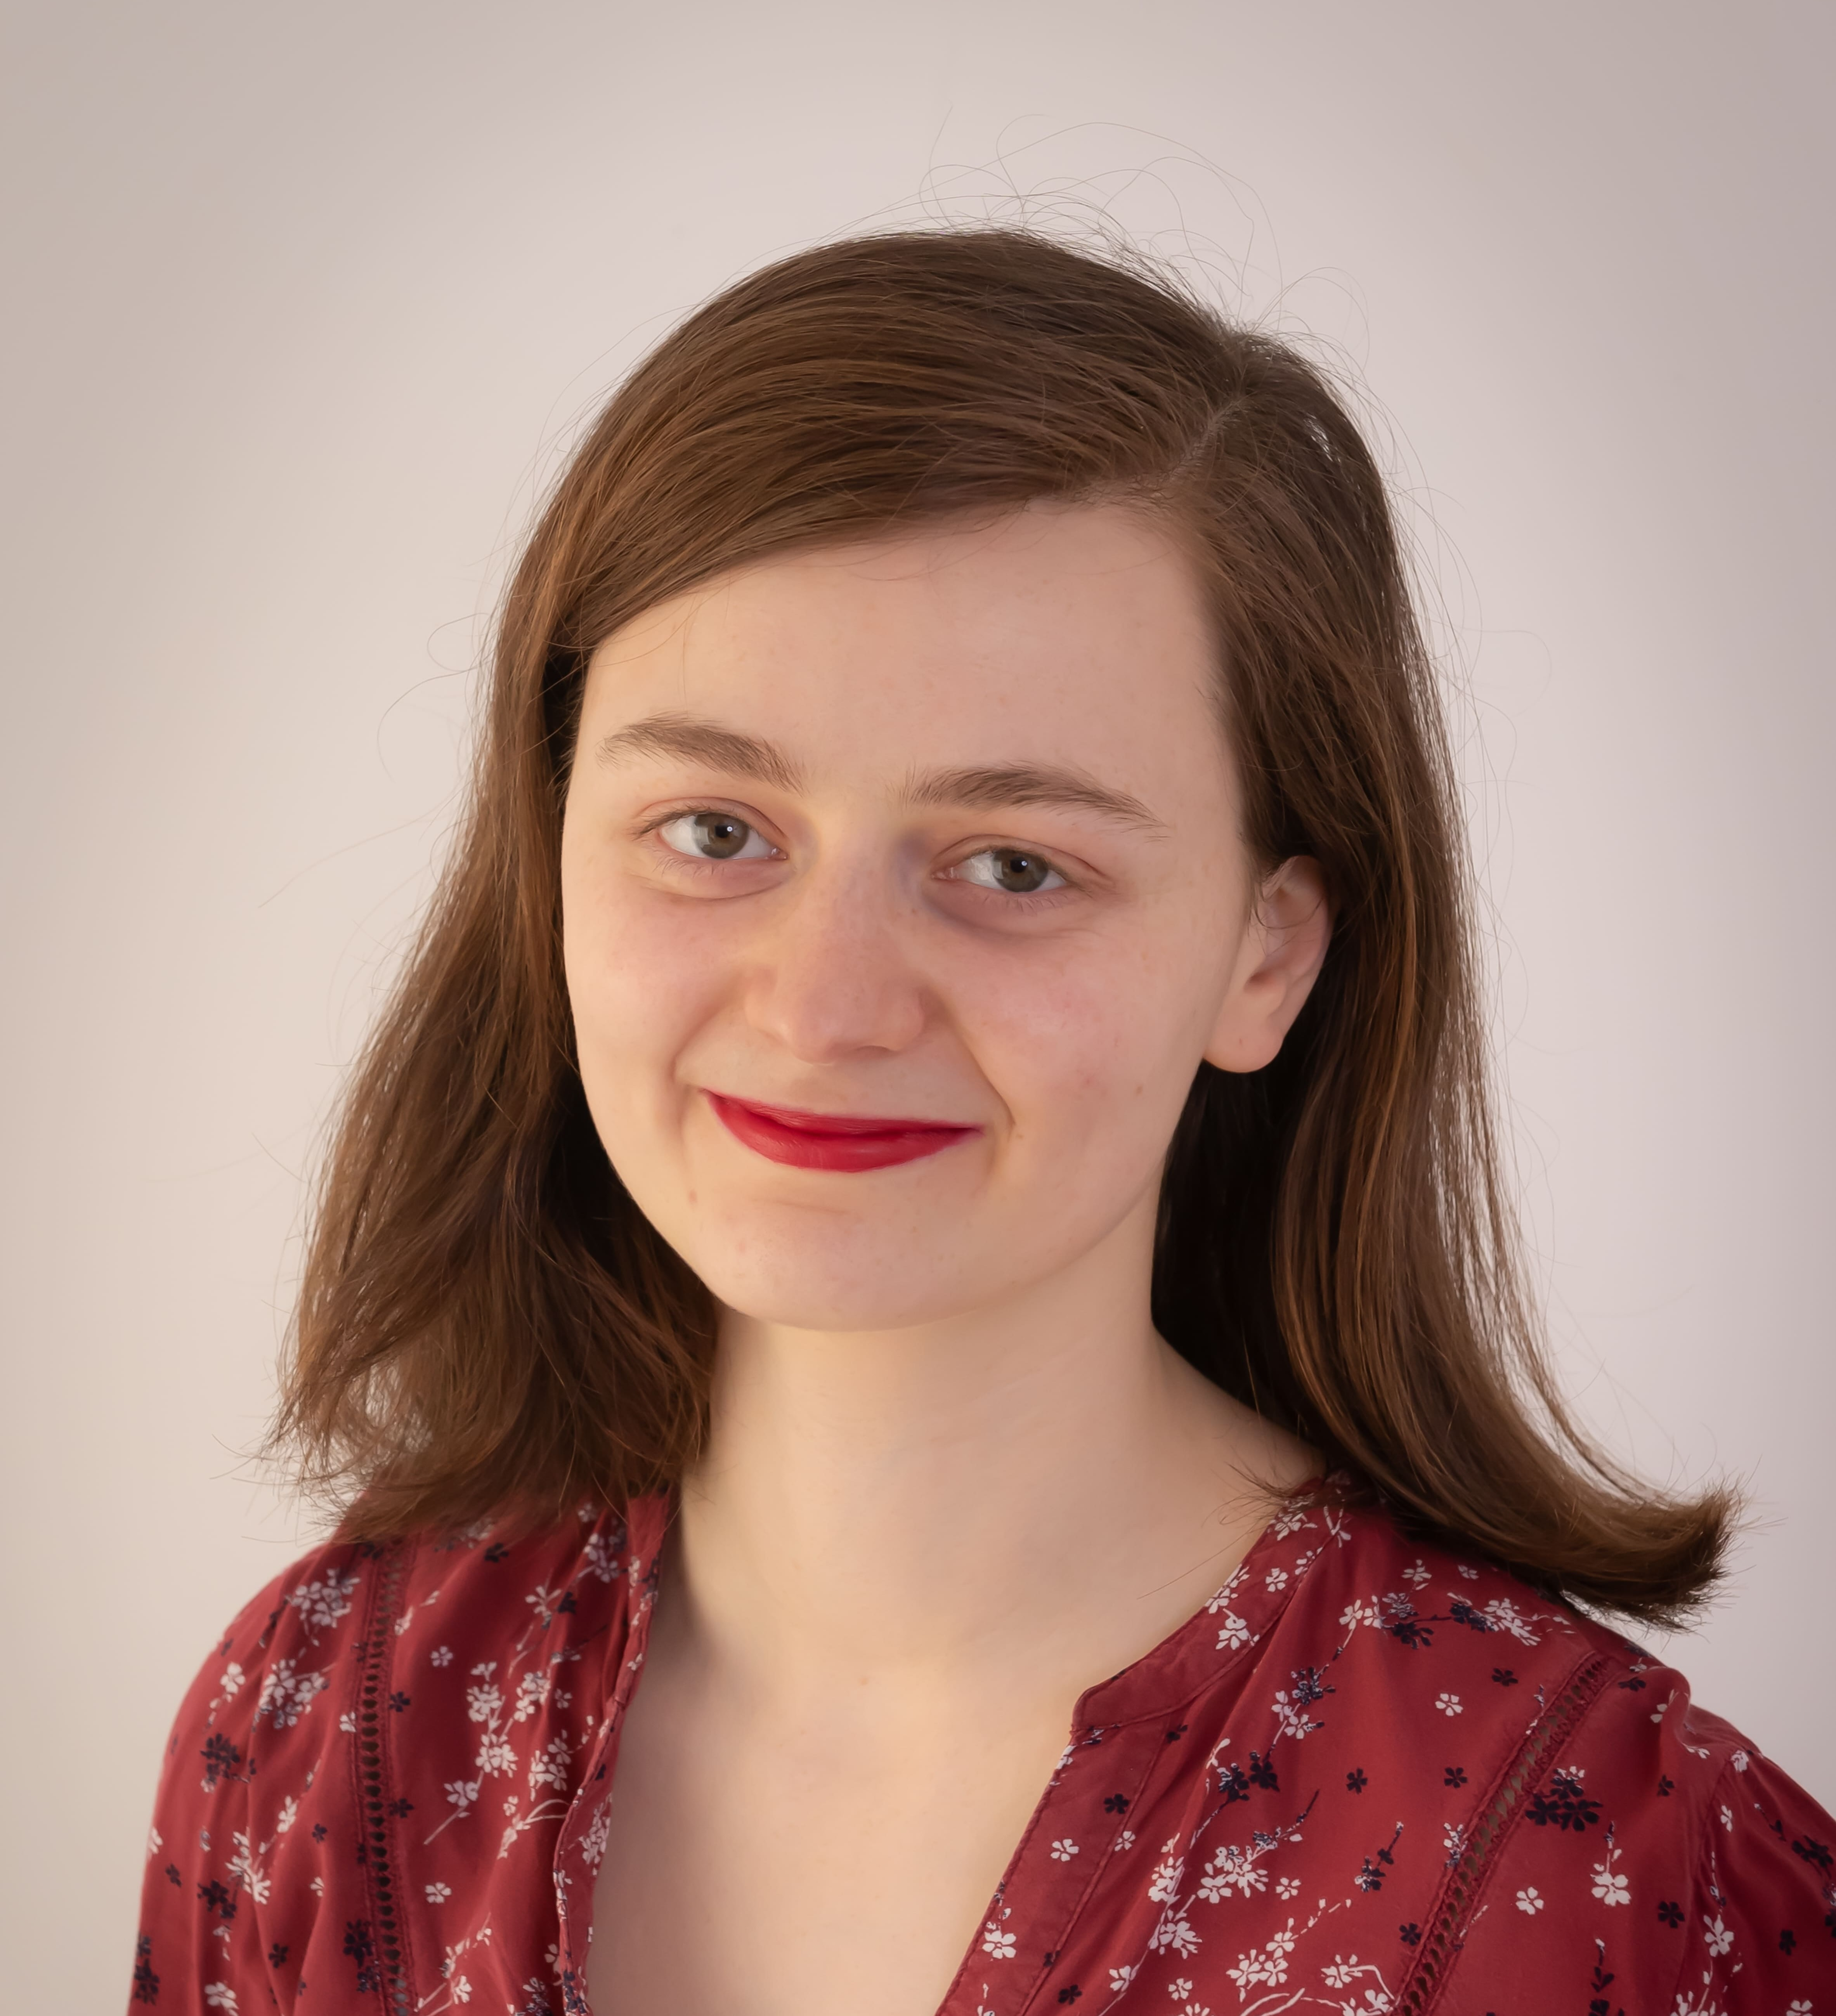
\includegraphics[width=4cm]{img/alanna.jpg}} ;
        \end{scope}

        % Position stid in the top-left corner of me
        \node[xshift=5.5cm,yshift=3.5cm,anchor=south east] at (me.south east) (stid) {
\includegraphics[width=4cm]{img/logos/logo-stid.jpg}};
        \node[anchor=south,yshift=-0.3cm] at (stid.south) (stidtexte) {DUT STID (2018-2020)};
        % \node[anchor=south,yshift=-0.4cm] at (stidtexte.south) (stage) {Stage au Cnam};

        % Position ensai below stid
        \node[anchor=south,yshift=-3.5cm] at (stid.south) (ensai) {
\includegraphics[width=4cm]{img/logos/logo-ensai.png}};
        \node[anchor=south,yshift=-0.3cm] at (ensai.south) (ensaitexte) {ENSAI (2020-2023)};
        % \node[anchor=south,yshift=-0.4cm] at (ensaitexte.south) {Filière Data Science et Data Engineering};
    \end{tikzpicture}
\end{frame}

\begin{frame}{Mon parcours professionnel}
    \begin{figure}[htb]
        \resizebox{\textwidth}{!}{
            \begin{tikzpicture}
                \begin{scope}
                    \clip (0,0)  circle (2cm) ;
                    \node[anchor=center] (me) {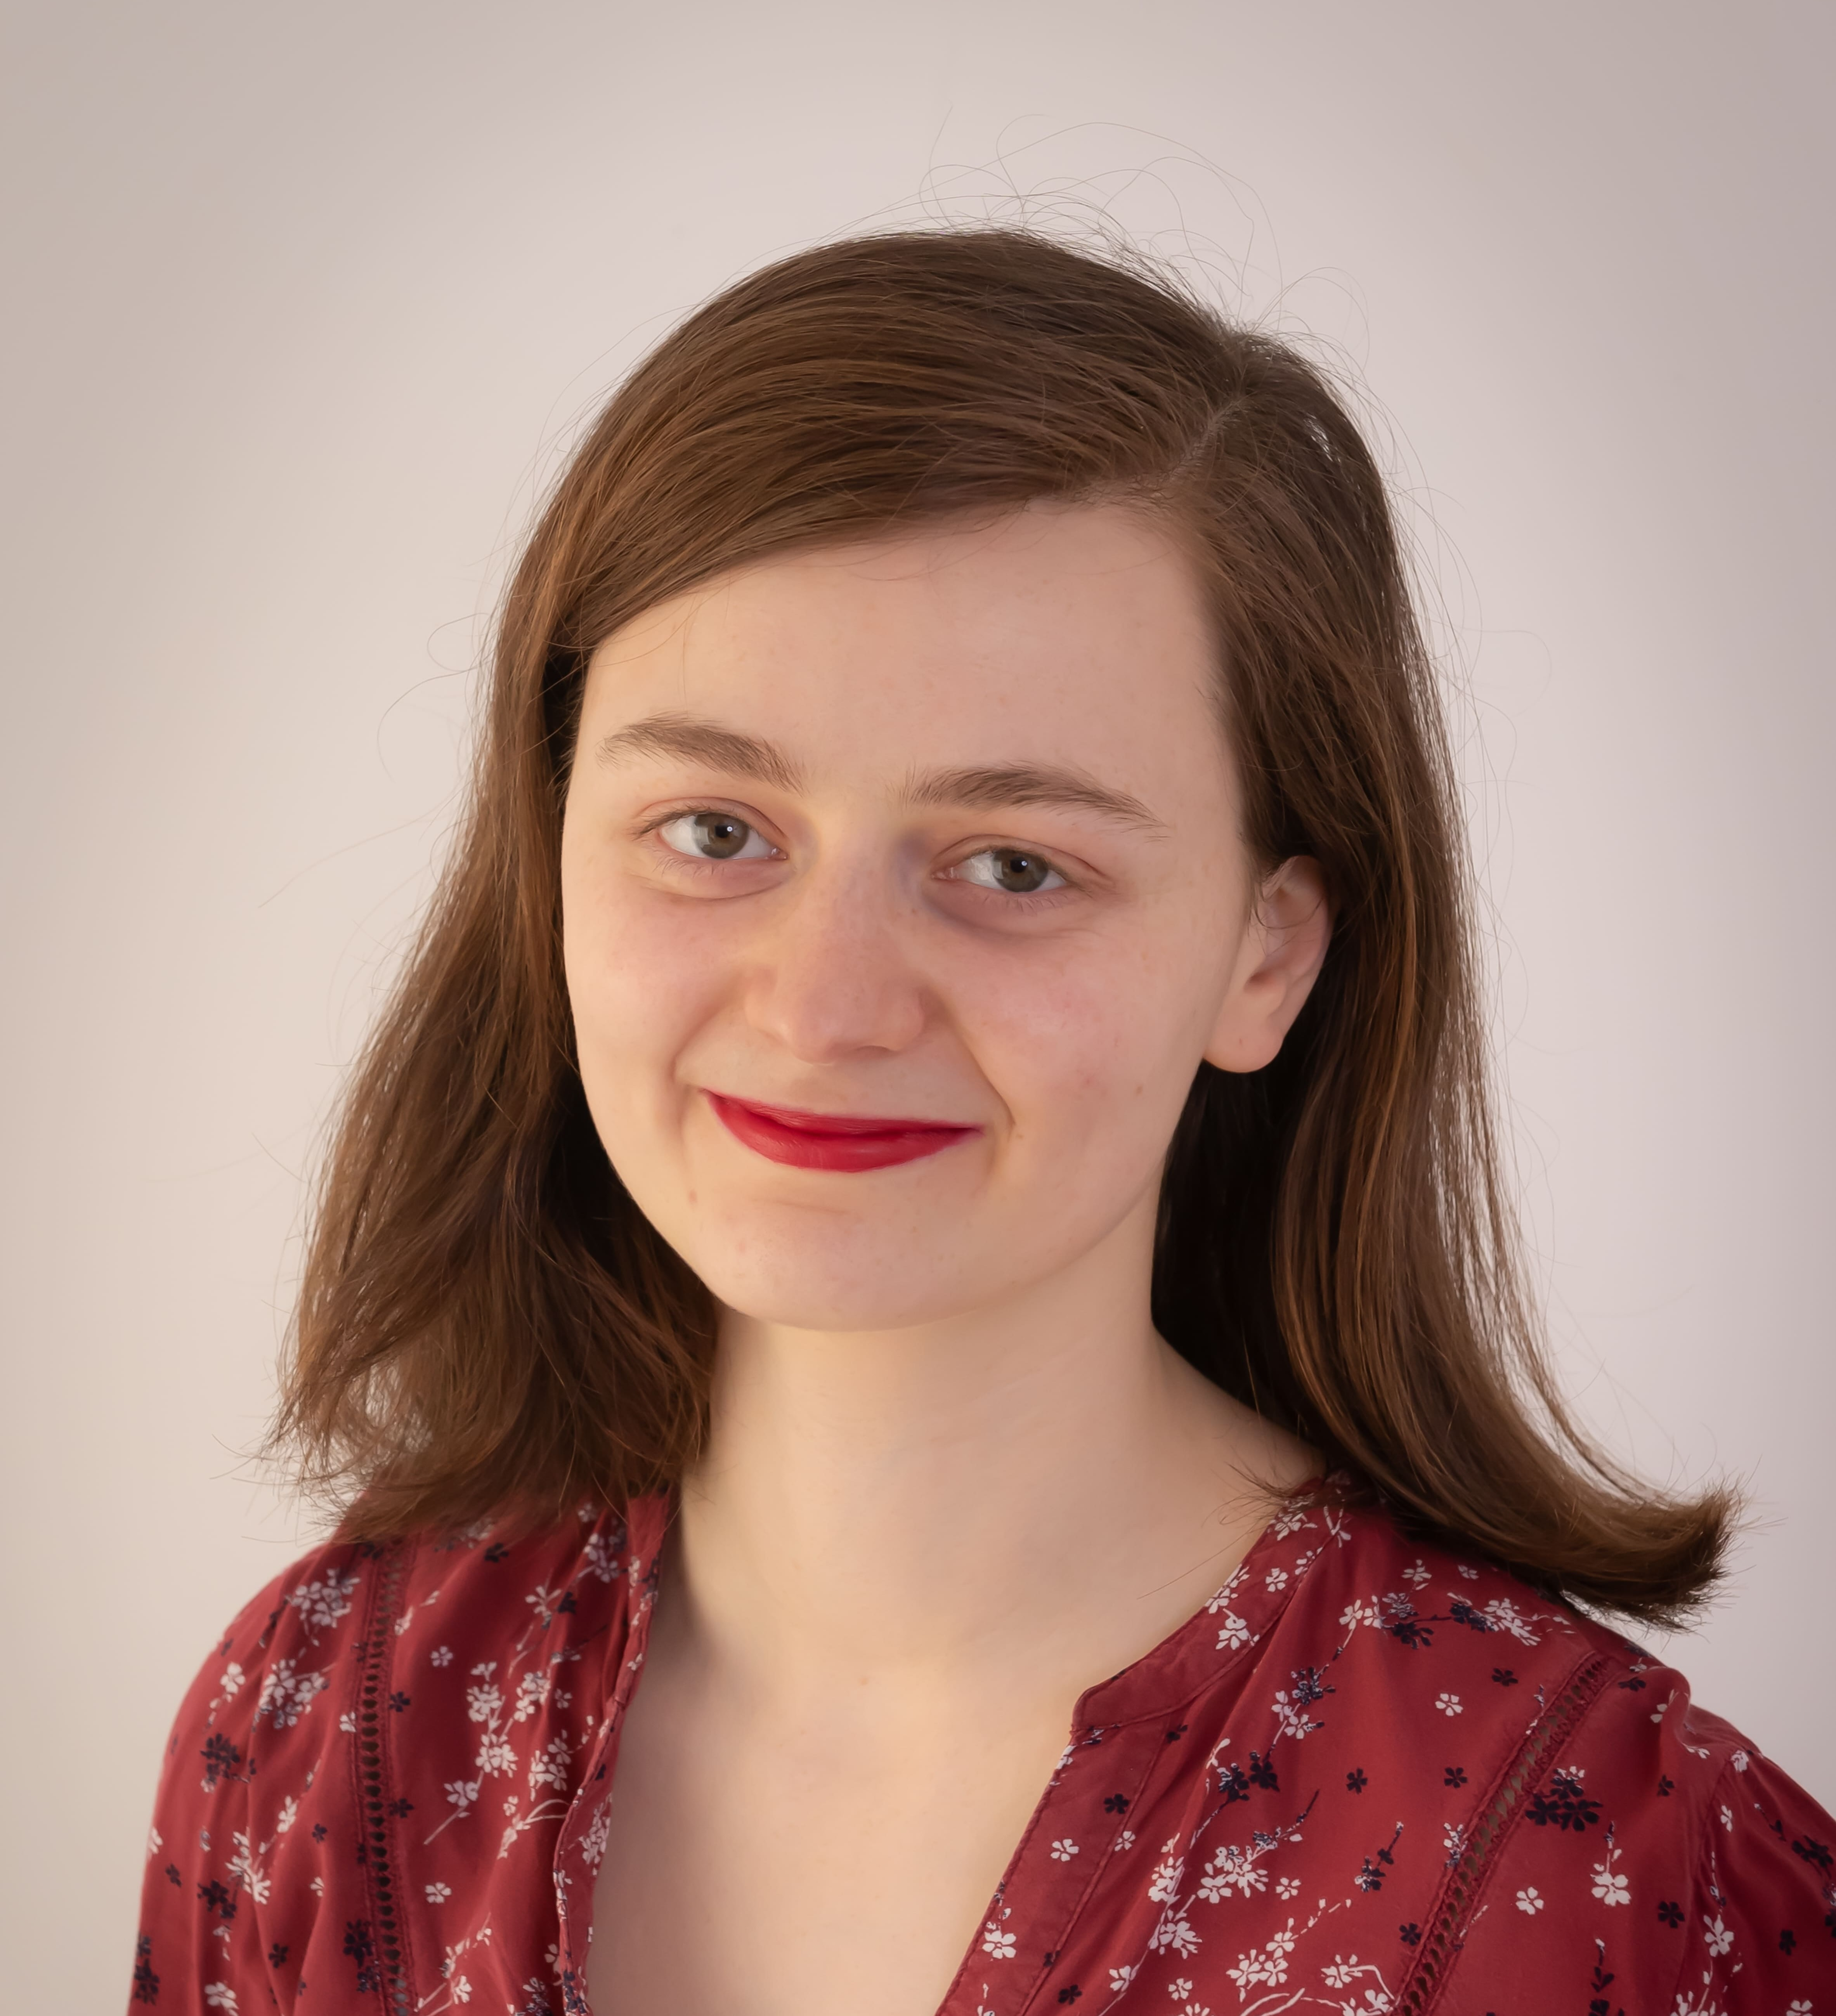
\includegraphics[width=4cm]{img/alanna.jpg}} ;
                \end{scope}

                \node [minimum width=3cm, xshift=-2cm, yshift=2.7cm] (cnam) at (me) {
\includegraphics[width=3.5cm]{img/logos/logo-cnam.png}};
                \node [minimum width=3cm, xshift=2.8cm, yshift=2.5cm] (carrefour) at (me) {
\includegraphics[width=2.2cm]{img/logos/logo-carrefour.png}};
                \node [minimum width=3cm, xshift=-4.2cm, yshift=0.8cm] (lbc) at (me) {
\includegraphics[width=4cm]{img/logos/logo-littlebigcode.png}};
                \node [minimum width=1cm, xshift=-3.8cm, yshift=-1.1cm] (graal) at (me) {
\includegraphics[width=2.5cm]{img/logos/logo-graal-systems.png}};
                \node [minimum width=3cm, xshift=4cm, yshift=0.5cm] (servier) at (me) {
\includegraphics[width=4cm]{img/logos/logo-servier}};
                \node [minimum width=3cm, xshift=-0.3cm, yshift=-2.9cm] (se) at (me) {
\includegraphics[width=3.5cm]{img/logos/logo-schneider-electric.png}};
                \node [minimum width=3cm, xshift=3.6cm, yshift=-1.7cm] (rd) at (me) {
\includegraphics[width=3cm]{img/logos/logo-renault-digital.png}};
            \end{tikzpicture}
        }
    \end{figure}
\end{frame}

\begin{frame}{Contact}
    \begin{tikzpicture}
        % Email
        \node [minimum width=3cm, xshift=0cm, yshift=0cm] (mail) {\href{mailto:alannadevlingenin@gmail.com}{
\includegraphics[width=1.5cm]{img/icon/mail.png}}};
        \node [minimum width=3cm, xshift=-1.3cm, yshift=0cm, right=of mail] (email) {~\href{mailto:alannadevlingenin@gmail.com}{alannadevlingenin@gmail.com}};

        % LinkedIn
        \node [minimum width=3cm, xshift=0cm, yshift=0.1cm, below=of mail] (linkedin) {\href{https://www.linkedin.com/in/alanna-devlin-genin/?locale=fr_FR}{
\includegraphics[width=1.5cm]{img/logos/logo-linkedin.png}}};
        \node [minimum width=3cm, xshift=-1.2cm, yshift=0cm, right=of linkedin] {~\href{https://www.linkedin.com/in/alanna-devlin-genin/?locale=fr_FR}{Alanna DEVLIN GÉNIN}};
    \end{tikzpicture}
\end{frame}

\begin{frame}{Évaluation}

    \textbf{Examen sur table} (1h30) : 40\% de la note finale

    \textbf{TP noté} (3h) : 60\% de la note finale

\end{frame}

\begin{frame}{Planning - VCOD}

    6 séances de 3h et 2 séances de 1h30\\

    \begin{itemize}
         \item Séance 1 : CM (xx septembre)
         \item Séance 2 : TP (xx/xx septembre)
         \item Séance 3 : TP (xx/xx octobre et xx/xx octobre)
         \item Séance 4 : TP (xx/xx novembre)
         \item Séance 5 : TP (xx/xx novembre)
         \item Séance 6 : Mini-projet + examen sur table (xx/xx janvier)
         \item Séance 7 : TP noté (xx/xx février)
    \end{itemize}

\end{frame}

\begin{frame}{Planning - EMS}

    6 séances de 3h et 2 séances de 1h30\\

    \begin{itemize}
         \item Séance 1 : CM (xx septembre)
         \item Séance 2 : TP (xx/xx septembre et xx/xx octobre)
         \item Séance 3 : TP (xx/xx octobre)
         \item Séance 4 : TP (xx/xx novembre)
         \item Séance 5 : TP (xx/xx novembre)
         \item Séance 6 : Mini-projet + examen sur table (xx/xx décembre)
         \item Séance 7 : TP noté (xx/xx janvier)
    \end{itemize}

\end{frame}

\begin{frame}{Avant de commencer}

    Que savez-vous des bases de données ?

    Qu'attendez-vous de ce cours ?

\end{frame}

%\begin{frame}{Programme}
%
%    \begin{itemize}
%        \item Histoire des bases de données
%        \item Caractéristiques principales des bases de données NoSQL
%        \item Typologie des bases de données NoSQL
%    \end{itemize}
%
%\end{frame}


 \begin{frame}{Sommaire}
   \setbeamertemplate{section in toc}[sections numbered]
   \tableofcontents[hideallsubsections]
 \end{frame}

\section*{Pourquoi apprendre NoSQL ? }

\subsection*{Les limites du relationnel dans le monde moderne}

\begin{frame}{Pourquoi apprendre NoSQL ? À quoi ça sert ?}
    \begin{figure}[htb]
        \centering
        \begin{tikzpicture}

            \node[inner sep=0pt, label=below:Volume] (volume) at (0,0)
                {
\includegraphics[width=.2\textwidth]{img/icon/volume.png}};

            \node[inner sep=0pt, label=below:Données non-structurées, right=of volume, xshift=2cm] (unstructured)
                {
\includegraphics[width=.2\textwidth]{img/icon/unstructured.png}};

            \node[inner sep=0pt, label=below:Scalabilité, below=of volume, yshift=-1cm] (scale)
                {
\includegraphics[width=.2\textwidth]{img/icon/scale.png}};

            \node[inner sep=0pt, label=below:Latence, right=of scale, xshift=2cm] (latency)
                {
\includegraphics[width=.2\textwidth]{img/icon/latency.png}};
        \end{tikzpicture}
    \end{figure}

    \note{
        Les bases de données relationnelles excellent pour des données structurées, stables et peu volumineuses. Mais elles montrent leurs limites dans des contextes où :

        \begin{itemize}
            \item Le volume de données explose : les tables relationnelles deviennent lentes et coûteuses à faire évoluer.
            \item Les données sont non structurées ou variées : JSON, logs, vidéos, messages, etc. ne rentrent pas dans un schéma fixe.
            \item La scalabilité horizontale est nécessaire : ajouter des serveurs pour gérer la charge est complexe avec les BDR.
            \item La latence doit être ultra-faible : les requêtes complexes (jointures) ralentissent les applications temps réel.
        \end{itemize}
    }

\end{frame}

\begin{frame}{Statistiques récentes sur l’adoption de NoSQL}

    \begin{figure}[htb]
        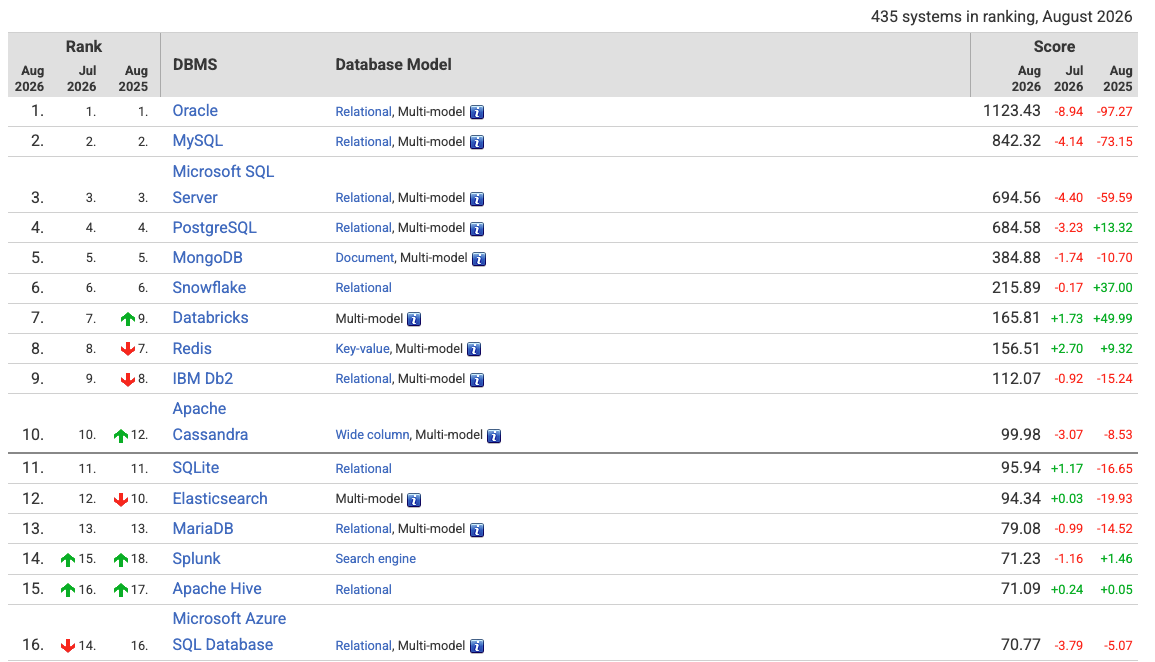
\includegraphics[width=\textwidth]{img/db-engine-ranking.png}
        \caption{Popularité des bases de données en août 2026\\\vspace{0.1cm}Source : DB Engines Ranking}
    \end{figure}

    \note{
            \begin{itemize}
            \item DB-Engines Ranking (2026) :  MongoDB, Redis et Cassandra figurent parmi les 10 bases de données les plus populaires au monde, avec une croissance annuelle de 20 à 30\% depuis 2020.
                \begin{itemize}
                    \item MongoDB : 5e position (source : \href{https://db-engines.com/en/ranking}{DB-Engines, août 2026})
                    \item Redis : 7e position
                    \item Cassandra : 10e position
                \end{itemize}
            \item Marché : le marché des bases NoSQL devrait atteindre 22 milliards de dollars d’ici 2027 (source : MarketsandMarkets).
            \end{itemize}
    }
\end{frame}

\begin{frame}{Adoption de NoSQL}
    \begin{figure}[htb]
        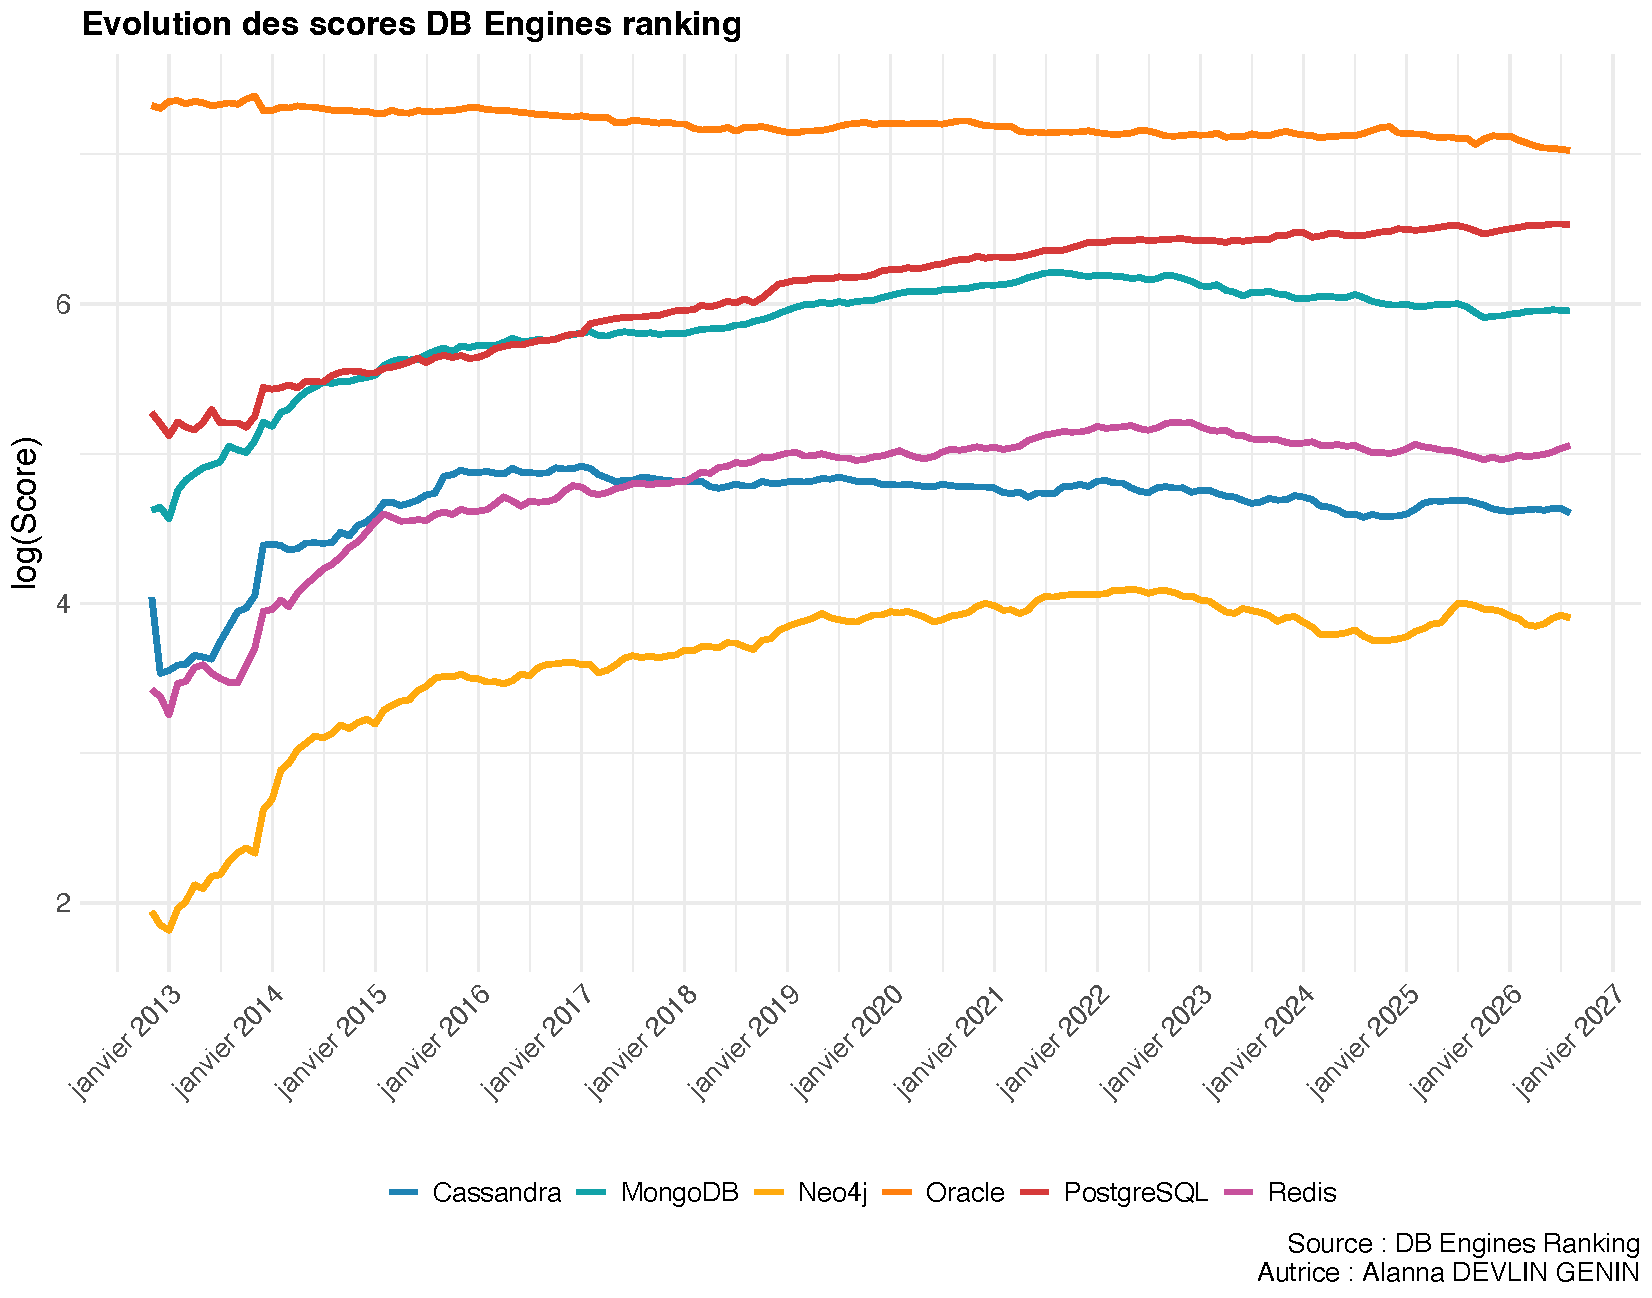
\includegraphics[width=0.85\textwidth]{img/nosql-db-engine.pdf}
    \end{figure}
\end{frame}

\begin{frame}{Popularité auprès des développeur$\cdot$euses}

    \begin{figure}[htb]
        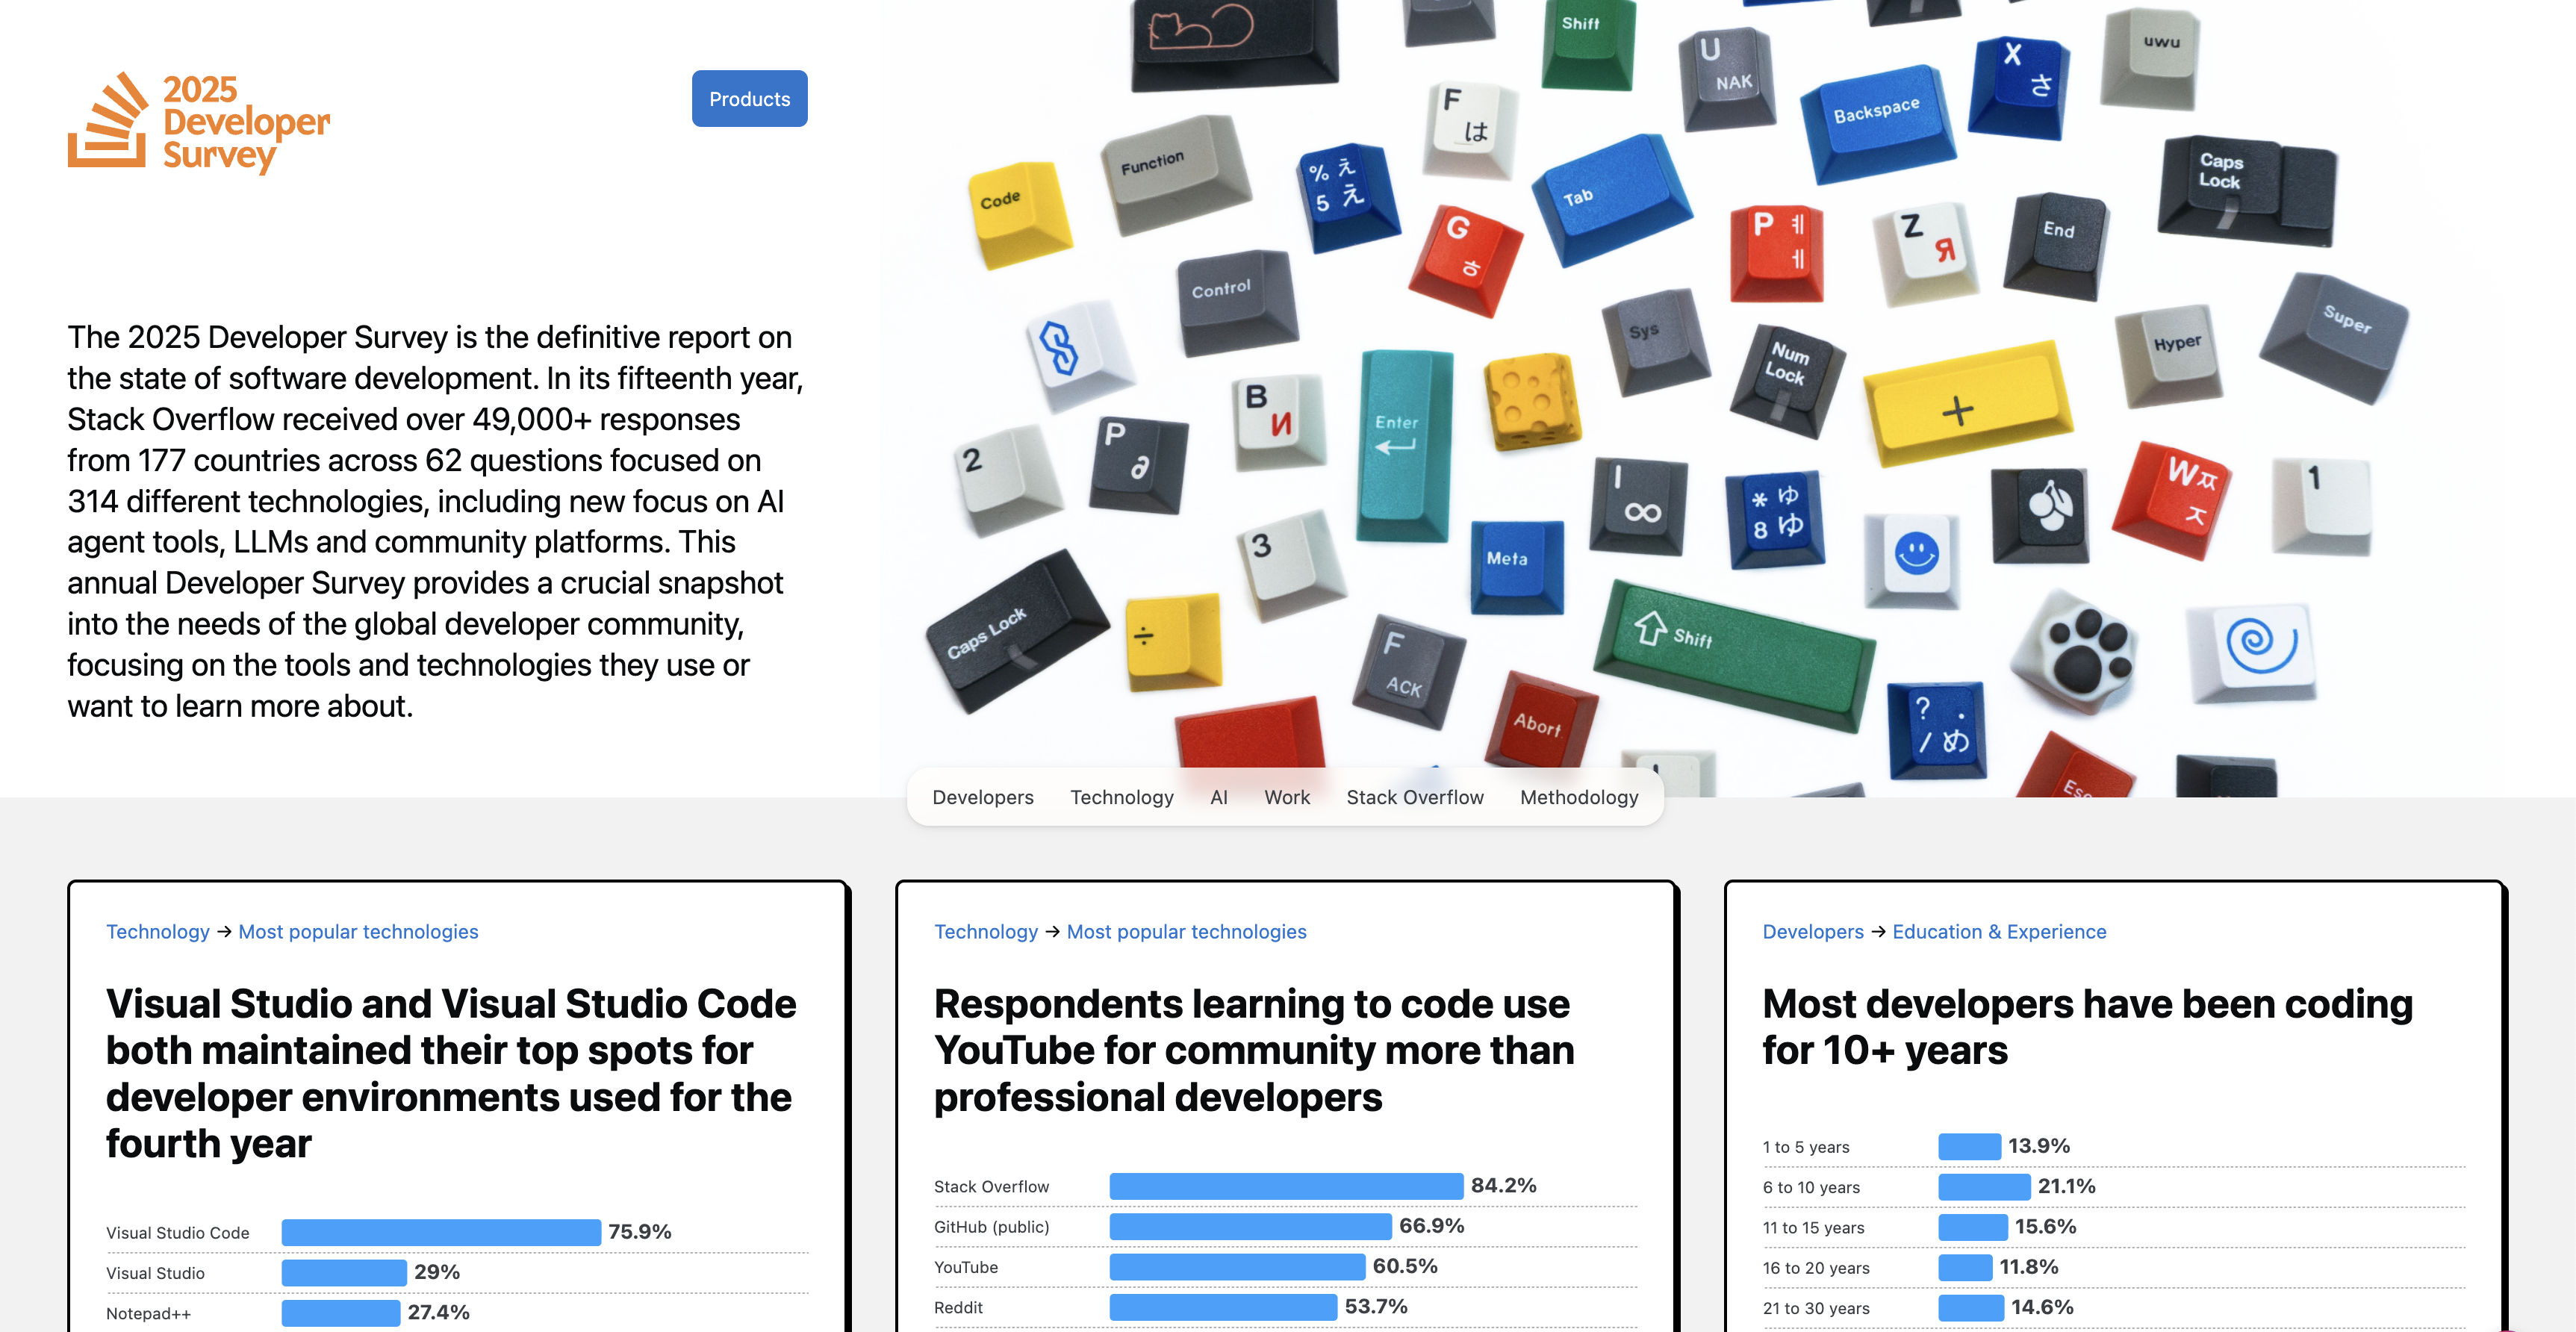
\includegraphics[width=\textwidth]{img/stack-overflow-survey-2025.png}
    \end{figure}

    \note{Enquête Stack Overflow (2025) : 60\% des développeur$\cdot$euses utilisent au moins une base NoSQL dans leurs projets, contre 45\% en 2020.}

\end{frame}

\begin{frame}{À quoi ça sert concrètement ?}

    \note{

    \begin{itemize}
        \item Flexibilité : Pas de schéma imposé → adaptation rapide aux changements de données.
        \item Performance : Lecture/écriture ultra-rapides, même avec des téraoctets de données.
        \item Scalabilité : Ajout facile de serveurs pour gérer la charge (ex : passer de 1 à 100 serveurs sans downtime).
        \item Coût : Moins cher à long terme pour les applications à forte croissance.
    \end{itemize}

    En résumé : NoSQL, c’est la réponse aux besoins modernes : données massives, variées, en temps réel, et applications qui montent en charge sans limite.
    }

\end{frame}

\begin{frame}{Cas d'utilisation de NoSQL}

    \begin{tikzpicture}
        \node[inner sep=0pt, label=below:Réseaux sociaux] (social) at (0,0)
            {
\includegraphics[width=.2\textwidth]{img/icon/social-media.png}};

        \node[inner sep=0pt, label=below:IoT, right=of social, xshift=1cm] (iot)
            {
\includegraphics[width=.2\textwidth]{img/icon/iot.png}};

        \node[inner sep=0pt, label=below:Personnalisation, right=of iot, xshift=1cm] (personnalisation)
            {
\includegraphics[width=.2\textwidth]{img/icon/customisation.png}};
    \end{tikzpicture}

     \note{
         \textbf{Réseaux sociaux} : Millions de likes/commentaires par seconde, données sociales non structurées (posts, images, vidéos).\\
         \textbf{IoT} : Des milliards de capteurs envoient des données en temps réel (température, localisation, etc.).\\
         \textbf{Personnalisation} : Analyse en temps réel des comportements utilisateurs pour recommander du contenu (Netflix, Amazon).\\
     }

\end{frame}

\begin{frame}{Cas concret : Netflix}
    % https://netflixtechblog.com/nosql-at-netflix-e937b660b4c

    \begin{figure}[htb]
        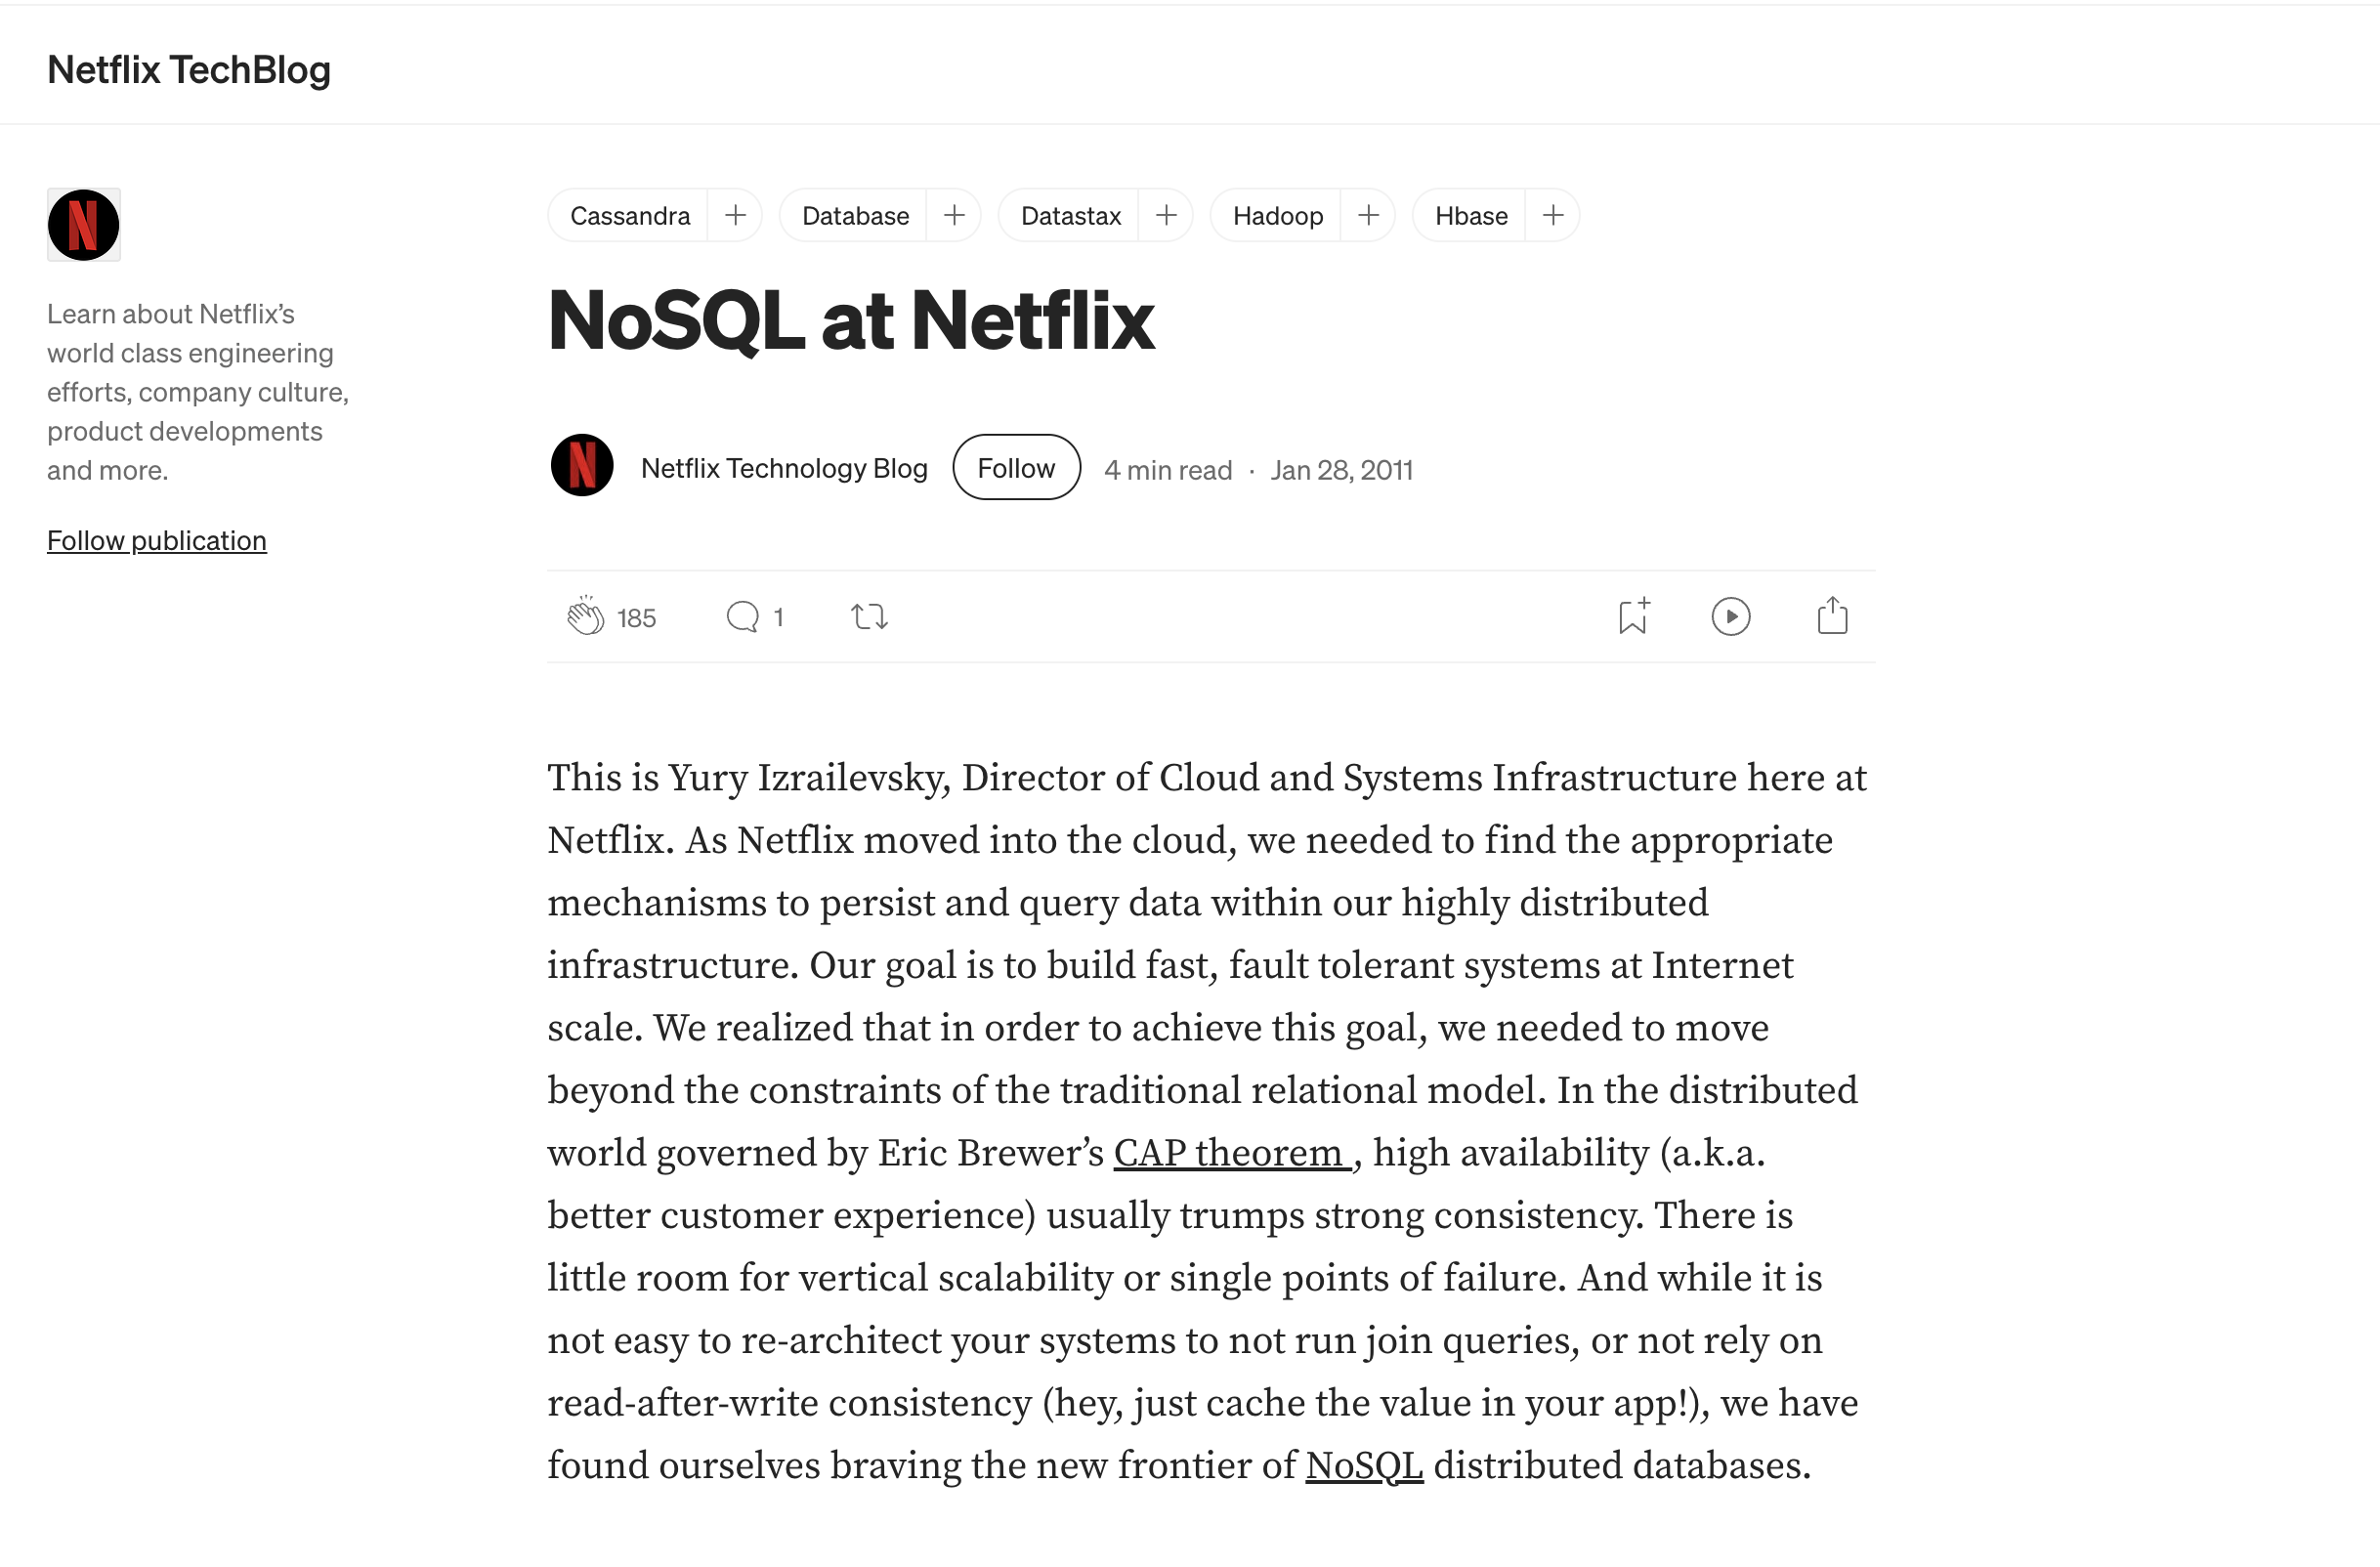
\includegraphics[width=\textwidth]{img/netflix-usecase.png}
    \end{figure}

    \note{
        Stockage des préférences utilisateurs, recommandations\\
        Cassandra, Amazon DynamoDB
    }

\end{frame}

\begin{frame}{Cas concret : Spotify}
    % https://engineering.atspotify.com/2015/1/personalization-at-spotify-using-cassandra

    \begin{figure}[htb]
        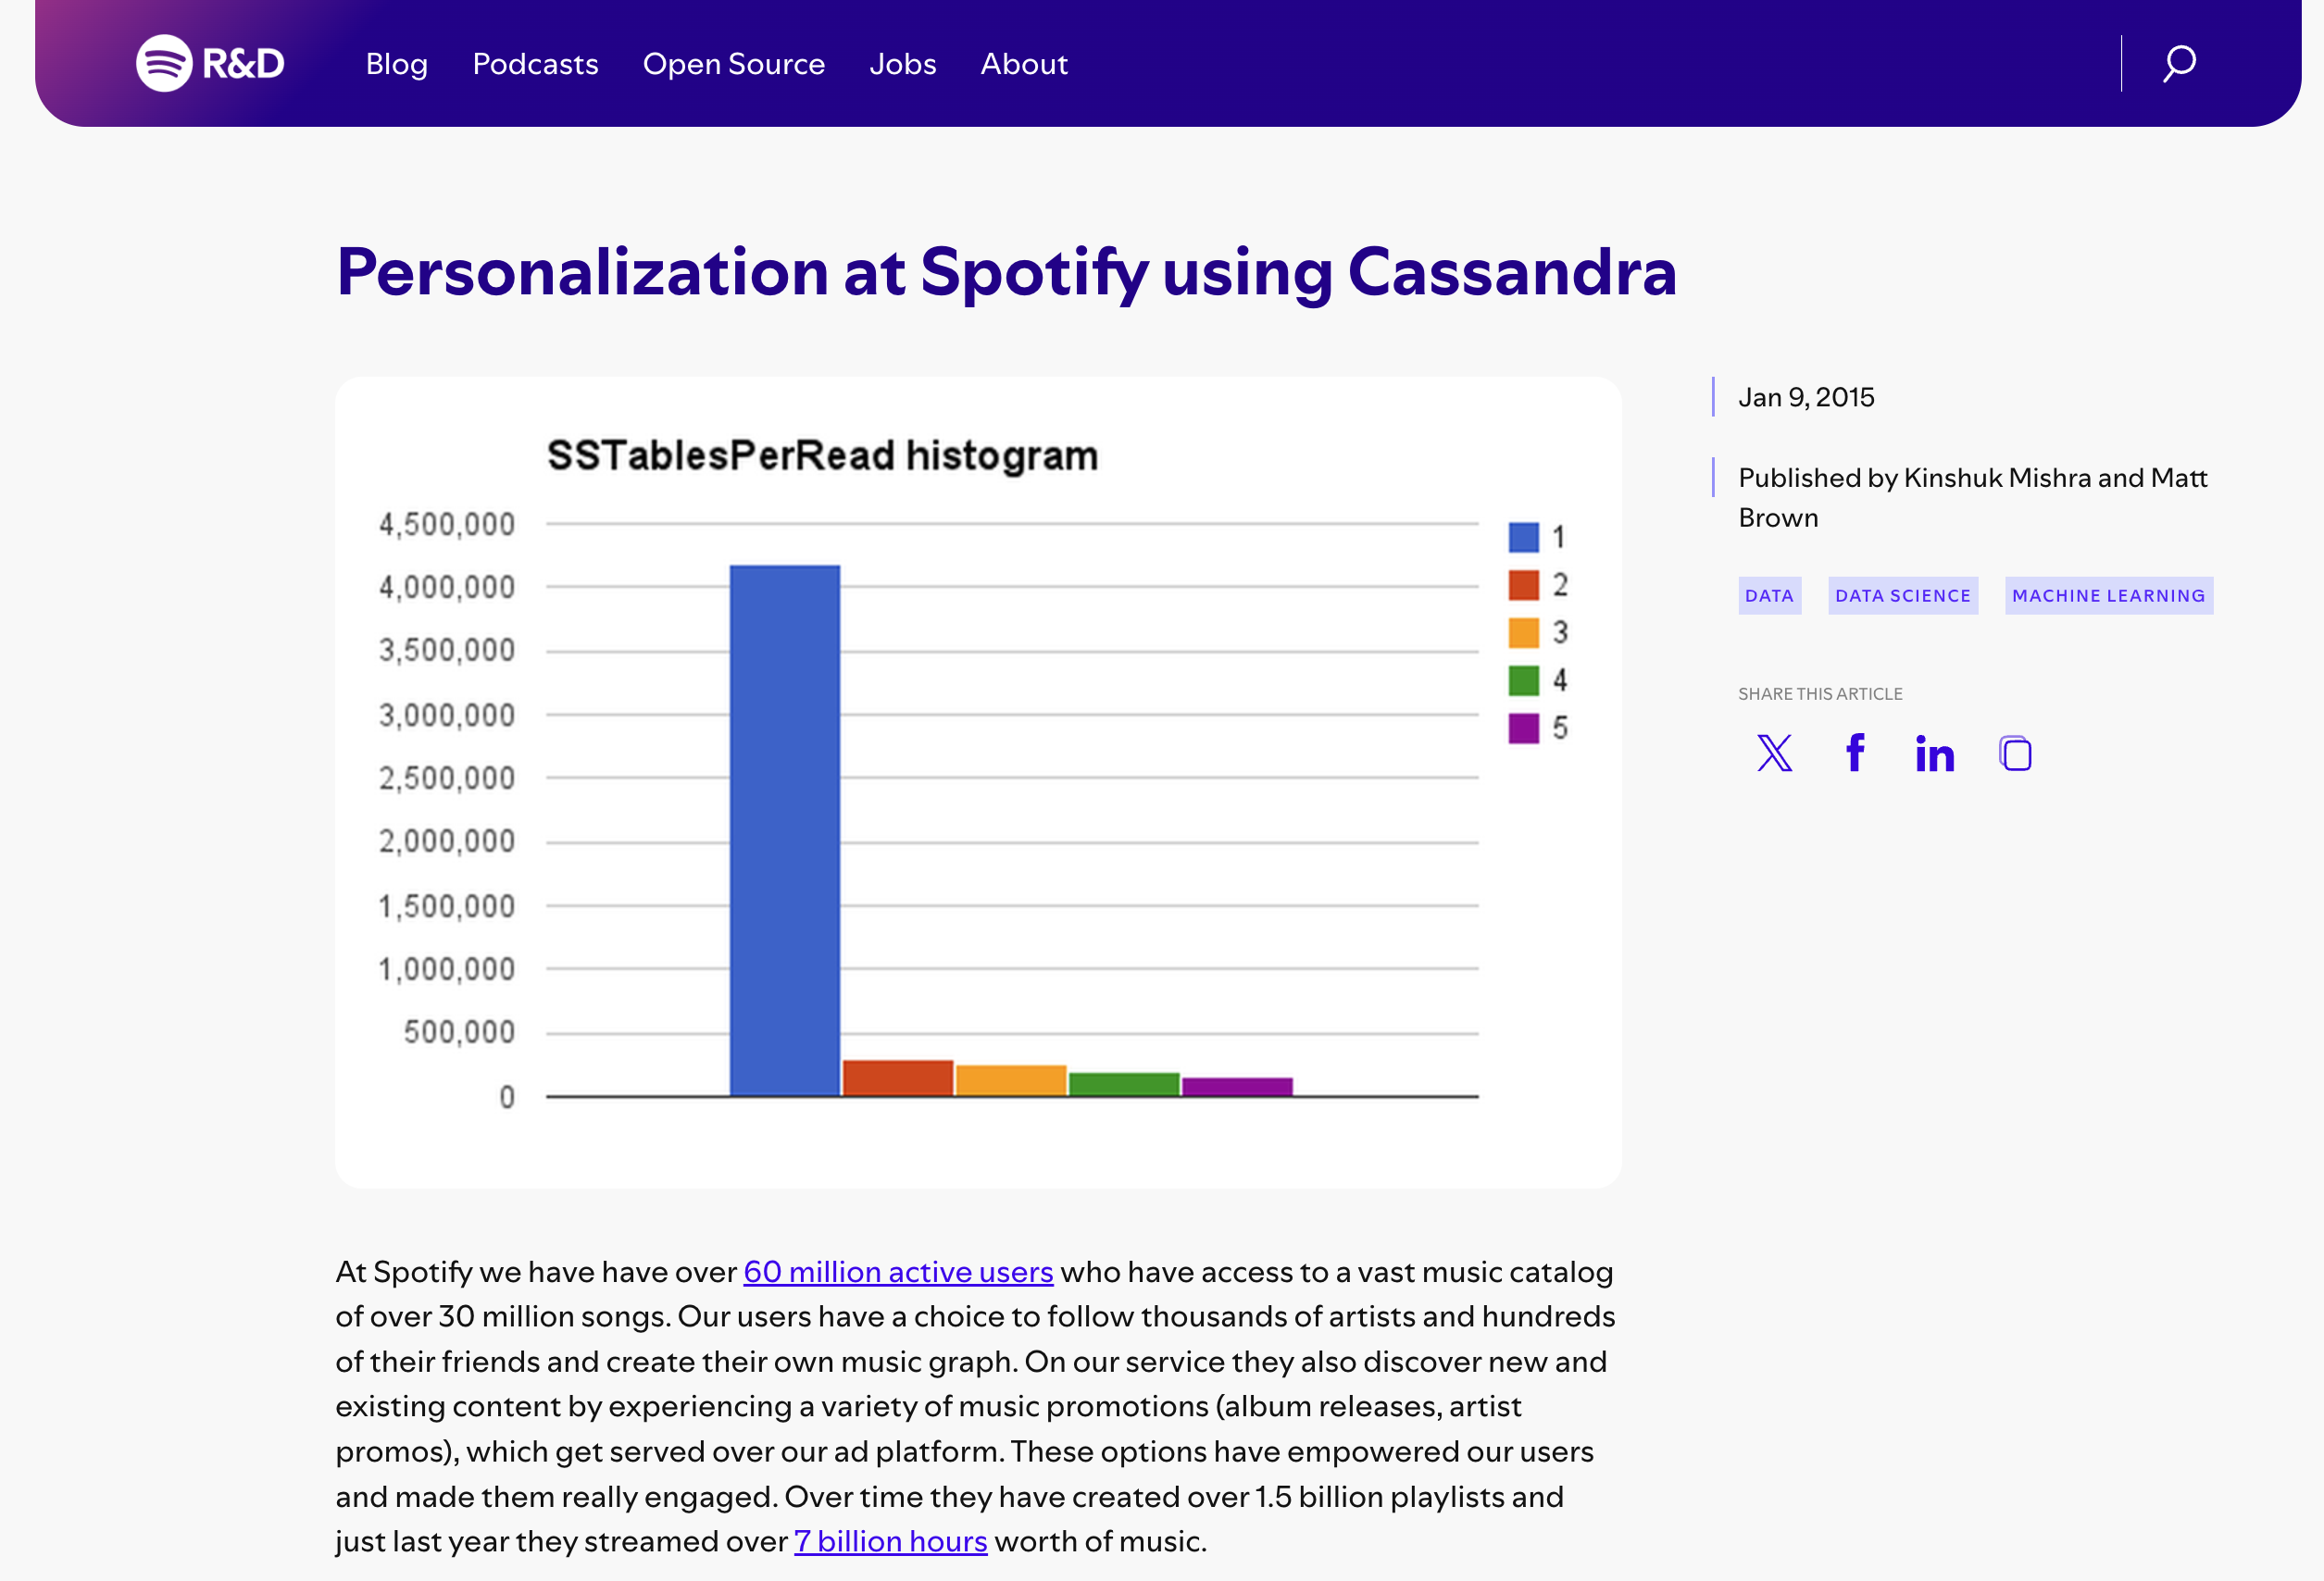
\includegraphics[width=\textwidth]{img/spotify-usecase.png}
    \end{figure}

    \note{
        Besoin : Personnaliser l'expérience utilisateur sur Spotify pour aider chaque client·e
        à découvrir du contenu pertinent selon son contexte et ses préférences, malgré
        l'abondance de choix et la diversité des comportements. \\
        Cassandra
    }

\end{frame}

\begin{frame}{Cas concret : L'Oréal}
    % https://www.mongodb.com/solutions/customer-case-studies/loreal

    \begin{figure}[htb]
        
\includegraphics[width=\textwidth]{img/loreal-usecase.png}
    \end{figure}

    \note{
        Besoin : Calculs complexes en temps réel sur d’énormes volumes de données, sans aucun temps de latence \\

        L'une des solutions internes devait permettre de se connecter à plusieurs sources de données et de rechercher des corrélations afin de conseiller le personnel sur la manière de prendre des décisions stratégiques plus efficaces. Cela implique de stocker de grands volumes de données tout en effectuant des calculs et des analyses en temps réel.\\

        Résultat : Réduction de la latence de plusieurs secondes à 10 millisecondes \\

        MongoDB
    }

\end{frame}

\section{Historique}

\begin{frame}{Retour sur les bases de données relationnelles}

    Les bases de données relationnelles permettent de stocker des \textbf{données structurées} dans des \textbf{relations} (également appelées tables).

    \begin{figure}[htb]
        \centering
        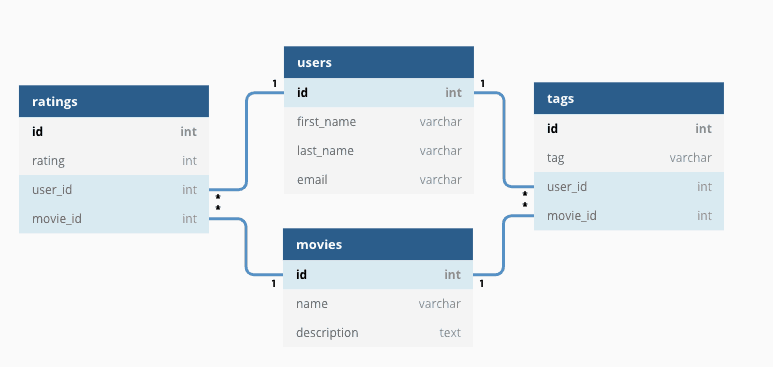
\includegraphics[width=0.8\textwidth]{img/relational-database.png}
    \end{figure}

\end{frame}

\begin{frame}{Modèle relationnel}
    \begin{tikzpicture}
    % Define classes
    \umlclass[x=0,y=0]{Customer}{
        - id : int \\
        - name : String \\
        - email : String
    }{
        + placeOrder() : void \\
        + cancelOrder() : void
    }

    \umlclass[x=5, y=0]{Order}{
        - orderId : int \\
        - date : Date
    }{
        + addProduct(Product) : void \\
        + calculateTotal() : float
    }

    \umlclass[x=5, y=-4]{Product}{
        - productId : int \\
        - name : String \\
        - price : float
    }{
        + applyDiscount(float) : void
    }

    % Relationships
    \umlassoc[arg1=1, pos1=0.2, arg2=*, pos2=0.8]{Customer}{Order}
    \umluniassoc[mult1=1, mult2=*, pos2=0.8]{Order}{Product}
    \umlcompo[mult1=1, mult2=1..*, pos2=0.8]{Customer}{Product}
\end{tikzpicture}
\end{frame}

\begin{frame}{Changement de paradigme}

    \begin{itemize}
        \item \textbf{Années 2000} : explosion du volume de données
        \item \textbf{Modèle relationnel} : limité en termes de \textbf{scalabilité} et de \textbf{flexibilité}
        \item \textbf{Nouvelles technologies} : Big Data, IoT, applications web et mobiles
    \end{itemize}

\end{frame}

\begin{frame}{Normalisation vs dénormalisation}

    \begin{itemize}
        \item \textbf{Modèle relationnel} : normalisation des données
        \item \textbf{Modèle NoSQL} : dénormalisation des données
    \end{itemize}

    Donner exemple

    Formes normales : 1NF, 2NF, 3NF, BCNF, 4NF, 5NF
\end{frame}

\begin{frame}{Formes normales}

    En informatique, une \textbf{forme normale} est un ensemble de règles visant à organiser les données dans une base de données relationnelle afin de minimiser la redondance et d'améliorer l'intégrité des données.
    % https://www.datacamp.com/tutorial/normalization-in-sql
    \begin{itemize}
        \item \textbf{1NF} : élimination des groupes de répétition
        \item \textbf{2NF} : élimination des dépendances partielles
        \item \textbf{3NF} : élimination des dépendances transitives
        \item \textbf{BCNF} : Boyce-Codd Normal Form
        \item \textbf{4NF} : élimination des dépendances multivaluées
        \item \textbf{5NF} : élimination des dépendances de jointure
%        \item \textbf{DNF} : forme dénormalisée
%        \item \textbf{ENF} : forme normalisée étendue
%        \item \textbf{ONF} : forme normale optimale
%        \item \textbf{TNF} : forme normale temporelle
%        \item \textbf{INF} : forme normale d'inclusion
%        \item \textbf{PNF} : forme normale de projection
%        \item \textbf{KNF} : forme normale de clé
%        \item \textbf{LNF} : forme normale logique
%        \item \textbf{MNF} : forme normale minimale
%        \item \textbf{NNF} : forme normale négative
    \end{itemize}

\end{frame}

\begin{frame}{Application de formes normales}

    Exemple de formes normales sur une table de base de données relationnelle.

\end{frame}

\begin{frame}{OLAP vs OLTP}

    \begin{itemize}
        \item \textbf{OLTP} : Online Transaction Processing
        \item \textbf{OLAP} : Online Analytical Processing
    \end{itemize}

    OLAP : requêtes complexes, agrégations, analyses multidimensionnelles

    OLTP : transactions, insertions, mises à jour, suppressions

\end{frame}


\section{Introduction au NoSQL}

\begin{frame}{Pourquoi NoSQL ?}

    \begin{itemize}
        \item Stockage et de traitement d'une grande quantité de données
        \item Scalabilité
        \item Haute disponibilité
        \item Réplication
        \item Partitionnement
        \item Indexation
    \end{itemize}

\end{frame}

\begin{frame}{Mais que signifie NoSQL ?}

    \begin{definitionbox}
        NoSQL signifie Not Only SQL ou No SQL.
    \end{definitionbox}

    \pause

        En 2009, Johan Oskarsson définit NoSQL comme un terme générique pour désigner les bases de données qui ne sont pas des bases de données relationnelles.

\end{frame}

\section{Concepts fondamentaux}

\begin{frame}{Caractéristiques principales du NoSQL}

    \begin{itemize}
        \item Schéma flexible
        \item Scalabilité
        \item Haute disponibilité
        \item Réplication
        \item Partitionnement
        \item Indexation
        \item Transactions
    \end{itemize}
\end{frame}

\subsection{Scalabilité}

\begin{frame}{Scalabilité}

    \begin{figure}[htb]
        \centering
        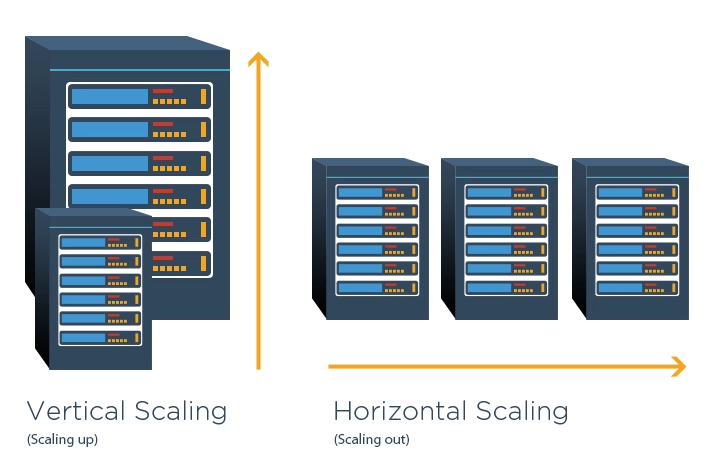
\includegraphics[width=0.9\textwidth]{img/horizontal-vs-vertical-scaling.png}
    \end{figure}

\end{frame}

\begin{frame}{Qu'est-ce que la scalabilité ?}

    Scalabilité horizontale : Ajout de machines pour augmenter la capacité de stockage et de traitement

    Scalabilité verticale : Ajout de ressources (CPU, RAM, Disque) sur une machine existante

    NoSQL databases are designed to scale out horizontally, meaning you can add more servers or nodes to the database cluster to handle increased data volume, traffic, or performance requirements. On the other hand, SQL databases often scale up vertically by adding more CPU, RAM, or storage capacity to a single server to handle increased demands.
\end{frame}

% ----------------------------------------------------------------------------------------------------------------------
% ----------------------------------------------------------------------------------------------------------------------
% ----------------------------------------------------------------------------------------------------------------------

\subsection{Partitionnement}

\begin{frame}{Qu'est-ce que le partitionnement ?}

    \begin{definitionbox}
        Le \textbf{partitionnement} (ou \textit{partitioning} en anglais) consiste à séparer les données en plusieurs \textit{chunks}.
    \end{definitionbox}

    \begin{figure}[htb]
        \begin{tikzpicture}
            \node[anchor=south west,scale=0.6,label=below:Data source] (singlefile) {\singlefile};

            \node[anchor=south west,scale=0.6,right=of singlefile,xshift=2cm,yshift=-0.5cm] (filechunck) {\filechunck};

            \draw [->, thick, draw=gray] ([yshift=-0.3cm]singlefile.east) -- node [above] {Chunking} (filechunck.west);
        \end{tikzpicture}
    \end{figure}

\end{frame}

\begin{frame}[standout]

    Partitionnement ou sharding ?

\end{frame}

\begin{frame}{Partitionnement vs sharding}

    \begin{definitionbox}
        Le \textbf{partitionnement} est une technique de division des données en plusieurs parties.
    \end{definitionbox}
    \pause
    \begin{definitionbox}
        Le \textbf{sharding} est une technique de distribution des données sur plusieurs n\oe{}uds.
    \end{definitionbox}

\end{frame}

\begin{frame}{Partitionnement vs sharding}
    \begin{figure}[htb]
        \resizebox{\textwidth}{!}{
        \begin{tikzpicture}
            \Large
            % Colors and styles
            \definecolor{lightblue}{RGB}{91,155,213}
            \definecolor{lightpurple}{RGB}{173,124,228}
            \definecolor{lightgray}{RGB}{239,240,241}

            \tikzstyle{db} = [shape border rotate=90, draw, thick, aspect=2, minimum height=8cm, minimum width=6cm, cylinder body fill=lightblue, cylinder end fill=lightgray]
            \tikzstyle{table cell} = [font=\scriptsize, draw=none]

            % Partitioning DB
            \node[db, cylinder, fill=lightgray, text centered] (partitioning) at (0,0) {};
            \node[above=of partitioning] {\textbf{PARTITIONING}};

            % Sharding DB
            \node[db, cylinder, text centered, label=below:\textbf{\Large Shard 1}, fill=lightpurple, right=of partitioning,xshift=3cm] (shard1) {};
            \node[db, cylinder, text centered, label=below:\textbf{\Large Shard 2}, fill=lightpurple, right=of shard1] (shard2) {};
            \node[above=of shard1,xshift=3.5cm] {\textbf{SHARDING}};

            \node[right=of partitioning,xshift=-0.1cm] {\textbf{VERSUS}};

            % Partitioning table
            \node[anchor=center,yshift=1.5cm] at (partitioning) (part1) {
                \begin{tabular}{|c|c|}
                    \hline
                    ID & Name \\ \hline
                    1 & Alice \\ \hline
                    2 & Bob \\ \hline
                    3 & Camille \\ \hline
                \end{tabular}
            };

            \node[anchor=center,below=of part1,yshift=1cm] (part2) {
                \begin{tabular}{|c|c|}
                    \hline
                    ID & Name \\ \hline
                    4 & Diane \\ \hline
                    5 & Elodie \\ \hline
                    6 & Fabrice \\ \hline
                \end{tabular}
            };

            % Sharding tables
            \node[anchor=center] at (shard1) {
                \begin{tabular}{|c|c|}
                    \hline
                    ID & Name\\ \hline
                    1 & Alice \\ \hline
                    2 & Bob \\ \hline
                    3 & Camille \\ \hline
                \end{tabular}
            };

            \node[anchor=center] at (shard2) {
                \begin{tabular}{|c|c|}
                    \hline
                    ID & Name\\ \hline
                    4 & Diane \\ \hline
                    5 & Elodie \\ \hline
                    6 & Fabrice \\ \hline
                \end{tabular}
            };

        \end{tikzpicture}
        }
    \end{figure}

\end{frame}

\begin{frame}{Différentes stratégies de partitionnement}
    \begin{columns}[onlytextwidth] % align columns
        \begin{column}{.48\textwidth}
            \begin{figure}[htb]
                \resizebox{\textwidth}{!}{
                \begin{tikzpicture}
                    % Include the file stack icon
                    \node[anchor=south west,scale=0.6,label=below:Data source] at (0,-1) (filechunck) {\filechunck};

                    \node[
                        database,ultra thick,database radius=1cm,
                        database segment height=0.5cm,
                        database top segment={draw=black,fill=customred},
                        database middle segment={draw=black,fill=customred},
                        database bottom segment={draw=black,fill=customred},
                        scale=0.6
                    ] at (5,2) (shard1) {};

                    \node[
                        database,ultra thick,database radius=1cm,
                        database segment height=0.5cm,
                        database top segment={draw=black,fill=customblue},
                        database middle segment={draw=black,fill=customblue},
                        database bottom segment={draw=black,fill=customblue},
                        scale=0.6
                    ] at (5,0) (shard2) {};

                    \node[
                        database,ultra thick,database radius=1cm,
                        database segment height=0.5cm,
                        database top segment={draw=black,fill=customgreen},
                        database middle segment={draw=black,fill=customgreen},
                        database bottom segment={draw=black,fill=customgreen},
                        scale=0.6
                    ] at (5,-2) (shard3) {};

                    % links
                    \draw [->, thick, draw=gray] (filechunck.east) -- node [above] {\textcolor{gray}{\bf ?}} (shard1.west);
                    \draw [->, thick, draw=gray] (filechunck.east) -- node [above] {\textcolor{gray}{\bf ?}} (shard2.west);
                    \draw [->, thick, draw=gray] (filechunck.east) -- node [above] {\textcolor{gray}{\bf ?}} (shard3.west);
                \end{tikzpicture}
                }
            \end{figure}
        \end{column}%
        \hfill%
        \begin{column}{.48\textwidth}
            \small
            \begin{itemize}
                \item Partitionnement par tourniquet
                \item Partitionnement par intervalle
                \item Partitionnement par clé/liste
                \item Partitionnement par hachage
            \end{itemize}
        \end{column}%
    \end{columns}
\end{frame}

\begin{frame}{Cas d'usage}

    Camille Lemoine est propriétaire d'une chaîne de trois restaurants situés à Paris, Londres et Dublin. Elle souhaite stocker les données de ses clients dans une base de données en fonction de ses différents restaurants.

    \begin{table}[]
        \begin{tabular}{|c|c|c|c|c|}
        \hline
        \rowcolor{lipstick}\color{white}\textbf{Identifiant} & \color{white}\textbf{Prénom} & \color{white}\textbf{Nom}  & \color{white}\textbf{Âge} & \color{white}\textbf{Ville}  \\\hline
        1000                 & Alice           & Dupont        & 30           & Paris \\
        1001                 & Bob             & Brown         & 39           & Londres \\
        1002                 & Charlie         & O'Brien       & 26           & Dublin \\
        1003                 & Daniel          & Doyle         & 42           & Dublin \\
        1004                 & Edna            & McCarthy      & 58           & Dublin \\
        1005                 & Fabienne        & Lenoir        & 66           & Paris \\
        1006                 & Gilles          & Morvan        & 71           & Paris \\
        \hline
        \end{tabular}
    \end{table}

    Elle vous demande de l'aider à choisir la meilleure stratégie de partitionnement pour stocker les données de ses clients en fonction de leur localisation.

\end{frame}

% ------------------------------------------------------------------------------------------------------------------------------------------------------------------------
%                                                                   Partitionnement par tourniquet
% ------------------------------------------------------------------------------------------------------------------------------------------------------------------------

\begin{frame}{Partitionnement par tourniquet}

    \begin{definitionbox}
        Le \textbf{partitionnement par tourniquet} (\textit{round-robin partitioning} en anglais) est une méthode de distribution des données où chaque enregistrement est successivement assigné à l'une des partitions disponibles de \textbf{manière cyclique}, assurant une répartition équilibrée de la charge
    \end{definitionbox}

    \pause

    \examplebox{
        \textbf{Comment assigner une donnée $i$ à un n\oe{}ud $n_j$ ?}

        La donnée située à l'index $i$ sera assignée au n\oe{}ud d'index $j$ noté $n_j$ avec \textit{$n_j$ = i mod n} et $n$ est le nombre de n\oe{}uds.
    }

\end{frame}


\begin{frame}{Partitionnement par tourniquet}
    \begin{figure}[htb]
        \resizebox{\textwidth}{!}{
        \begin{tikzpicture}

            \node[] at (-1.5,0) (users) {
                \begin{tabular}{|c|c|c|}
                    \hline
                    \textbf{ID} & \textbf{Prénom} & \textbf{Nom} \\ \hline
                    \only<2->{\rowcolor{customred!20}}1000 & Alice & Dupont \\
                    \only<3->{\rowcolor{customblue!20}}1001 & Bob & Brown \\
                    \only<4->{\rowcolor{customgreen!20}}1002 & Charlie & O'Brien \\
                    \only<5->{\rowcolor{customred!20}}1003 & Daniel & Doyle \\
                    \only<6->{\rowcolor{customblue!20}}1004 & Edna & McCarthy \\
                    \only<7->{\rowcolor{customgreen!20}}1005 & Fabienne & Lenoir \\
                    \only<8>{\rowcolor{customred!20}}1006 & Gilles & Morvan \\\hline
                \end{tabular}
                };

            \node[above=of users,text width=10cm,align=center] (question) {Comment partitionner par tourniquet\\ selon l'ID de l'utilisateur ?};
            \node[below=of users,text width=10cm,align=center] (remarque) {On considérera qu'un modulo 0 \\(ie 3 mod 3 = 0) correspond au n\oe{}ud 3.};

            \onslide<2>{\node[below=of users,yshift=-1.5cm] (alice) {Alice : user ID mod n = 1000 mod 3 = 1};}

            \node[
                database,ultra thick,database radius=1cm,
                database segment height=0.5cm,
                database top segment={draw=black,fill=customred},
                database middle segment={draw=black,fill=customred},
                database bottom segment={draw=black,fill=customred},
                scale=0.8,
                label=below:N\oe{}ud 1
            ] at (5,3) (shard1) {};

            \node[
                database,ultra thick,database radius=1cm,
                database segment height=0.5cm,
                database top segment={draw=black,fill=customblue},
                database middle segment={draw=black,fill=customblue},
                database bottom segment={draw=black,fill=customblue},
                scale=0.8,
                label=below:N\oe{}ud 2
            ] at (5,0) (shard2) {};

            \node[
                database,ultra thick,database radius=1cm,
                database segment height=0.5cm,
                database top segment={draw=black,fill=customgreen},
                database middle segment={draw=black,fill=customgreen},
                database bottom segment={draw=black,fill=customgreen},
                scale=0.8,
                label=below:N\oe{}ud 3
            ] at (5,-3) (shard3) {};

            \onslide<2-4>{\node[right=of shard1, xshift=0.1cm] (users1) {
                \begin{tabular}{|c|c|c|}
                    \hline
                    \textbf{ID} & \textbf{Prénom} & \textbf{Nom} \\
                    1000 & Alice & Dupont \\
                    \hline
                \end{tabular}
            };}

            \onslide<5-7>{\node[right=of shard1, xshift=0.1cm] (users1) {
                \begin{tabular}{|c|c|c|}
                    \hline
                    \textbf{ID} & \textbf{Prénom} & \textbf{Nom} \\
                    1000 & Alice & Dupont \\
                    1003 & Daniel  & Doyle \\
                    \hline
                \end{tabular}
            };}

            \onslide<8->{\node[right=of shard1, xshift=0.1cm] (users1) {
                \begin{tabular}{|c|c|c|}
                    \hline
                    \textbf{ID} & \textbf{Prénom} & \textbf{Nom} \\
                    1000 & Alice & Dupont \\
                    1003 & Daniel  & Doyle \\
                    1006 & Gilles & Morvan \\
                    \hline
                \end{tabular}
            };}

            \onslide<3-5>{\node[right=of shard2, xshift=0.1cm] (users2) {
                \begin{tabular}{|c|c|c|}
                    \hline
                    \textbf{ID} & \textbf{Prénom} & \textbf{Nom} \\
                    1001 & Bob  & Brown \\
                    \hline
                \end{tabular}
            };}

            \onslide<6->{\node[right=of shard2, xshift=0.1cm] (users2) {
                \begin{tabular}{|c|c|c|}
                    \hline
                    \textbf{ID} & \textbf{Prénom} & \textbf{Nom} \\
                    1001 & Bob  & Brown \\
                    1004 & Edna  & McCarthy \\
                    \hline
                \end{tabular}
            };}

            \onslide<4-6>{\node[right=of shard3, xshift=0.1cm] (users3) {
                \begin{tabular}{|c|c|c|}
                    \hline
                    \textbf{ID} & \textbf{Prénom} & \textbf{Nom} \\
                    1002 & Charlie & O'Brien \\
                    \hline
                \end{tabular}
            };}

            \onslide<7->{\node[right=of shard3, xshift=0.1cm] (users3) {
                \begin{tabular}{|c|c|c|}
                    \hline
                    \textbf{ID} & \textbf{Prénom} & \textbf{Nom} \\
                    1002 & Charlie & O'Brien \\
                    1005 & Fabienne & Lenoir \\
                    \hline
                \end{tabular}
            };}

            \onslide<2,5,8>{\draw [->, thick, draw=customred] (users) -- node [above,midway,align=center,sloped] {} (shard1);}
            \onslide<3,6>{\draw [->, thick, draw=customblue] (users) -- node [above,midway,align=center,sloped] {} (shard2);}
            \onslide<4,7>{\draw [->, thick, draw=customgreen] (users) -- node [above,midway,align=center,sloped] {} (shard3);}

        \end{tikzpicture}
        }
    \end{figure}
\end{frame}

\begin{frame}{Avantages et inconvénients du partitionnement par tourniquet}

    \prosbox{
        \textbf{Lecture} : Aucune partition spécifique n'est surchargée, car les données sont uniformément réparties.

        \textbf{Écriture} : Les écritures sont bien distribuées entre les partitions, évitant ainsi les goulots d'étranglement.
    }

    \pause

    \consbox{
        \textbf{Lecture} : Les requêtes qui nécessitent des recherches précises peuvent devoir scanner plusieurs partitions, augmentant ainsi le temps de lecture.

        \textbf{Écriture} : Il n'y a pas de regroupement logique des données, ce qui peut compliquer la gestion et l'accès à des ensembles de données liés.
    }

\end{frame}

% ------------------------------------------------------------------------------------------------------------------------------------------------------------------------
%                                                                   Partitionnement par intervalle
% ------------------------------------------------------------------------------------------------------------------------------------------------------------------------

\begin{frame}{Partitionnement par intervalle}

    \begin{definitionbox}
        Le \textbf{partitionnement par intervalle} ou également appelé partitionnement par plage (\textit{interval partitioning} en anglais) scinde les données en partitions basées sur des plages de valeurs spécifiques (par exemple, des plages de dates, de montants, etc.).
    \end{definitionbox}

    \pause

    \begin{noteblock}
        Le partitionnement par intervalle est souvent utilisé pour les données temporelles, où les enregistrements sont répartis en fonction de la date ou de l'heure de création.
    \end{noteblock}
\end{frame}

\begin{frame}{Partitionnement par intervalle}
    \begin{figure}[htb]
        \resizebox{\textwidth}{!}{
        \begin{tikzpicture}

            \node[] at (-1,0) (users) {
                \begin{tabular}{|c|c|c|c|}
                    \hline
                    \textbf{ID} & \textbf{Prénom} & \textbf{Nom} & \textbf{Âge} \\ \hline
                    \only<2->{\rowcolor{customred!20}}1000 & Alice & Dupont & 30 \\
                    \only<3->{\rowcolor{customred!20}}1001 & Bob  & Brown & 39 \\
                    \only<4->{\rowcolor{customred!20}}1002 & Charlie & O'Brien & 26 \\
                    \only<5->{\rowcolor{customblue!20}}1003 & Daniel  & Doyle & 42 \\
                    \only<6->{\rowcolor{customblue!20}}1004 & Edna  & McCarthy & 58 \\
                    \only<7->{\rowcolor{customblue!20}}1005 & Fabienne & Lenoir & 66 \\
                    \only<8>{\rowcolor{customgreen!20}}1006 & Gilles & Morvan & 71 \\\hline
                \end{tabular}
                };

            \node[above=of shard1, text width=14.5cm,xshift=-0.5cm,yshift=-0.5cm,align=center] (question) {Comment partitionner par intervalle selon l'âge de l'utilisateur avec les catégories d'âge suivantes : 20 à 39 ans, 40 à 69 ans et 70 ans et plus ?};

            \node[
                database,ultra thick,database radius=1cm,
                database segment height=0.5cm,
                database top segment={draw=black,fill=customred},
                database middle segment={draw=black,fill=customred},
                database bottom segment={draw=black,fill=customred},
                scale=0.8,
                label=below:N\oe{}ud 1
            ] at (5,3) (shard1) {};

            \node[
                database,ultra thick,database radius=1cm,
                database segment height=0.5cm,
                database top segment={draw=black,fill=customblue},
                database middle segment={draw=black,fill=customblue},
                database bottom segment={draw=black,fill=customblue},
                scale=0.8,
                label=below:N\oe{}ud 2
            ] at (5,0) (shard2) {};

            \node[
                database,ultra thick,database radius=1cm,
                database segment height=0.5cm,
                database top segment={draw=black,fill=customgreen},
                database middle segment={draw=black,fill=customgreen},
                database bottom segment={draw=black,fill=customgreen},
                scale=0.8,
                label=below:N\oe{}ud 3
            ] at (5,-3) (shard3) {};

            \onslide<2>{\node[right=of shard1, xshift=0.1cm] (users1) {
                \begin{tabular}{|c|c|c|c|}
                    \hline
                    \textbf{ID} & \textbf{Prénom} & \textbf{Nom} & \textbf{Âge} \\
                    1000 & Alice & Dupont & 30 \\
                    \hline
                \end{tabular}
            };}

            \onslide<3>{\node[right=of shard1, xshift=0.1cm] (users1) {
                \begin{tabular}{|c|c|c|c|}
                    \hline
                    \textbf{ID} & \textbf{Prénom} & \textbf{Nom} & \textbf{Âge} \\
                    1000 & Alice & Dupont & 30 \\
                    1001 & Bob  & Brown & 39 \\
                    \hline
                \end{tabular}
            };}

            \onslide<4->{\node[right=of shard1, xshift=0.1cm] (users1) {
                \begin{tabular}{|c|c|c|c|}
                    \hline
                    \textbf{ID} & \textbf{Prénom} & \textbf{Nom} & \textbf{Âge} \\
                    1000 & Alice & Dupont & 30 \\
                    1001 & Bob  & Brown & 39 \\
                    1002 & Charlie & O'Brien & 26 \\
                    \hline
                \end{tabular}
            };}

            \onslide<5>{\node[right=of shard2, xshift=0.1cm] (users2) {
                \begin{tabular}{|c|c|c|c|}
                    \hline
                    \textbf{ID} & \textbf{Prénom} & \textbf{Nom} & \textbf{Âge} \\
                    1003 & Daniel  & Doyle  & 42 \\
                    \hline
                \end{tabular}
            };}

            \onslide<6>{\node[right=of shard2, xshift=0.1cm] (users2) {
                \begin{tabular}{|c|c|c|c|}
                    \hline
                    \textbf{ID} & \textbf{Prénom} & \textbf{Nom} & \textbf{Âge} \\
                    1003 & Daniel  & Doyle  & 42 \\
                    1004 & Edna  & McCarthy & 58 \\
                    \hline
                \end{tabular}
            };}

            \onslide<7->{\node[right=of shard2, xshift=0.1cm] (users2) {
                \begin{tabular}{|c|c|c|c|}
                    \hline
                    \textbf{ID} & \textbf{Prénom} & \textbf{Nom} & \textbf{Âge} \\
                    1003 & Daniel  & Doyle   & 42 \\
                    1004 & Edna  & McCarthy  & 58 \\
                    1005 & Fabienne & Lenoir & 66 \\
                    \hline
                \end{tabular}
            };}

            \onslide<8->{\node[right=of shard3, xshift=0.1cm] (users3) {
                \begin{tabular}{|c|c|c|c|}
                    \hline
                    \textbf{ID} & \textbf{Prénom} & \textbf{Nom} & \textbf{Âge} \\
                    1006 & Gilles & Morvan & 71 \\
                    \hline
                \end{tabular}
            };}

            \onslide<2-4>{\draw [->, thick, draw=customred] (users) -- node [above,midway,align=center,sloped] {} (shard1);}
            \onslide<5-7>{\draw [->, thick, draw=customblue] (users) -- node [above,midway,align=center,sloped] {} (shard2);}
            \onslide<8>{\draw [->, thick, draw=customgreen] (users) -- node [above,midway,align=center,sloped] {} (shard3);}

        \end{tikzpicture}
        }
    \end{figure}
\end{frame}

\begin{frame}{Avantages et inconvénients du partitionnement par intervalle}

    \prosbox{
        \textbf{Lecture} : Efficace pour les requêtes qui filtrent sur une plage de valeurs spécifique, car elles accèdent uniquement à la partition pertinente.

        \textbf{Écriture} : Facile à comprendre et à gérer, particulièrement utile pour les données temporelles ou séquentielles.
    }

    \pause

    \consbox{
        \textbf{Lecture} : Les requêtes qui ne filtrent pas sur la colonne de partitionnement ou couvrent plusieurs plages peuvent être moins efficaces.

        \textbf{Écriture} : Les écritures peuvent se concentrer sur certaines partitions (par exemple, la partition la plus récente dans un partitionnement par date), créant un déséquilibre et un risque de surcharge de cette partition.
    }

\end{frame}

% ------------------------------------------------------------------------------------------------------------------------------------------------------------------------
%                                                                   Partitionnement par clé
% ------------------------------------------------------------------------------------------------------------------------------------------------------------------------

\begin{frame}{Partitionnement par clé}

    \begin{definitionbox}
        Le \textbf{partitionnement par clé (ou liste)} (\textit{key partitioning} ou \textit{list partitioning} en anglais) répartit les données en fonction de la valeur d'une ou plusieurs colonnes spécifiques, qui sont appelées les clés de partitionnement.
    \end{definitionbox}

    \pause

    \begin{noteblock}
        Le partitionnement par clé est souvent utilisé pour les données qui peuvent être regroupées en catégories distinctes, telles que les données géographiques, les catégories de produits, etc.
    \end{noteblock}
\end{frame}

% \begin{frame}{Partitionnement par clé}
%     \small

%     List partitioning is suitable for storing data whose columns contain a small number of enum values, and you often query and manage data based on these enum values.
%     For example, columns represent geographical locations, states, and categories. Each value in a column represents an independent category.
%      By partitioning data based on enum values, you can improve query performance and facilitate data management.

%     List partitioning is particularly useful for scenarios where a partition needs to include multiple values for each partitioning column.
%     For example, if a table includes the City column representing the city where an individual is from, and you often query and manage data by states and cities.
%     At table creation, you can use the City column as the partitioning column for List Partitioning and specify that data of various cities within the same state
%     are placed in one partition, for example PARTITION California VALUES IN ("Los Angeles", "San Francisco", "San Diego").
%     This method can accelerate queries based on states and cities while facilitating data management.

%     https://docs.starrocks.io/docs/table_design/list_partitioning

% \end{frame}

\begin{frame}{Partitionnement par clé}
    \begin{figure}[htb]
        \resizebox{\textwidth}{!}{
        \begin{tikzpicture}

            \node[] at (-1,0) (users) {
                \begin{tabular}{|c|c|c|c|}
                    \hline
                    \textbf{ID} & \textbf{Prénom} & \textbf{Nom}  & \textbf{Ville} \\ \hline
                    \only<2->{\rowcolor{customred!20}}1000 & Alice & Dupont & Paris \\
                    \only<3->{\rowcolor{customblue!20}}1001 & Bob & Brown & Londres \\
                    \only<4->{\rowcolor{customgreen!20}}1002 & Charlie & O'Brien & Dublin \\
                    \only<5->{\rowcolor{customgreen!20}}1003 & Daniel & Doyle & Dublin \\
                    \only<6->{\rowcolor{customgreen!20}}1004 & Edna & McCarthy & Dublin \\
                    \only<7->{\rowcolor{customred!20}}1005 & Fabienne & Lenoir & Paris \\
                    \only<8>{\rowcolor{customred!20}}1006 & Gilles & Morvan & Paris \\\hline
                \end{tabular}
                };

            \node[above=of shard1,align=center,xshift=-1cm,yshift=-0.6cm] (question) {Comment partitionner par clé selon la ville ?};

            \node[
                database,ultra thick,database radius=1cm,
                database segment height=0.5cm,
                database top segment={draw=black,fill=customred},
                database middle segment={draw=black,fill=customred},
                database bottom segment={draw=black,fill=customred},
                scale=0.8,
                label=below:N\oe{}ud 1
            ] at (5,3) (shard1) {};

            \node[
                database,ultra thick,database radius=1cm,
                database segment height=0.5cm,
                database top segment={draw=black,fill=customblue},
                database middle segment={draw=black,fill=customblue},
                database bottom segment={draw=black,fill=customblue},
                scale=0.8,
                label=below:N\oe{}ud 2
            ] at (5,0) (shard2) {};

            \node[
                database,ultra thick,database radius=1cm,
                database segment height=0.5cm,
                database top segment={draw=black,fill=customgreen},
                database middle segment={draw=black,fill=customgreen},
                database bottom segment={draw=black,fill=customgreen},
                scale=0.8,
                label=below:N\oe{}ud 3
            ] at (5,-3) (shard3) {};

            \onslide<2-6>{\node[right=of shard1, xshift=0.1cm] (users1) {
                \begin{tabular}{|c|c|c|}
                    \hline
                    \textbf{ID} & \textbf{Prénom} & \textbf{Nom} \\
                    1000 & Alice & Dupont \\
                    \hline
                \end{tabular}
            };}

            \onslide<7>{\node[right=of shard1, xshift=0.1cm] (users1) {
                \begin{tabular}{|c|c|c|}
                    \hline
                    \textbf{ID} & \textbf{Prénom} & \textbf{Nom} \\
                    1000 & Alice & Dupont \\
                    1005 & Fabienne & Lenoir \\
                    \hline
                \end{tabular}
            };}

            \onslide<8>{\node[right=of shard1, xshift=0.1cm] (users1) {
                \begin{tabular}{|c|c|c|}
                    \hline
                    \textbf{ID} & \textbf{Prénom} & \textbf{Nom} \\
                    1000 & Alice & Dupont \\
                    1005 & Fabienne & Lenoir \\
                    1006 & Gilles & Morvan \\
                    \hline
                \end{tabular}
            };}

            \onslide<3->{\node[right=of shard2, xshift=0.1cm] (users2) {
                \begin{tabular}{|c|c|c|}
                    \hline
                    \textbf{ID} & \textbf{Prénom} & \textbf{Nom} \\
                    1001 & Bob  & Brown \\
                    \hline
                \end{tabular}
            };}

            \onslide<4>{\node[right=of shard3, xshift=0.1cm] (users3) {
                \begin{tabular}{|c|c|c|}
                    \hline
                    \textbf{ID} & \textbf{Prénom} & \textbf{Nom} \\
                    1002 & Charlie & O'Brien \\
                    \hline
                \end{tabular}
            };}

            \onslide<5>{\node[right=of shard3, xshift=0.1cm] (users3) {
                \begin{tabular}{|c|c|c|}
                    \hline
                    \textbf{ID} & \textbf{Prénom} & \textbf{Nom} \\
                    1002 & Charlie & O'Brien \\
                    1003 & Daniel  & Doyle \\
                    \hline
                \end{tabular}
            };}

            \onslide<6->{\node[right=of shard3, xshift=0.1cm] (users3) {
                \begin{tabular}{|c|c|c|}
                    \hline
                    \textbf{ID} & \textbf{Prénom} & \textbf{Nom} \\
                    1002 & Charlie & O'Brien \\
                    1003 & Daniel  & Doyle \\
                    1004 & Edna  & McCarthy \\
                    \hline
                \end{tabular}
            };}

            \onslide<2,7,8>{\draw [->, thick, draw=customred] (users) -- node [above,midway,align=center,sloped] {} (shard1);}
            \onslide<3>{\draw [->, thick, draw=customblue] (users) -- node [above,midway,align=center,sloped] {} (shard2);}
            \onslide<4-6>{\draw [->, thick, draw=customgreen] (users) -- node [above,midway,align=center,sloped] {} (shard3);}

        \end{tikzpicture}
        }
    \end{figure}
\end{frame}

\begin{frame}{Avantages et inconvénients du partitionnement par clé}

    \prosbox{
        \textbf{Lecture} : Les requêtes qui filtrent sur la clé de partition sont rapides, car elles accèdent directement à la partition appropriée.

        \textbf{Écriture} : Les opérations d'écriture sont distribuées de manière équilibrée si la distribution des clés est uniforme, évitant ainsi les goulots d'étranglement.
    }

    \pause

    \consbox{
        \textbf{Lecture} : Si les requêtes ne filtrent pas sur la clé de partition, elles peuvent devoir parcourir plusieurs partitions, ce qui dégrade les performances.

        \textbf{Écriture} : Si les clés sont mal réparties (skewed distribution), certaines partitions peuvent être surchargées, entraînant des déséquilibres.
    }

\end{frame}

% ------------------------------------------------------------------------------------------------------------------------------------------------------------------------
%                                                                   Partitionnement par hachage
% ------------------------------------------------------------------------------------------------------------------------------------------------------------------------

\begin{frame}{Partitionnement par hachage}

    \begin{definitionbox}
        Le \textbf{partitionnement par hachage} (\textit{hash partitioning} en anglais) distribue les données en fonction du résultat d'une fonction de hachage appliquée à une ou plusieurs colonnes.
        $$f(x) = y$$
        avec $x$ la clé de partitionnement et $y$ le n\oe{}ud de destination.
    \end{definitionbox}

    \pause

    \begin{noteblock}
        Le partitionnement par hachage est souvent utilisé pour répartir uniformément les données et éviter les déséquilibres de charge. Les données sont réparties de manière aléatoire, mais déterministe.
    \end{noteblock}
\end{frame}

\begin{frame}{Partitionnement par hachage}
    \begin{figure}[htb]
        \resizebox{\textwidth}{!}{
        \begin{tikzpicture}

            \node[] at (-1,0) (users) {
                \begin{tabular}{|c|c|c|c|}
                    \hline
                    \textbf{ID} & \textbf{Prénom} & \textbf{Nom}  & \textbf{Hash} \\ \hline
                    \only<2->{\rowcolor{customblue!20}}1000 & Alice & Dupont & f(1000) = 2\\
                    \only<3->{\rowcolor{customred!20}}1001 & Bob& Brown  & f(1001) = 1\\
                    \only<4->{\rowcolor{customgreen!20}}1002 & Charlie & O'Brien & f(1002) = 3\\
                    \only<5->{\rowcolor{customgreen!20}}1003 & Daniel & Doyle & f(1003) = 3\\
                    \only<6->{\rowcolor{customred!20}}1004 & Edna & McCarthy & f(1004) = 1\\
                    \only<7->{\rowcolor{customblue!20}}1005 & Fabienne & Lenoir & f(1005) = 2\\
                    \only<8>{\rowcolor{customred!20}}1006 & Gilles & Morvan & f(1006) = 1\\ \hline
                \end{tabular}
                };

            \node[above=of shard1,text width=10cm,xshift=-1cm,yshift=-0.6cm] (question) {Comment partitionner par hachage selon l'ID de l'utilisateur ?};

            \node[
                database,ultra thick,database radius=1cm,
                database segment height=0.5cm,
                database top segment={draw=black,fill=customred},
                database middle segment={draw=black,fill=customred},
                database bottom segment={draw=black,fill=customred},
                scale=0.8,
                label=below:N\oe{}ud 1
            ] at (5,3) (shard1) {};

            \node[
                database,ultra thick,database radius=1cm,
                database segment height=0.5cm,
                database top segment={draw=black,fill=customblue},
                database middle segment={draw=black,fill=customblue},
                database bottom segment={draw=black,fill=customblue},
                scale=0.8,
                label=below:N\oe{}ud 2
            ] at (5,0) (shard2) {};

            \node[
                database,ultra thick,database radius=1cm,
                database segment height=0.5cm,
                database top segment={draw=black,fill=customgreen},
                database middle segment={draw=black,fill=customgreen},
                database bottom segment={draw=black,fill=customgreen},
                scale=0.8,
                label=below:N\oe{}ud 3
            ] at (5,-3) (shard3) {};

            \onslide<3-5>{\node[right=of shard1, xshift=0.1cm] (users1) {
                \begin{tabular}{|c|c|c|}
                    \hline
                    \textbf{ID} & \textbf{Prénom} & \textbf{Nom} \\
                    1001 & Bob  & Brown \\
                    \hline
                \end{tabular}
            };}

            \onslide<6-7>{\node[right=of shard1, xshift=0.1cm] (users1) {
                \begin{tabular}{|c|c|c|}
                    \hline
                    \textbf{ID} & \textbf{Prénom} & \textbf{Nom} \\
                    1001 & Bob  & Brown \\
                    1004 & Edna  & McCarthy \\
                    \hline
                \end{tabular}
            };}

            \onslide<8->{\node[right=of shard1, xshift=0.1cm] (users1) {
                \begin{tabular}{|c|c|c|}
                    \hline
                    \textbf{ID} & \textbf{Prénom} & \textbf{Nom} \\
                    1001 & Bob  & Brown \\
                    1004 & Edna  & McCarthy \\
                    1006 & Gilles & Morvan \\
                    \hline
                \end{tabular}
            };}

            \onslide<2-6>{\node[right=of shard2, xshift=0.1cm] (users2) {
                \begin{tabular}{|c|c|c|}
                    \hline
                    \textbf{ID} & \textbf{Prénom} & \textbf{Nom} \\
                    1000 & Alice & Dupont \\
                    \hline
                \end{tabular}
            };}

            \onslide<7->{\node[right=of shard2, xshift=0.1cm] (users2) {
                \begin{tabular}{|c|c|c|}
                    \hline
                    \textbf{ID} & \textbf{Prénom} & \textbf{Nom} \\
                    1000 & Alice & Dupont \\
                    1005 & Fabienne & Lenoir \\
                    \hline
                \end{tabular}
            };}

            \onslide<4>{\node[right=of shard3, xshift=0.1cm] (users2) {
                \begin{tabular}{|c|c|c|}
                    \hline
                    \textbf{ID} & \textbf{Prénom} & \textbf{Nom} \\
                    1002 & Charlie & O'Brien \\
                    \hline
                \end{tabular}
            };}

            \onslide<5->{\node[right=of shard3, xshift=0.1cm] (users3) {
                \begin{tabular}{|c|c|c|}
                    \hline
                    \textbf{ID} & \textbf{Prénom} & \textbf{Nom} \\
                    1002 & Charlie & O'Brien \\
                    1003 & Daniel  & Doyle \\
                    \hline
                \end{tabular}
            };}

            \onslide<3,6,8>{\draw [->, thick, draw=customred] (users) -- node [above,midway,align=center,sloped] {} (shard1);}
            \onslide<2,7>{\draw [->, thick, draw=customblue] (users) -- node [above,midway,align=center,sloped] {} (shard2);}
            \onslide<4-5>{\draw [->, thick, draw=customgreen] (users) -- node [above,midway,align=center,sloped] {} (shard3);}

        \end{tikzpicture}
        }
    \end{figure}
\end{frame}

\begin{frame}{Avantages et inconvénients du partitionnement par hachage}

    \prosbox{
        \textbf{Lecture} : Les requêtes qui utilisent la colonne de hachage sont rapides, car elles accèdent directement à la partition spécifique.

        \textbf{Écriture} : Les données sont réparties de manière uniforme, minimisant le risque de surcharge d'une partition.
    }

    \pause

    \consbox{
        \textbf{Lecture} : Les requêtes qui ne filtrent pas sur la colonne de hachage peuvent nécessiter un balayage de plusieurs partitions.

        \textbf{Écriture} : Le hachage peut rendre le regroupement logique des données plus difficile et compliquer les opérations de maintenance comme le rééquilibrage des partitions.
    }

\end{frame}

\begin{frame}{Comparatif des différentes stratégies de partitionnement}

    \begin{figure}[htb]
        \resizebox{\textwidth}{!}{
        \begin{tikzpicture}
            \node[label=below:Partitionnement par tourniquet] at (0,0) (tourniquet) {
                \begin{tabular}{|c|c|c|c|c|}
                    \hline
                    \textbf{Identifiant} & \textbf{Prénom} & \textbf{Nom}  & \textbf{Âge} & \textbf{Ville} \\\hline
                    \rowcolor{customred!20}1000 & Alice & Dupont & 30 & Paris \\
                    \rowcolor{customblue!20}1001 & Bob & Brown & 39 & Londres\\
                    \rowcolor{customgreen!20}1002 & Charlie & O'Brien & 26 & Dublin \\
                    \rowcolor{customred!20}1003 & Daniel & Doyle & 42 & Dublin \\
                    \rowcolor{customblue!20}1004 & Edna & McCarthy & 58 & Dublin \\
                    \rowcolor{customgreen!20}1005 & Fabienne & Lenoir & 66 & Paris \\
                    \rowcolor{customred!20}1006 & Gilles & Morvan & 71 & Paris \\\hline
                \end{tabular}
                };

            \node[label=below:Partitionnement par intervalle (âge),right=of tourniquet, xshift=0.1cm] (intervalle) {
                \begin{tabular}{|c|c|c|c|c|}
                    \hline
                    \textbf{Identifiant} & \textbf{Prénom} & \textbf{Nom}  & \textbf{Âge} & \textbf{Ville} \\\hline
                    \rowcolor{customred!20}1000 & Alice & Dupont & 30 & Paris \\
                    \rowcolor{customred!20}1001 & Bob & Brown & 39 & Londres\\
                    \rowcolor{customred!20}1002 & Charlie & O'Brien & 26 & Dublin \\
                    \rowcolor{customblue!20}1003 & Daniel & Doyle & 42 & Dublin \\
                    \rowcolor{customblue!20}1004 & Edna & McCarthy & 58 & Dublin \\
                    \rowcolor{customblue!20}1005 & Fabienne & Lenoir & 66 & Paris \\
                    \rowcolor{customgreen!20}1006 & Gilles & Morvan & 71 & Paris \\\hline
                \end{tabular}
                };

            \node[label=below:Partitionnement par clé (ville),below=of tourniquet, yshift=-0.1cm] (cle) {
                \begin{tabular}{|c|c|c|c|c|}
                    \hline
                    \textbf{Identifiant} & \textbf{Prénom} & \textbf{Nom}  & \textbf{Âge} & \textbf{Ville} \\\hline
                    \rowcolor{customred!20}1000 & Alice & Dupont & 30 & Paris \\
                    \rowcolor{customblue!20}1001 & Bob & Brown & 39 & Londres\\
                    \rowcolor{customgreen!20}1002 & Charlie & O'Brien & 26 & Dublin \\
                    \rowcolor{customgreen!20}1003 & Daniel & Doyle & 42 & Dublin \\
                    \rowcolor{customgreen!20}1004 & Edna & McCarthy & 58 & Dublin \\
                    \rowcolor{customred!20}1005 & Fabienne & Lenoir & 66 & Paris \\
                    \rowcolor{customred!20}1006 & Gilles & Morvan & 71 & Paris \\\hline
                \end{tabular}
                };

            \node[label=below:Partitionnement par hachage,right=of cle, xshift=0.1cm] (hachage) {
                \begin{tabular}{|c|c|c|c|c|}
                    \hline
                    \textbf{Identifiant} & \textbf{Prénom} & \textbf{Nom}  & \textbf{Âge} & \textbf{Ville} \\ \hline
                    \rowcolor{customblue!20}1000 & Alice & Dupont & 30 & Paris\\
                    \rowcolor{customred!20}1001 & Bob & Brown & 39 & Londres\\
                    \rowcolor{customgreen!20}1002 & Charlie & O'Brien & 26 & Dublin \\
                    \rowcolor{customgreen!20}1003 & Daniel & Doyle & 42 & Dublin \\
                    \rowcolor{customred!20}1004 & Edna & McCarthy & 58 & Dublin \\
                    \rowcolor{customblue!20}1005 & Fabienne & Lenoir & 66 & Paris \\
                    \rowcolor{customred!20}1006 & Gilles & Morvan & 71 & Paris \\\hline
                \end{tabular}
                };

        \end{tikzpicture}
        }
    \end{figure}

\end{frame}

\begin{frame}{Résumé des performances}

    \textbf{Lecture}
    \begin{itemize}
        \item \textbf{Meilleur} : Partitionnement par intervalle ou par clé (si les requêtes ciblent la clé ou l'intervalle).
        \item \textbf{Moins efficace} : Partitionnement par tourniquet ou par hachage pour des requêtes non ciblées.
    \end{itemize}

    \pause

    \textbf{Écriture}
    \begin{itemize}
        \item \textbf{Meilleur} : Partitionnement par hachage ou par tourniquet (distribution équilibrée des écritures).
        \item \textbf{Moins efficace} : Partitionnement par intervalle (risque de surcharge sur certaines partitions).
    \end{itemize}

    \pause

    Le choix de la stratégie dépend du type de requêtes majoritaires (lecture ou écriture), de la distribution des données, et des besoins spécifiques de l'application en termes de performance.
\end{frame}

\subsection{Haute disponibilité}

\begin{frame}{Haute disponibilité}

    Pour garantir qu'un service soit disponible, il existe plusieurs mécanismes :

    \begin{itemize}
        \item Redondance
        \item Réplication
        \item Répartition de la charge (\textit{load balancing})
        \item Bascule automatique (\textit{failover})
    \end{itemize}

    \note{
        \begin{itemize}
            \item \textbf{Redondance} : dupliquer les composants critiques (serveurs, bases de données, réseaux) pour qu'un élément puisse prendre le relais en cas de défaillance d'un autre
            \item \textbf{Répartition de charge} (load balancing) : distribuer le trafic entre plusieurs serveurs pour éviter qu'un seul point ne soit surchargé ou constitue un point de défaillance unique
            \item \textbf{Basculement automatique} (failover) : détecter une panne et rediriger automatiquement le trafic vers un système de secours
            \item \textbf{Réplication de données} : garder plusieurs copies synchronisées des données, souvent sur des sites géographiquement distincts
        \end{itemize}

    }

\end{frame}

\begin{frame}{Redondance}

    \begin{figure}[htb]
        \centering
        \includegraphics[width=0.9\textwidth]{img/redundancy.png}
    \end{figure}

    \note{
        La redondance consiste à dupliquer les composants critiques d'un système pour assurer la continuité de service en cas de défaillance. Cela peut inclure des serveurs, des bases de données, des réseaux, etc.

        Par exemple, si un serveur tombe en panne, un autre serveur redondant peut prendre le relais sans interruption de service. Cela permet d'améliorer la disponibilité et la fiabilité du système.
    }

\end{frame}

\begin{frame}{Réplication}

    \begin{figure}[htb]
        \centering
        \includegraphics[width=0.9\textwidth]{img/replication.png}
    \end{figure}

    \note{
        Les copies de A sont créees et stockées sur d'autres nœuds du cluster pour assurer la redondance, appelées \textbf{répliques} (ou \textit{replicas}). Cela permet de garantir la disponibilité des données même si un nœud tombe en panne.

        Il existe deux types de réplication :
        \begin{itemize}
            \item Réplication synchrone : les données sont écrites sur tous les nœuds avant de confirmer l'écriture
            \item Réplication asynchrone : les données sont écrites sur un nœud principal et répliquées sur les nœuds secondaires après coup
        \end{itemize}

        En pratique, la réplication est souvent un moyen d'implémenter la redondance au niveau des données. Un système hautement disponible combine généralement les deux :
        \begin{itemize}
            \item On a des serveurs redondants (redondance de composants)
            \item Ces serveurs contiennent chacun une copie à jour de la base de données (réplication des données)
        \end{itemize}

    }

\end{frame}

\begin{frame}{Sans load balancer}

    \begin{figure}[htb]
        \centering
        \includegraphics[width=0.9\textwidth]{img/without-load-balancing.png}
    \end{figure}

\end{frame}

\begin{frame}{Avec load balancer}

    \begin{figure}[htb]
        \centering
        \includegraphics[width=0.9\textwidth]{img/with-load-balancing.png}
    \end{figure}

\end{frame}

\begin{frame}{Failover}

    \begin{figure}[htb]
        \centering
        \includegraphics[width=0.9\textwidth]{img/cluster-failover-map.png}
    \end{figure}

    \note{
        Le failover est un mécanisme qui permet de basculer automatiquement vers un système de secours en cas de défaillance du système principal. Cela peut inclure des serveurs, des bases de données, des réseaux, etc.

        Par exemple, si un serveur tombe en panne, le trafic peut être redirigé vers un serveur de secours sans interruption de service. Cela permet d'améliorer la disponibilité et la fiabilité du système.
    }

\end{frame}
% ----------------------------------------------------------------------------------------------------------------------
% ----------------------------------------------------------------------------------------------------------------------
% ----------------------------------------------------------------------------------------------------------------------

\subsection{Théorème CAP}

\begin{frame}{Théorème CAP}

    \begin{columns}
        \begin{column}{0.5\textwidth}
            \begin{center}
             	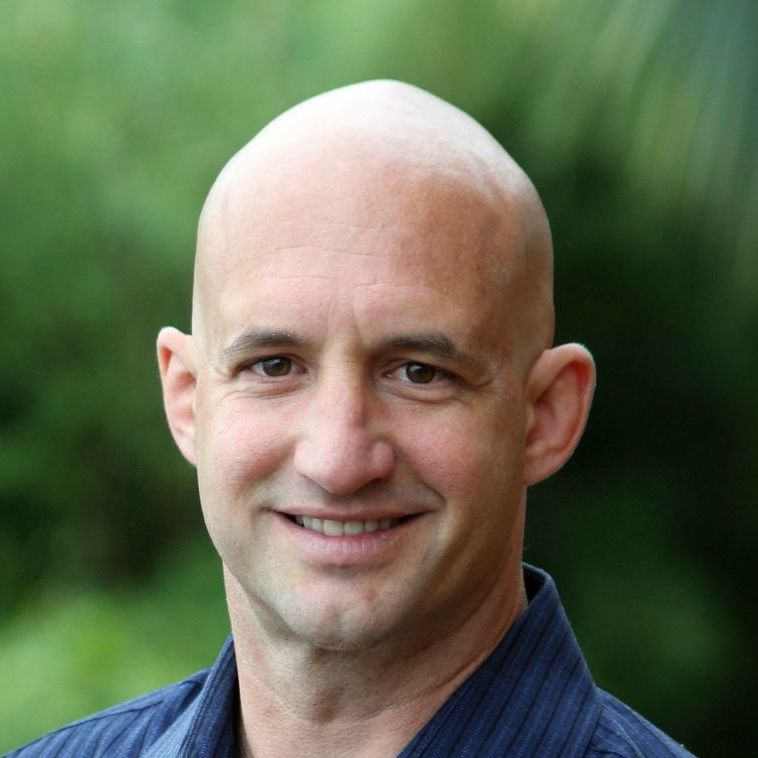
\includegraphics[width=0.7\textwidth]{img/eric-brewer.jpg}\\
             	\vspace{0.3cm}
                Eric Brewer\\
                Professeur à l'université de Berkeley
             \end{center}
        \end{column}
        \begin{column}{0.63\textwidth}
               Selon \textbf{Eric Brewer}, un système informatique ne peut pas garantir simultanément la \textcolor{color-consistency}{\bf consistance}, la \textcolor{color-availability}{\bf disponibilité} et la \textcolor{color-partition}{\bf tolérance aux partitions}. Il faut faire un compromis entre les trois propriétés.
        \end{column}
    \end{columns}

    \note{
        CAP, c’est comme choisir entre : avoir toujours la bonne info (C), toujours un service disponible (A), ou tolérer les pannes (P).
    }


\end{frame}

\begin{frame}{Mais que signifie le théorème CAP ?}
    \begin{itemize}
        \item \textcolor{color-consistency}{\bf Consistency} : toutes les données sont à jour
        \pause
        \item \textcolor{color-availability}{\bf Availability} : toutes les requêtes reçoivent une réponse
        \pause
        \item \textcolor{color-partition}{\bf Partition tolerance} : le système continue de fonctionner malgré les défaillances réseau
    \end{itemize}

    \note{
        \textcolor{color-consistency}{\bf Consistency} : toutes les copies des données sont identiques et à jour. Si une donnée est modifiée, toutes les répliques doivent refléter ce changement immédiatement.

        Un système est cohérent si le client peut interroger n’importe quelle réplique d’un objet à un instant donné, et obtenir à chaque fois le même résultat.

        Pour des raisons d’efficacité, les systèmes distribuées créent et propagent les répliques de manière asynchrone. Il est donc possible qu’un objet ne soit pas cohérent pendant un court instant, le temps que les répliques se fassent.

        De nombreux systèmes \textbf{garantissent ainsi une cohérence à terme} (eventual consistency).


        \textcolor{color-availability}{\bf Availability} : le système répond toujours aux requêtes, même si certaines parties du système sont en panne. Chaque requête reçoit une réponse, mais pas nécessairement la plus récente.

        Un système est disponible à un instant donné si toute requête envoyée au cluster par un client à ce moment est prise en compte. Cela ne signifie pas que la requête est exécutée : elle peut être mise en attente, mais le client sera au moins informé de la prise en compte.

        Mesure de la disponibilité en \%, par exemple avec une \textbf{disponibilité de 99.99\%} : système indisponible pendant au plus 0.01\% du temps. \textbf{Sur un an, cela représente un total cumulé de 53 min.}

        \textcolor{color-partition}{\bf Partition tolerance} : le système continue de \textbf{fonctionner correctement même si des messages sont perdus ou retardés} entre les nœuds du système. Il peut y avoir des partitions réseau, mais le système doit rester opérationnel.

        Par exemple, lorsqu’un nœud du cluster crashe, ou qu’un lien réseau disparaît, mettant une portion entière du cluster hors de portée.

    }

\end{frame}

\begin{frame}{Théorème CAP}

    \begin{figure}[htb]
        \resizebox{!}{0.85\textheight}{
        \begin{tikzpicture}
            % Circle 1: Consistency
            \draw[very thick, color=color-consistency, pattern=north east lines, pattern color=color-consistency] (0,0) circle (3cm);
            \node[fill=color-consistency, text=white, font=\bfseries, rounded corners] at (0,0.5) {Consistency};

            % Circle 2: Availability
            % \fill[pattern=north lines, pattern color=color-availability] (-2.5,-3.25) circle (3cm);
            \draw[very thick, color=color-availability] (-2.1,-3.25) circle (3cm);
            \node[fill=color-availability, text=white, font=\bfseries, rounded corners] at (-2.75,-3.5) {Availability};

            % Circle 3: Partition Tolerance
            % \fill[pattern=north east lines, pattern color=color-partition] (2.5,-3.25) circle (3cm);
            \draw[very thick, color=color-partition] (2.1,-3.25) circle (3cm);
            \node[fill=color-partition, text=white, font=\bfseries, rounded corners, align=left] at (2.75,-3.5) {Partition \\ tolerance};

			\onslide<2->{
	            \node[fill=none, font=\bfseries, text=color-ca] at (-1.4,-1.5) {CA};
	            \node[fill=none, font=\bfseries, text=color-cp] at (1.4,-1.5) {CP};
	            \node[fill=none, font=\bfseries, text=color-ap] at (0,-3.7) {AP};
			}
            \onslide<3->{
                \node[inner sep=0pt] (unicorn) at (0,-2.25) {
\includegraphics[width=1cm]{img/unicorn.png}};
            }
        \end{tikzpicture}
        }
    \end{figure}

    \note{

        \textbf{CA} : un problème sur un des noeuds fait stopper le système

        \textbf{CP} : les données ne sont pas forcément disponibles au moment de la requête

        \textbf{AP} : les données renvoyées ne sont pas toujours cohérentes
    }
\end{frame}

\subsection{ACID vs BASE}

\begin{frame}{ACID}

    Donner définition des propriétés ACID

\end{frame}

\begin{frame}{ACID vs BASE}

    \begin{figure}[htb]
        \centering
        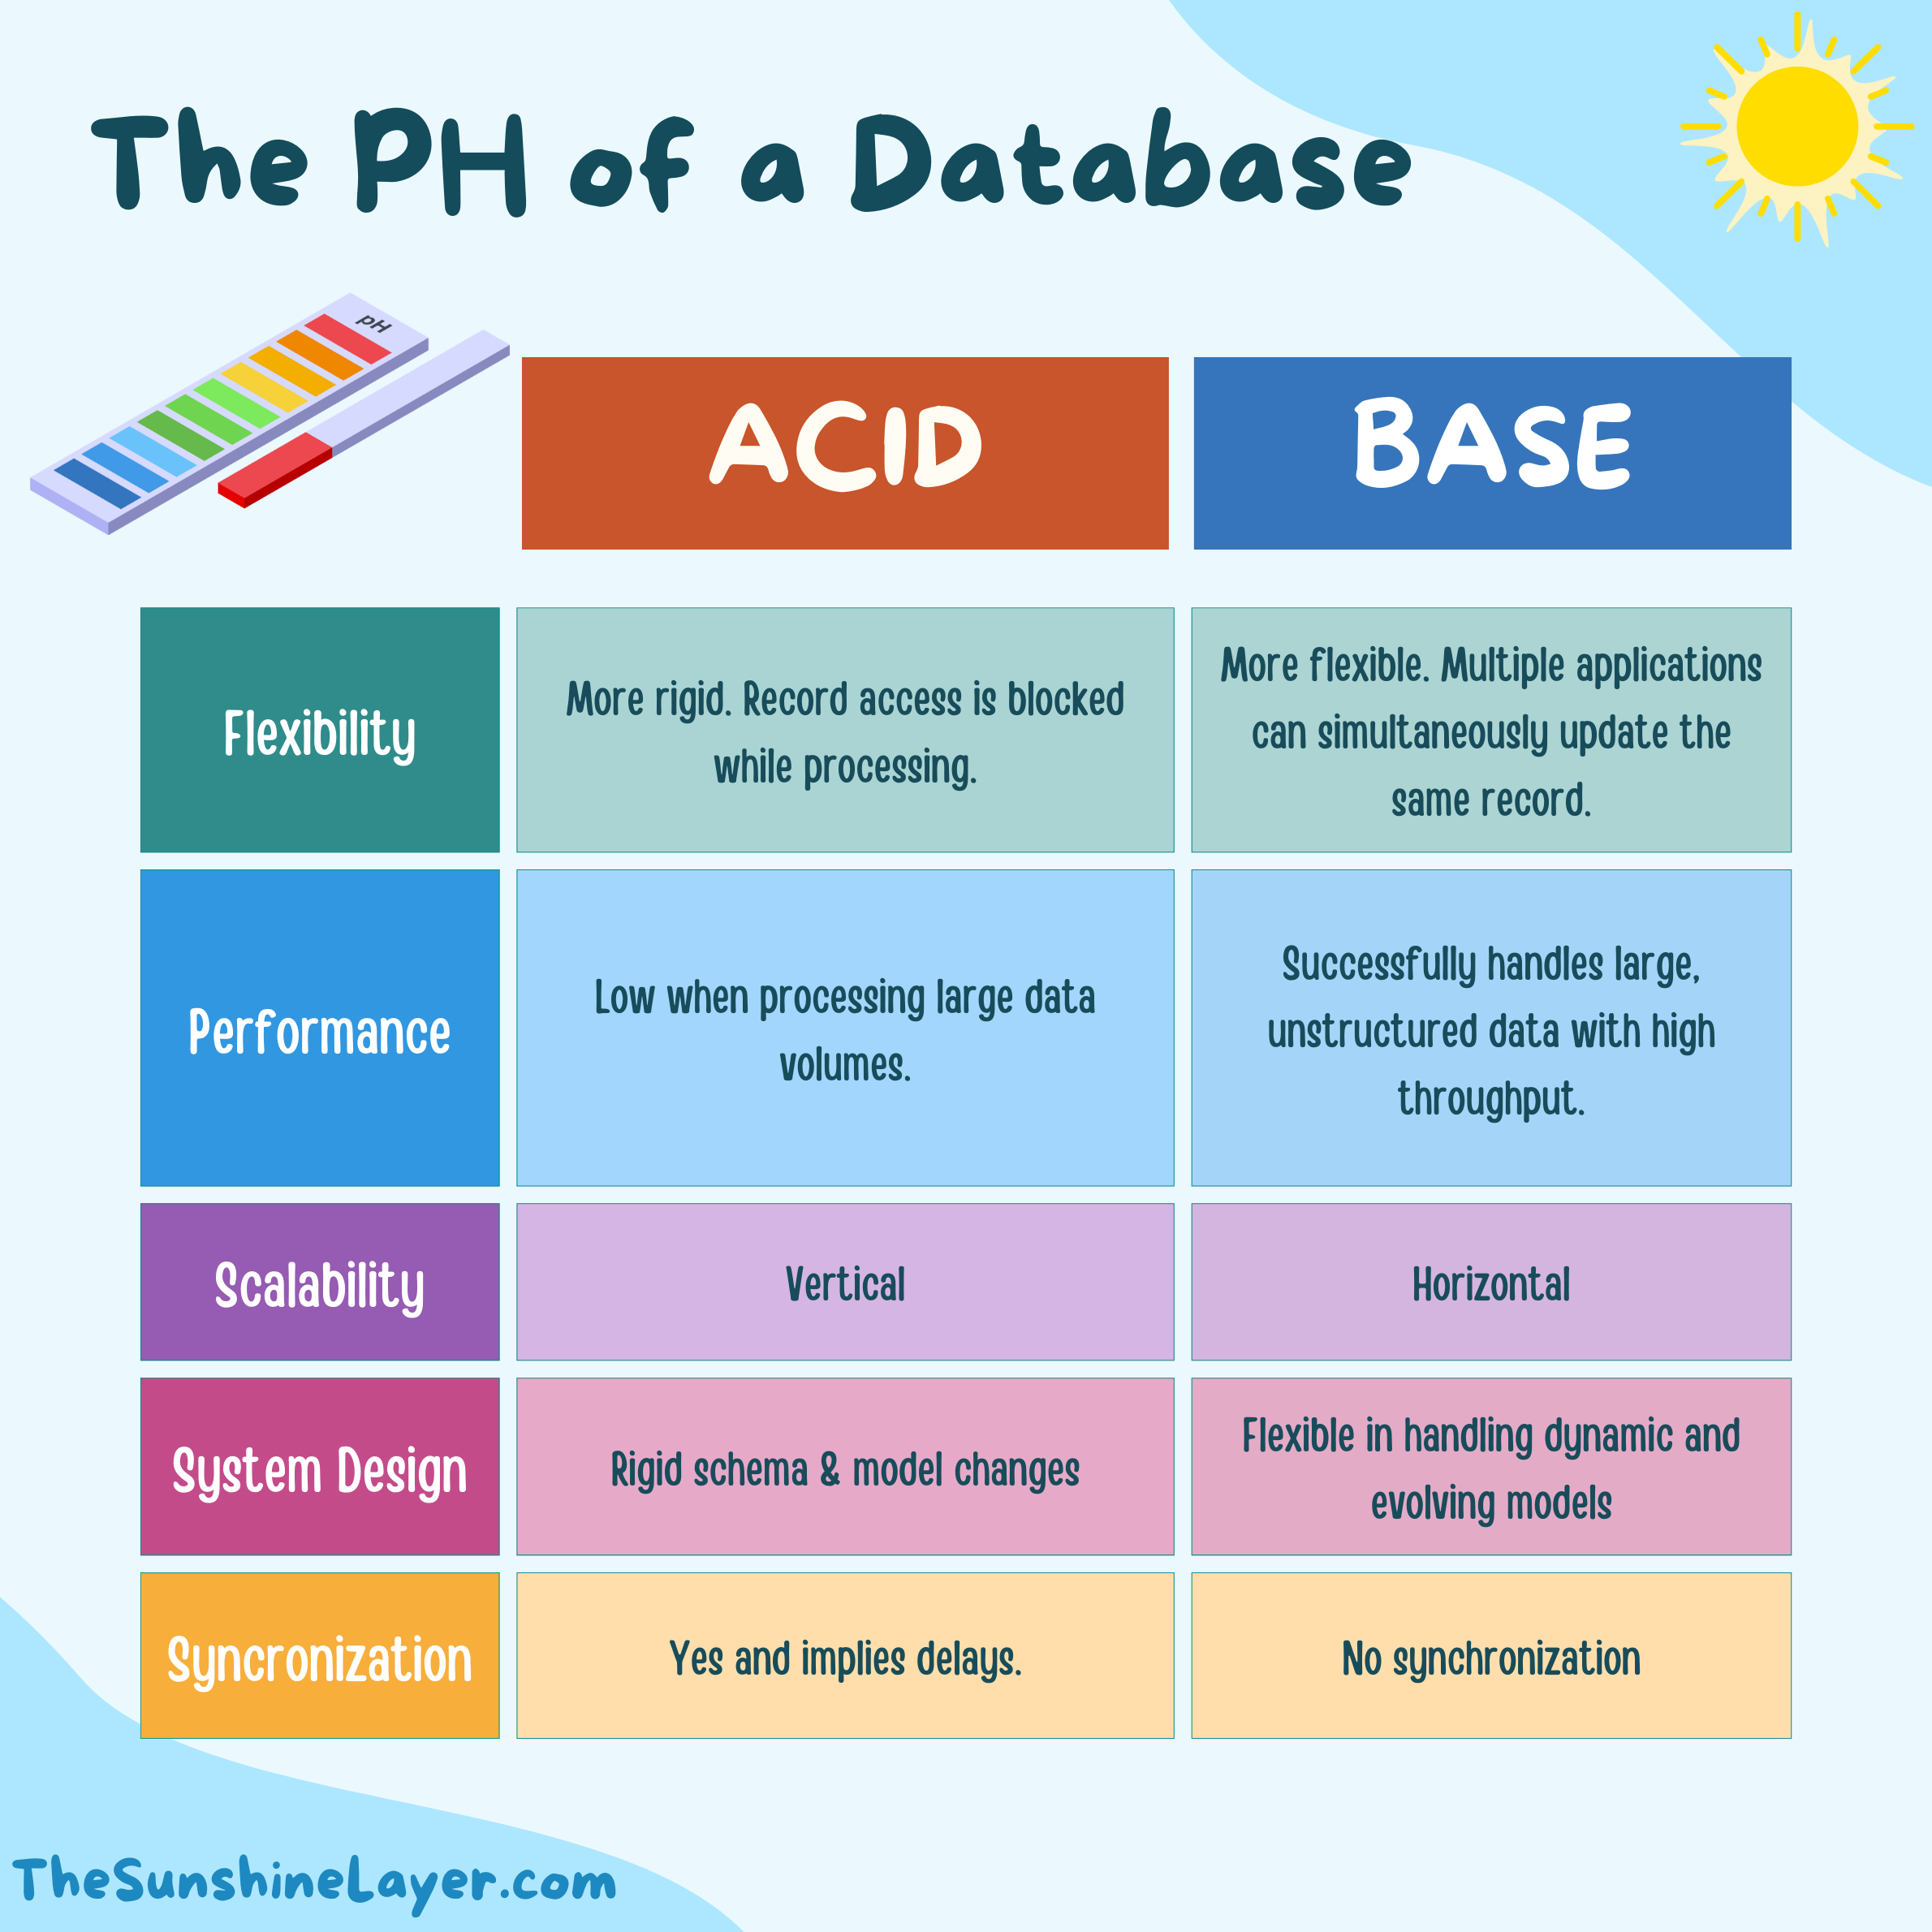
\includegraphics[height=0.9\textheight]{img/acid-vs-base.png}
    \end{figure}

\end{frame}

\begin{frame}{Transactions ACID}

    \begin{itemize}
        \item Atomicité : Toutes les opérations d'une transaction sont exécutées ou aucune
        \item Cohérence : La base de données passe d'un état valide à un autre état valide
        \item Isolation : Les transactions s'exécutent indépendamment les unes des autres
        \item Durabilité : Les modifications sont persistantes
    \end{itemize}


\end{frame}


\begin{frame}{Propriétés BASE}

    \begin{itemize}
        \item Basically Available : Le système est toujours disponible
        \item Soft state : L'état du système peut changer
        \item Eventually consistent : Le système finit par être cohérent
    \end{itemize}

\end{frame}

\subsection{Indexation}

\begin{frame}{Qu'est-ce que l'indexation}

    Définition et examples

\end{frame}

\begin{frame}{Indexation}

    \begin{itemize}
        \item Indexation secondaire
        \item Indexation composite
        \item Indexation géospatiale
    \end{itemize}

\end{frame}

%\subsection{Benchmark}
%
%\begin{frame}
%    Comparaison des performances (latence, débit) entre SQL et NoSQL sur des cas d’usage.
%    Exemple : Benchmark MongoDB vs PostgreSQL pour des requêtes de type "find all users with age > 25".
%    Outils : Utiliser des données réelles (ex : TechEmpower Benchmarks).
%\end{frame}

\begin{frame}{Avantages et inconvénients du NoSQL}

    \pause

    \prosbox{
    \textbf{Avantages}
    \begin{itemize}
        \item Flexibilité du schéma
        \item Scalabilité horizontale
    \end{itemize}
    }

    \note{

        Flexibilité du schéma : pas de structure rigide, adapté aux données non structurées ou évolutives (JSON, documents, graphes...)

        Scalabilité horizontale : conçu pour répartir la charge sur plusieurs serveurs facilement, idéal pour les gros volumes de données

    }

    \vspace{0.5cm}
    \pause

    \consbox{
    \textbf{Inconvénients}
    \begin{itemize}
        \item Consistance limitée
        \item Écosystème et requêtes moins matures
    \end{itemize}
    }

    \note
    {
        Cohérence limitée : privilégie souvent la disponibilité à la cohérence forte (modèle BASE plutôt qu'ACID), ce qui peut poser problème pour les transactions critiques + théorème CAP

        Écosystème et requêtes moins matures : pas de langage standard comme SQL, jointures complexes difficiles, et moins d'outils/expertise disponibles selon la technologie choisie
    }

\end{frame}

\begin{frame}{Quand utiliser une base NoSQL ?}

    \begin{figure}[htb]
        \centering
        \resizebox{\textwidth}{!}{
        \begin{tikzpicture}

            \node[inner sep=0pt, label=below:Big Data] (big-data) at (0,0)
                {\includegraphics[width=.2\textwidth]{img/icon/big-data.png}};

            \node[inner sep=0pt, label=below:Temps réel, right=of big-data, xshift=1cm] (real-time)
                {\includegraphics[width=.2\textwidth]{img/icon/real-time.png}};

            \node[inner sep=0pt, label=below:Données non-structurées, right=of real-time, xshift=1cm] (unstructured)
                {
\includegraphics[width=.2\textwidth]{img/icon/unstructured.png}};
        \end{tikzpicture}
        }
    \end{figure}

    \note{
        À noter que le choix dépend surtout du cas d'usage : NoSQL brille pour le Big Data, le temps réel ou les données semi-structurées, alors que SQL reste préférable pour les données fortement relationnelles nécessitant des garanties transactionnelles strictes.

        \begin{itemize}
            \item Grande quantité de données semi-structurées ou non structurées (logs, réseaux sociaux, IoT, time-based data)
            \item Améliorer les performances d'accès aux données en combinant le traitement de volumes de données plus importants, la réduction des temps de latence et l'amélioration du débit.
        \end{itemize}

        Quelques exemples d'applications qui bénéficient de l'utilisation de bases NoSQL :
        \begin{itemize}
            \item Applications web et mobiles
            \item Big Data et analytics
            \item Gestion de contenu et réseaux sociaux
            \item Internet des objets (IoT)
        \end{itemize}
    }

\end{frame}

\begin{frame}{SQL vs NoSQL expliqué en 4 minutes}
    \centering
    % SQL vs. NoSQL Explained (in 4 Minutes): https://www.youtube.com/watch?v=_Ss42Vb1SU4
    \href{run:/Users/alanna/Documents/Teaching/2026-2027/IUT/NoSQL/Cours/video/nosql.mp4}{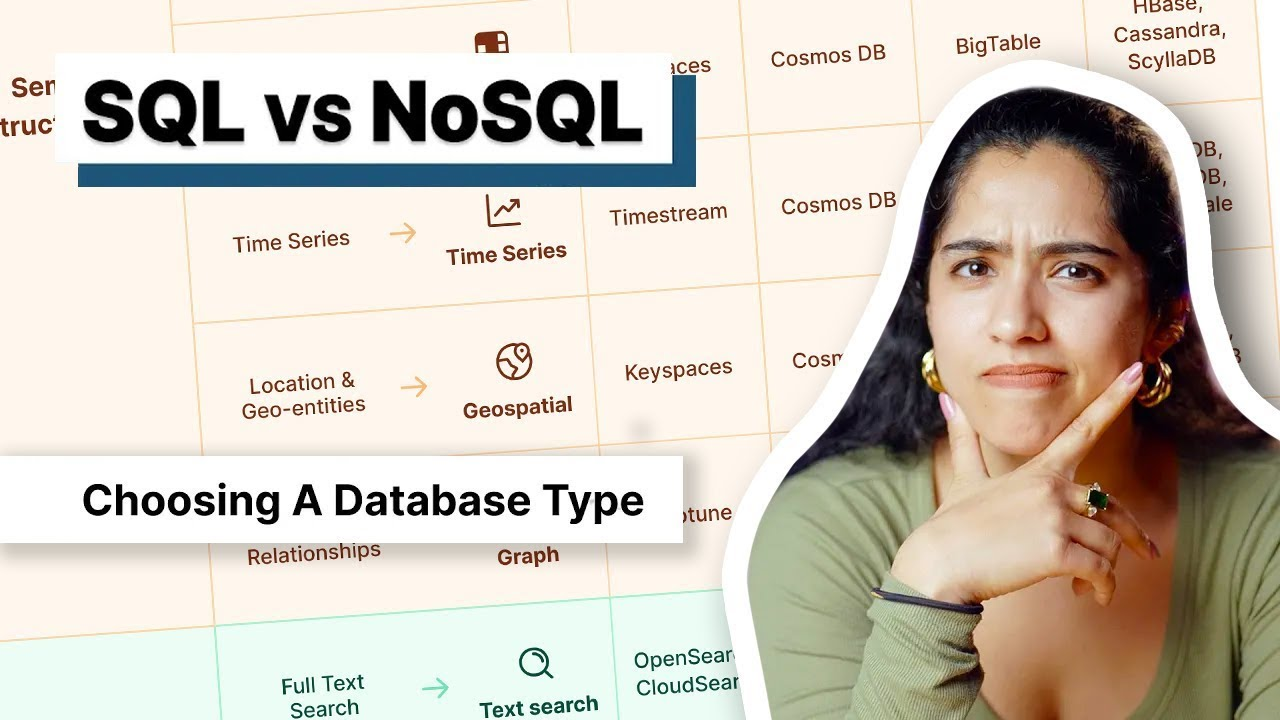
\includegraphics[height=5cm]{img/youtube-thumbnail.jpg}}

\end{frame}


\begin{frame}{Relationnel ou NoSQL ?}


    \textbf{Conception d'un système de réseau social}

    On veut gérer une grande volumétrie de publications. La diffusion de posts auprès de plusieurs utilisateurs peut prendre un certain temps.

    \begin{itemize}
        \item Relationnel
        \item \textcolor<2>{kh-green}{\textbf<2>{NoSQL}}
    \end{itemize}

    \note{
        Étant donné que les données des publications seront principalement des données non structurées (texte/images/vidéos) et que l'on aura besoin d'une évolutivité horizontale (des milliards de publications), on devrait opter pour une base de données NoSQL.
    }

\end{frame}

\begin{frame}{Relationnel ou NoSQL ?}

    \textbf{Conception d'un système de paiement}

    Pour ce système bancaire, il est primordial que les transactions reflètent le compte des client$\cdot$es. Le système ne doit pas créer d'incohérences, ce qui peut entraîner des conséquences indésirables (soldes négatifs) et des client$\cdot$es mécontents.

    \begin{itemize}
        \item \textcolor<2>{kh-green}{\textbf<2>{Relationnel}}
        \item NoSQL
    \end{itemize}

    \note{
        Étant donné que les données sont structurées et que plusieurs utilisateurs n'ont pas besoin de consulter une seule transaction, il est préférable d'utiliser une base de données relationnelle.
    }


\end{frame}

\begin{frame}[standout]

    Avez-vous été attentifs ?

    À vous de jouer !

\end{frame}

{
\setbeamercovered{transparent}

\begin{frame}{Q1}

    \textbf{Qu'est-ce que le NoSQL ?}

    \begin{itemize}
        \item \uncover<1>{\textcolor{kh-red}{Langage de programmation de manipulation de bases de données relationnelles}}
        \item \textbf<2>{\textcolor{kh-blue}{Bases de données non relationnelles conçues pour des données distribuées et volumineuses}}
        \item \uncover<1>{\textcolor{kh-green}{Protocole de communication pour les réseaux informatiques}}
        \item \uncover<1>{\textcolor{kh-yellow}{Système de gestion de bases de données exclusivement destiné au traitement des transactions}}
    \end{itemize}

\end{frame}

\begin{frame}{Q2}

    \textbf{Quelle est la principale utilité du partitionnement dans les bases de données NoSQL ?}

    \begin{itemize}
        \item \textbf<2>{\textcolor{kh-red}{Il améliore les performances en répartissant les données sur plusieurs nœuds}}
        \item \uncover<1>{\textcolor{kh-blue}{Il sert uniquement à réduire la taille physique des fichiers de la base de données sur le disque dur}}
        \item \uncover<1>{\textcolor{kh-green}{Il permet de crypter automatiquement les données pour renforcer la sécurité des informations stockées}}
        \item \uncover<1>{\textcolor{kh-yellow}{Il est utilisé pour convertir les bases de données NoSQL en bases de données relationnelles afin de supporter le langage SQL}}
    \end{itemize}

\end{frame}

\begin{frame}{Q2}

    \textbf{Quelle est la principale caractéristique des bases de données NoSQL ?}

    \begin{itemize}
        \item \textbf<2>{\textcolor{kh-red}{Propriétés BASE}}
        \item \uncover<1>{\textcolor{kh-blue}{Transactions ACID}}
        \item \uncover<1>{\textcolor{kh-green}{Langage SQL}}
        \item \uncover<1>{\textcolor{kh-yellow}{Open Database Connectivity}}
    \end{itemize}

\end{frame}

\begin{frame}{Q3}

    \textbf{Quels sont les mécanismes pour assurer disponibilité et tolérance aux pannes dans un environnement distribué ?}

    \begin{itemize}
        \item \textbf<2>{\textcolor{kh-red}{Réplication des données}}
        \item \textbf<2>{\textcolor{kh-blue}{Sharding}}
        \item \uncover<1>{\textcolor{kh-green}{Transactions ACID strictes}}
        \item \textbf<2>{\textcolor{kh-yellow}{Cohérence éventuelle}}
    \end{itemize}

\end{frame}

\begin{frame}{Q4}

    \textbf{Que signifient les initiales du théorème CAP ?}

    \begin{itemize}
        \item \uncover<1>{\textcolor{kh-red}{Complexity, Accuracy, Performance}}
        \item \uncover<1>{\textcolor{kh-blue}{Centralized Access Protocol}}
        \item \textbf<2>{\textcolor{kh-green}{Consistency, Availability, Partition Tolerance}}
        \item \uncover<1>{\textcolor{kh-yellow}{Consistency, Availability, Performance}}
    \end{itemize}

\end{frame}

%\begin{frame}
%
%    Ajouter des questions ouvertes (ex : "Proposez une base NoSQL adaptée à un système de recommandation de films").
%    Utiliser des cas réels (ex : "Quel type de base utiliseriez-vous pour stocker les logs d’un site web ?").
%
%\end{frame}

%\begin{frame}{Q5}
%
%    \textbf{}
%
%    \begin{itemize}
%        \item \uncover<1>{\textcolor{kh-red}{}}
%        \item \uncover<1>{\textcolor{kh-blue}{}}
%        \item \textbf<2>{\textcolor{kh-green}{}}
%        \item \uncover<1>{\textcolor{kh-yellow}{}}
%    \end{itemize}
%
%\end{frame}
%
%\begin{frame}{Q6}
%
%    \textbf{}
%
%    \begin{itemize}
%        \item \uncover<1>{\textcolor{kh-red}{}}
%        \item \uncover<1>{\textcolor{kh-blue}{}}
%        \item \textbf<2>{\textcolor{kh-green}{}}
%        \item \uncover<1>{\textcolor{kh-yellow}{}}
%    \end{itemize}
%
%\end{frame}
%
%\begin{frame}{Q7}
%
%    \textbf{}
%
%    \begin{itemize}
%        \item \uncover<1>{\textcolor{kh-red}{}}
%        \item \uncover<1>{\textcolor{kh-blue}{}}
%        \item \textbf<2>{\textcolor{kh-green}{}}
%        \item \uncover<1>{\textcolor{kh-yellow}{}}
%    \end{itemize}
%
%\end{frame}
%
%\begin{frame}{Q8}
%
%    \textbf{}
%
%    \begin{itemize}
%        \item \uncover<1>{\textcolor{kh-red}{}}
%        \item \uncover<1>{\textcolor{kh-blue}{}}
%        \item \textbf<2>{\textcolor{kh-green}{}}
%        \item \uncover<1>{\textcolor{kh-yellow}{}}
%    \end{itemize}
%
%\end{frame}
%
%\begin{frame}{Q9}
%
%    \textbf{}
%
%    \begin{itemize}
%        \item \uncover<1>{\textcolor{kh-red}{}}
%        \item \uncover<1>{\textcolor{kh-blue}{}}
%        \item \textbf<2>{\textcolor{kh-green}{}}
%        \item \uncover<1>{\textcolor{kh-yellow}{}}
%    \end{itemize}
%
%\end{frame}
%
%\begin{frame}{Q10}
%
%    \textbf{}
%
%    \begin{itemize}
%        \item \uncover<1>{\textcolor{kh-red}{}}
%        \item \uncover<1>{\textcolor{kh-blue}{}}
%        \item \textbf<2>{\textcolor{kh-green}{}}
%        \item \uncover<1>{\textcolor{kh-yellow}{}}
%    \end{itemize}
%
%\end{frame}

}


\section{Typologie des bases\\de données NoSQL}

\begin{frame}{Ecosystème NoSQL}
    \begin{figure}[htb]
        \centering
        \resizebox{0.95\textwidth}{!}{
        \begin{tikzpicture}
            \node[minimum width=3cm, minimum height=2cm] at (0, 0) {\includesvg[height=1cm]{img/db/redis.svg}};
            \node[minimum width=3cm, minimum height=2cm] at (1.5, -1) {
\includegraphics[height=0.8cm]{img/db/oracle-nosql.png}};
            \node[minimum width=3cm, minimum height=2cm] at (4, -0.5) {\includesvg[height=1cm]{img/db/couchdb.svg}};
            \node[minimum width=3cm, minimum height=2cm] at (6, 0.2) {\includesvg[height=1.3cm]{img/db/aws-documentdb.svg}};
            \node[minimum width=3cm, minimum height=2cm] at (0, -2) {\includesvg[height=0.8cm]{img/db/couchbase.svg}};
            \node[minimum width=3cm, minimum height=2cm] at (0.5, -6) {
\includegraphics[height=1cm]{img/db/aws-dynamodb.png}};
            \node[minimum width=3cm, minimum height=2cm] at (2, -3.5) {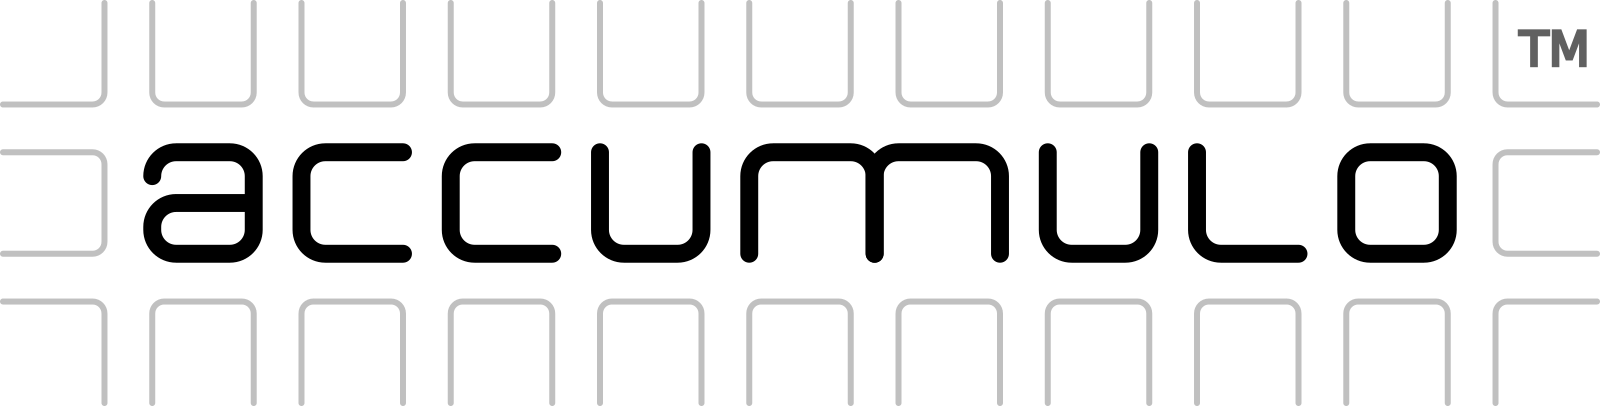
\includegraphics[height=1cm]{img/db/accumulo.png}};
            \node[minimum width=3cm, minimum height=2cm] at (2, -4.8) {\includesvg[height=1cm]{img/db/mongodb.svg}};
            \node[minimum width=3cm, minimum height=2cm] at (4.5, -4.8) {
\includegraphics[height=1.2cm]{img/db/scylla-db.png}};
            \node[minimum width=3cm, minimum height=2cm] at (6, -2) {\includesvg[height=0.6cm]{img/db/ravendb.svg}};
            \node[minimum width=3cm, minimum height=2cm] at (-1.5, -3.2) {
\includegraphics[height=1cm]{img/db/hypertable.png}};
            \node[minimum width=3cm, minimum height=2cm] at (7.5, -5.5) {\includesvg[height=1cm]{img/db/firestore.svg}};
            \node[minimum width=3cm, minimum height=2cm] at (3, -2.3) {\includesvg[height=0.7cm]{img/db/riak.svg}};
            \node[minimum width=3cm, minimum height=2cm] at (-2, -6) {\includesvg[height=1cm]{img/db/cassandra.svg}};
            \node[minimum width=3cm, minimum height=2cm] at (7, -4) {\includesvg[height=1cm]{img/db/hbase.svg}};
            \node[minimum width=3cm, minimum height=2cm] at (-1.5, -1) {
\includegraphics[height=0.8cm]{img/db/gcp-bigtable.png}};
            \node[minimum width=3cm, minimum height=2cm] at (3, -6) {\includesvg[height=0.7cm]{img/db/druid.svg}};
            \node[minimum width=3cm, minimum height=2cm] at (-1.3, -4.5) {\includesvg[height=1cm]{img/db/neo4j.svg}};
            \node[minimum width=3cm, minimum height=2cm] at (7, -1) {\includesvg[height=1cm]{img/db/arangodb.svg}};
            \node[minimum width=3cm, minimum height=2cm] at (7, -3) {\includesvg[height=1cm]{img/db/orientdb.svg}};
            \node[minimum width=3cm, minimum height=2cm] at (6, -5.5) {
\includegraphics[height=1.3cm]{img/db/aws-neptune.png}};
            \node[minimum width=3cm, minimum height=2cm] at (7, -7) {\includesvg[height=1cm]{img/db/memcached.svg}};
        \end{tikzpicture}
        }
    \end{figure}
\end{frame}


\begin{frame}{Typologie des bases de données NoSQL}

    \begin{figure}
        \centering
        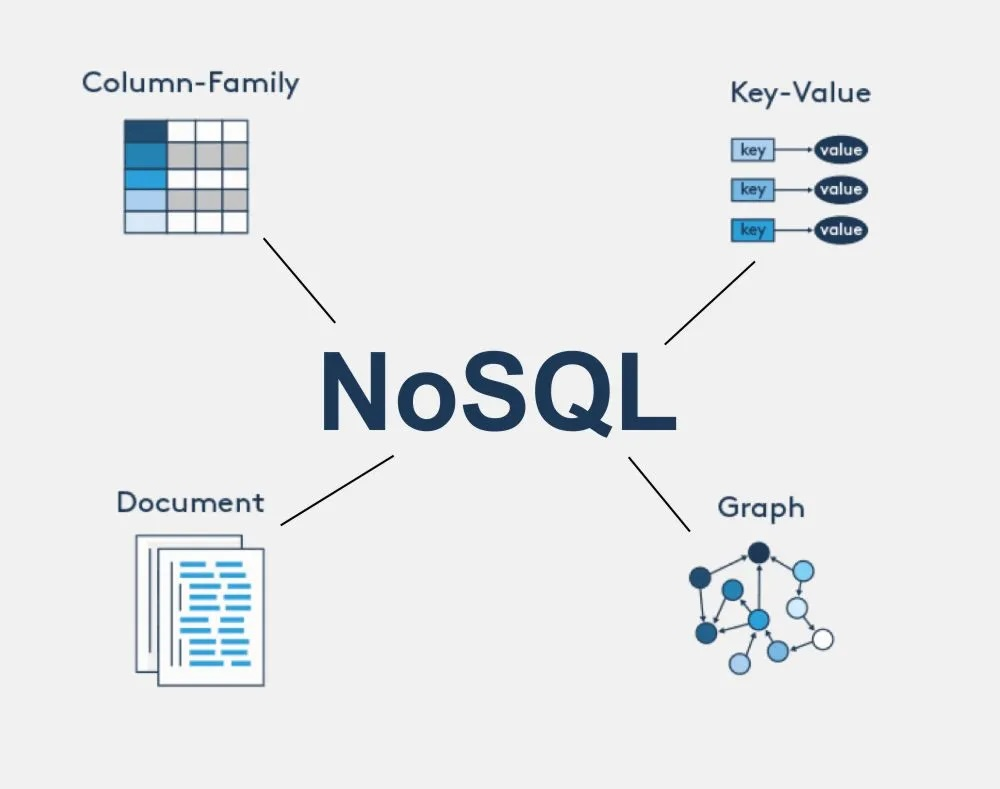
\includegraphics[width=0.8\textwidth]{img/nosql-database-types.jpg}
    \end{figure}

\end{frame}

% ------------------------------------------------------------------------------------------------------------------------------------------------------------------------

\begin{frame}[standout]

    Bases de données clé-valeur

\end{frame}

\begin{frame}
    "Une base clé-valeur, c’est comme un dictionnaire : tu cherches un mot (clé) et tu obtiens sa définition (valeur)."
\end{frame}

\begin{frame}{Caractéristiques des bases de données clé-valeur}

    \begin{definitionbox}
        Dans une base de données clé-valeur, les données sont stockées sous forme de \textbf{paires de clés uniques et de valeurs} correspondantes.

        La clé agit comme un \textbf{identifiant unique}, et la valeur peut être de tout type (chaîne de caractères, JSON, binaire, etc.).
    \end{definitionbox}

    \begin{noteblock}
        \begin{itemize}
            \item Très scalable avec une structure simple.
            \item Pas de schéma ou de structure rigide ; stockage de données flexible.
        \end{itemize}
        % $\Longrightarrow$ Idéal pour stocker de grandes quantités de données avec une complexité relationnelle minimale.
        $\hookrightarrow$ Idéal pour stocker de grandes quantités de données avec une complexité relationnelle minimale.
    \end{noteblock}
\end{frame}

\begin{frame}{Comment fonctionnent les bases de données clé-valeur ?}

    \begin{figure}
        \centering
        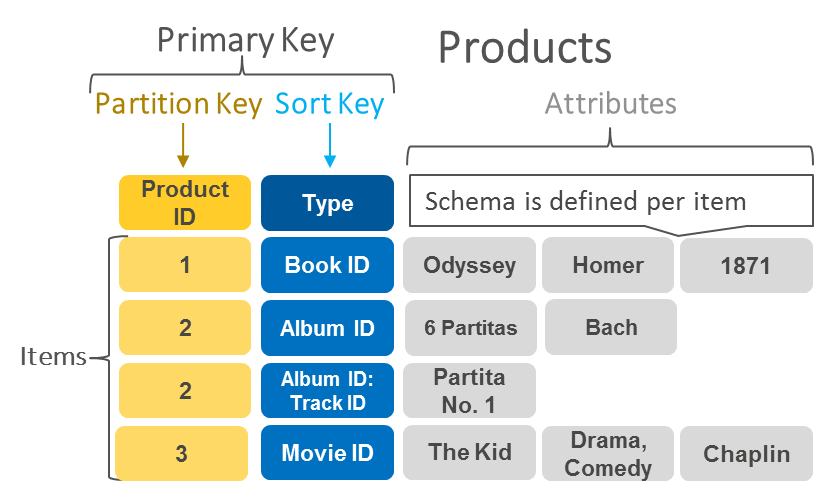
\includegraphics[width=0.8\textwidth]{img/key-value-database.png}
    \end{figure}

\end{frame}

\begin{frame}{Bases de données clé-valeur}
    \begin{figure}[htb]
        \centering
        \begin{tikzpicture}
            \node[minimum width=3cm, minimum height=2cm] at (0, 0) {\includesvg[height=1cm]{img/db/redis.svg}};
            \node[minimum width=3cm, minimum height=2cm] at (0, -2) {\includesvg[height=1cm]{img/db/riak.svg}};
            \node[minimum width=3cm, minimum height=2cm] at (4, 0) {\includesvg[height=1cm]{img/db/memcached.svg}};
            \node[minimum width=3cm, minimum height=2cm] at (4, -2) {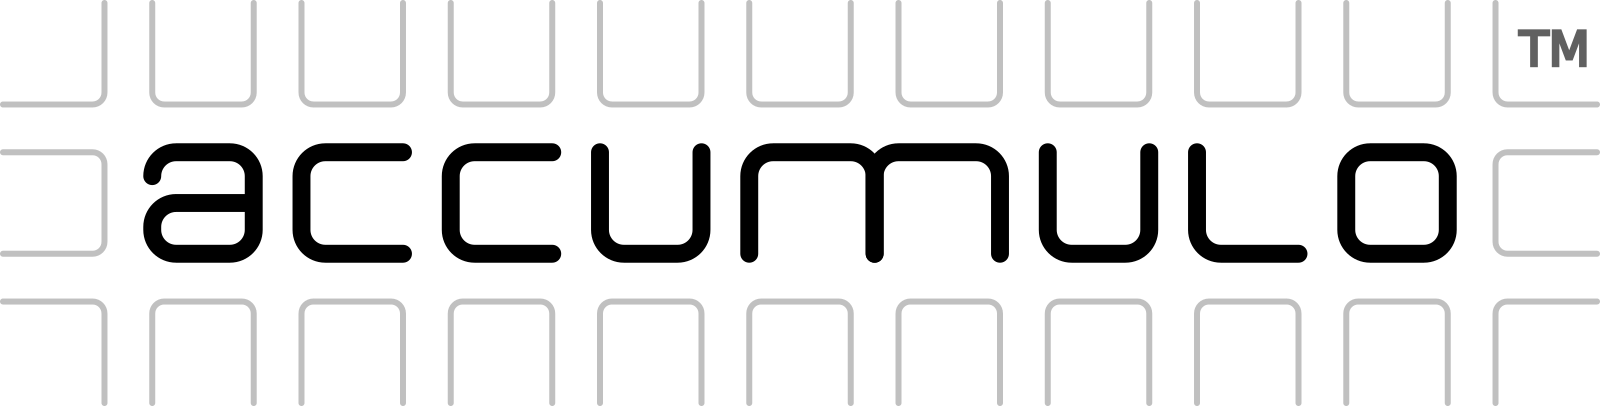
\includegraphics[height=1cm]{img/db/accumulo.png}};
            \node[minimum width=3cm, minimum height=2cm] at (0, -4) {
\includegraphics[height=1cm]{img/db/aws-dynamodb.png}};
            \node[minimum width=3cm, minimum height=2cm] at (4, -4) {
\includegraphics[height=1cm]{img/db/oracle-nosql.png}};
        \end{tikzpicture}
    \end{figure}
\end{frame}


\begin{frame}{Cas d'usages des bases de données clé-valeur}
    % Gestion de session
    % Une application orientée session telle qu'une application web ouvre une session lorsqu'un utilisateur se connecte à une application,
    % puis ferme la session lorsque l'utilisateur se déconnecte ou lorsque la session expire.
    % Pendant cette période, l'application stocke tous les attributs de la session utilisateur dans la mémoire principale ou dans une base de données.
    % Les données de session peuvent inclure des informations sur le profil d'utilisateur, des messages, des données et des thèmes personnalisés,
    % des recommandations, des promotions ciblées et des remises.
    % Chaque session utilisateur possède un identifiant unique. Les données de session sont uniquement interrogées par une clé primaire.
    % Ainsi, un magasin clé-valeur rapide est idéal dans ce contexte. En général, les frais généraux par page liés aux bases de données clé-valeur
    % sont inférieurs à ceux associés aux bases de données relationnelles.

    % Panier d'achat
    % Un site Web d'e-commerce peut recevoir des milliards de commandes en quelques secondes pendant la période des achats de Noël.
    % Les bases de données clé-valeur peuvent gérer la mise à l'échelle de grandes quantités de données et de grands volumes de changements d'état
    % tout en répondant aux besoins de millions d'utilisateurs simultanés grâce à un traitement et à un stockage distribués.
    % Le stockage de données clé-valeur intègre également une capacité de redondance, ce qui lui permet de gérer la perte de nœuds de stockage.

    % Moteur de stockage des métadonnées
    % Votre stockage clé-valeur peut servir de couche de stockage sous-jacente pour des niveaux d'accès aux données plus élevés.
    % Par exemple, vous pouvez mettre à l'échelle le débit et la simultanéité pour les charges de travail multimédias et de divertissement
    % telles que le streaming vidéo en temps réel et le contenu interactif. Vous pouvez également créer votre plateforme de jeu avec les données
    % des joueurs, l'historique des sessions et les tableaux de classement pour des millions d'utilisateurs simultanés.

    % Mise en cache
    % Vous pouvez utiliser une base de données clé-valeur pour stocker temporairement des données afin de les récupérer plus rapidement.
    % Par exemple, les applications de réseaux sociaux peuvent stocker des données fréquemment consultées, telles que le contenu des fils d'actualités.
    % Les systèmes de mise en cache des données en mémoire utilisent également le stockage clé-valeur pour accélérer les réponses des applications.

    \begin{itemize}
        \item \textbf{Stockage de sessions et profils d'utilisateurs}\\
        $\hookrightarrow$ Chaque utilisateur est référencé par une clé qui permet d'accéder à ses informations.
        \vspace{0.3cm}

        \item \textbf{Paniers d'achats dans les applications de commerce électronique}\\
        $\hookrightarrow$ Gestion des commandes lors des soldes et de l'évolution de leur statut.
        \vspace{0.3cm}

        \item \textbf{Moteur de stockage des métadonnées}\\
        $\hookrightarrow$ Pour une plateforme de jeu, cela permet d'accéder aux données des joueurs, l'historique des sessions et les tableaux de classement pour des millions d'utilisateurs simultanés.
        \vspace{0.3cm}

        \item \textbf{Systèmes de cache (ex. : Redis, Memcached)}\\
        $\hookrightarrow$ Les applications de réseaux sociaux peuvent stocker des données fréquemment consultées, telles que le contenu des fils d'actualités.
    \end{itemize}
\end{frame}

\begin{frame}{Avantages et inconvénients des bases de données clé-valeur}
    \vfill
    \prosbox{
        \textbf{Avantages}
        \begin{itemize}
            \item Lectures et écritures extrêmement rapides grâce à l'accès direct par clé.
            \item Scalabilité horizontale facile pour de grands ensembles de données.
        \end{itemize}
    }
    \vfill
    \pause
    \consbox{
        \textbf{Inconvénients}
        \begin{itemize}
            \item Absence de requêtes complexes.
            \item Mauvaise gestion du schéma.
        \end{itemize}
    }
    \vfill
\end{frame}


\begin{frame}{Focus sur Redis}

\end{frame}

\begin{frame}[standout]

    Bases de données document

\end{frame}

\begin{frame}{Caractéristiques des bases de données document}

    \begin{definitionbox}
        Dans une base de données orientée document, les données sont stockées sous forme de \textbf{documents} structurés, généralement au format \textbf{JSON}, \textbf{BSON}, ou \textbf{XML}.

        Chaque document représente un enregistrement, ce qui permet de stocker des données hiérarchiques et complexes.
    \end{definitionbox}

    \begin{noteblock}
        \begin{itemize}
            \item Très flexible : chaque document peut avoir une structure différente.
            \item Capable de stocker des données complexes et imbriquées.
        \end{itemize}
        $\hookrightarrow$ Idéal pour des applications nécessitant un modèle de données flexible et des mises à jour fréquentes.
    \end{noteblock}
\end{frame}

\begin{frame}{Bases de données document}
    \begin{figure}[htb]
        \centering
        \begin{tikzpicture}
            \node[minimum width=3cm, minimum height=2cm] at (0, 0) {\includesvg[height=1cm]{img/db/mongodb.svg}};
            \node[minimum width=3cm, minimum height=2cm] at (4, 0) {\includesvg[height=1cm]{img/db/couchdb.svg}};
            \node[minimum width=3cm, minimum height=2cm] at (0, -2) {\includesvg[height=0.7cm]{img/db/couchbase.svg}};
            \node[minimum width=3cm, minimum height=2cm] at (4, -2) {\includesvg[height=0.6cm]{img/db/ravendb.svg}};
            \node[minimum width=3cm, minimum height=2cm] at (0, -4) {\includesvg[height=1.3cm]{img/db/aws-documentdb.svg}};
            \node[minimum width=3cm, minimum height=1cm,label=below:Firestore] at (4, -4) {\includesvg[height=1cm]{img/db/firestore.svg}};
        \end{tikzpicture}
    \end{figure}
\end{frame}

\begin{frame}[fragile]{Exemple de document JSON}

\begin{minted}[fontsize={\fontsize{6.7}{7.7}\selectfont}]{json}
[
    {
        "title": "Mamma Mia!",
        "year" : 2008,
        "cast" : {
            "director" : "Phyllida Lloyd",
            "actors" : ["Meryl Streep", "Pierce Brosnan","Amanda Seyfried"]
        },
        "rating" : 6.4,
        "plot" : "The story of a bride-to-be trying to find her real father told
using hit songs by the popular '70s group ABBA."
    },
    {
        "title": "Inception",
        "year" : 2010,
        "rating" : 8.8,
        "genres" : ["Action", "Adventure", "Sci-Fi"],
        "plot" : "A thief who steals corporate secrets through the use of dream-sharing
technology is given the inverse task of planting an idea into the mind of a CEO."
    }
]
\end{minted}

\end{frame}

\begin{frame}{Comment fonctionnent les bases de données document ?}

    \begin{figure}
        \centering
        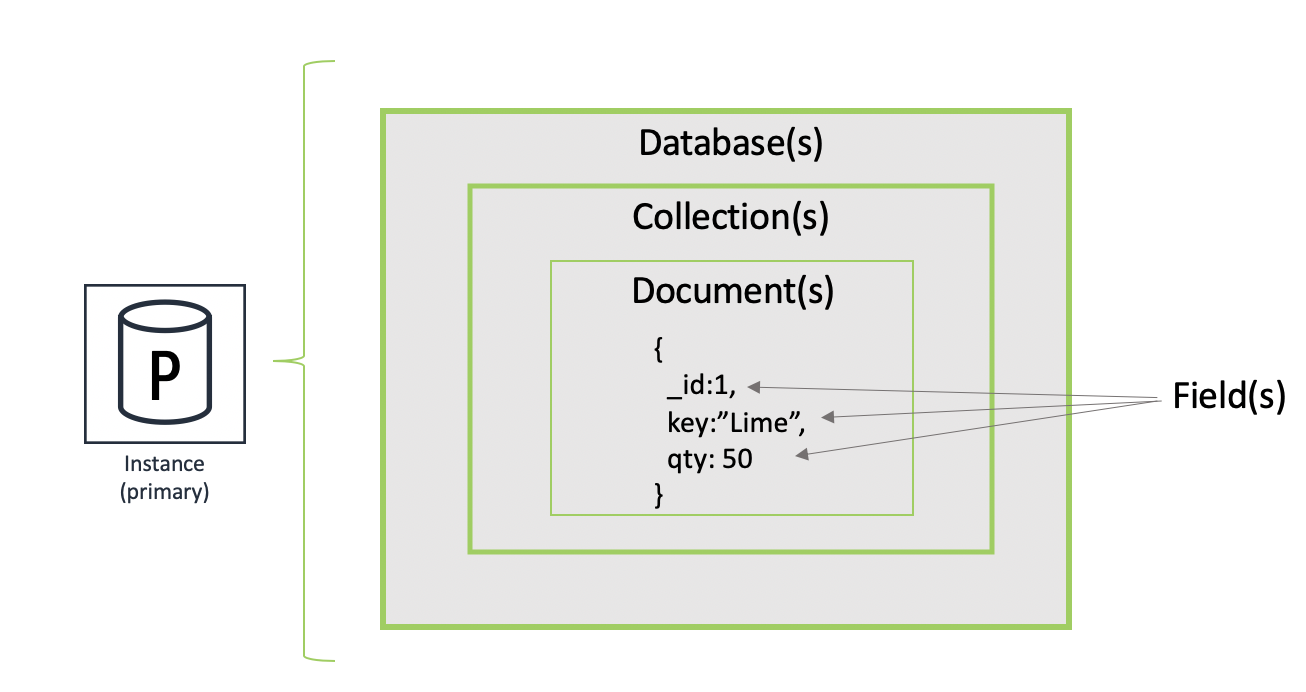
\includegraphics[width=0.8\textwidth]{img/json-document-database.png}
    \end{figure}

\end{frame}


\begin{frame}{Comment fonctionnent les bases de données document ?}

    \textbf{TODO : remplacer l'image par un filtrage sur les données de l'exemple JSON de l'exemple précédent.}

    \begin{figure}
        \centering
        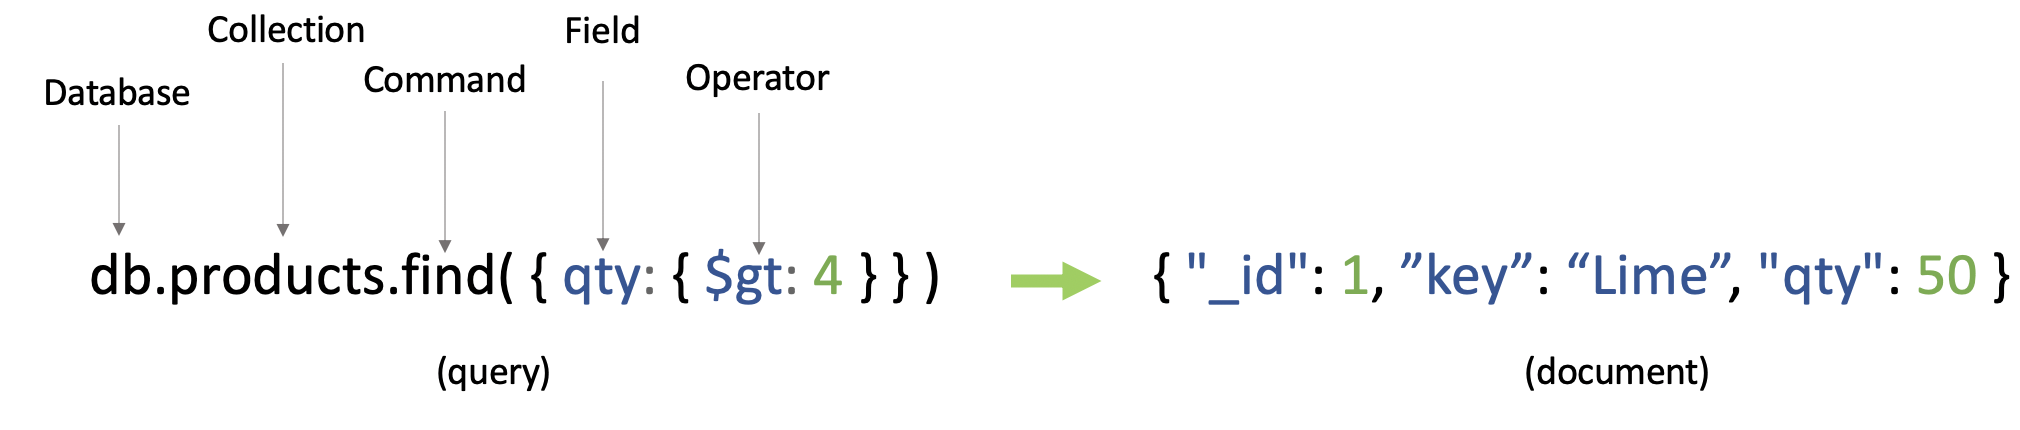
\includegraphics[width=0.8\textwidth]{img/json-database-query.png}
    \end{figure}

\end{frame}

\begin{frame}{Cas d'usages des bases de données document}

\begin{itemize}
    \item \textbf{Gestion du contenu sur les réseaux sociaux}\\
    $\hookrightarrow$ L'activité de chaque utilisateur est stockée sous forme d'un document contenant des informations imbriquées telles que les posts, commentaires, et connexions.
    \vspace{0.3cm}

    \item \textbf{Plateformes de gestion de contenu (CMS)}\\
    $\hookrightarrow$ Stockage de documents flexibles qui contiennent des informations sur des articles de blog, des images, des métadonnées, etc.
    \vspace{0.3cm}

    \item \textbf{Gestion des capteurs}\\
    $\hookrightarrow$ L'Internet des objets (IoT) permet de collecter un grand volume de données brutes à partir de capteurs (données non structurées et évolutives).
\end{itemize}
\end{frame}

% Gestion de contenu
% Une base de données document est un excellent choix pour les applications de gestion de contenu comme les blogs et les plateformes vidéo.
% Avec une base de données document, chaque entité que suit l'application peut être stockée comme un document unique.
% La base de données document est plus intuitive pour qu'un développeur puisse mettre à jour une application à mesure que les exigences évoluent.
% De plus, si le modèle de données doit être modifié, seuls les documents concernés doivent être mis à jour.
% Aucun schéma de mise à jour ou interruption de la base de données n'est nécessaire pour effectuer les modifications.

% Catalogues
% Les bases de données de documents sont un bon moyen de stocker des informations sur les catalogues.
% Par exemple, dans une application d'e-commerce, des produits différents ont souvent des attributs différents.
% Gérer des milliers d'attributs dans des bases de données relationnelles n'est pas efficace, et cela nuit aux performances de lecture.
% En utilisant une base de données document, les attributs de chaque produit peuvent être décrits dans un seul document pour une gestion aisée
% et une vitesse de lecture supérieure. Vous pouvez modifier les attributs d'un produit sans craindre de changer ceux d'un autre produit.

% Gestion des capteurs
% L'Internet des objets (IoT) permet aux entreprises de collecter régulièrement des données à partir d'appareils intelligents tels que des
% capteurs et des compteurs. Les données des capteurs arrivent généralement sous la forme d'un flux continu de valeurs variables.
% En raison de problèmes de latence, certains objets de données peuvent être incomplets, dupliqués ou manquants.
% En outre, vous devez collecter un volume important de données avant de pouvoir les filtrer ou les résumer à des fins d'analyse.
% Les magasins de documents sont plus pratiques dans ce cas. Vous pouvez rapidement stocker les données des capteurs telles quelles,
% sans avoir à les nettoyer ou à les rendre conformes à des schémas prédéterminés. Vous pouvez également les mettre à l'échelle selon vos
% besoins et supprimer des documents entiers une fois les analyses effectuées.

\begin{frame}{Avantages et inconvénients des bases de données document}
\vfill
\prosbox{
    \textbf{Avantages}
    \begin{itemize}
        \item Grande flexibilité dans le schéma, chaque document peut avoir une structure différente.
        \item Bonne gestion des données hiérarchiques ou imbriquées.
        \item Scalabilité horizontale facile grâce à la partition des documents.
    \end{itemize}
}
\vfill
\pause
\consbox{
    \textbf{Inconvénients}
    \begin{itemize}
        \item Performances limitées pour des requêtes complexes ou des jointures entre documents.
        \item Les mises à jour simultanées de documents imbriqués peuvent être plus complexes à gérer.
    \end{itemize}
}
\vfill
\end{frame}

\subsection{Flexibilité du schéma}

\begin{frame}{Quelle flexibilité de schéma ?}

    \begin{figure}[htb]
        \centering
        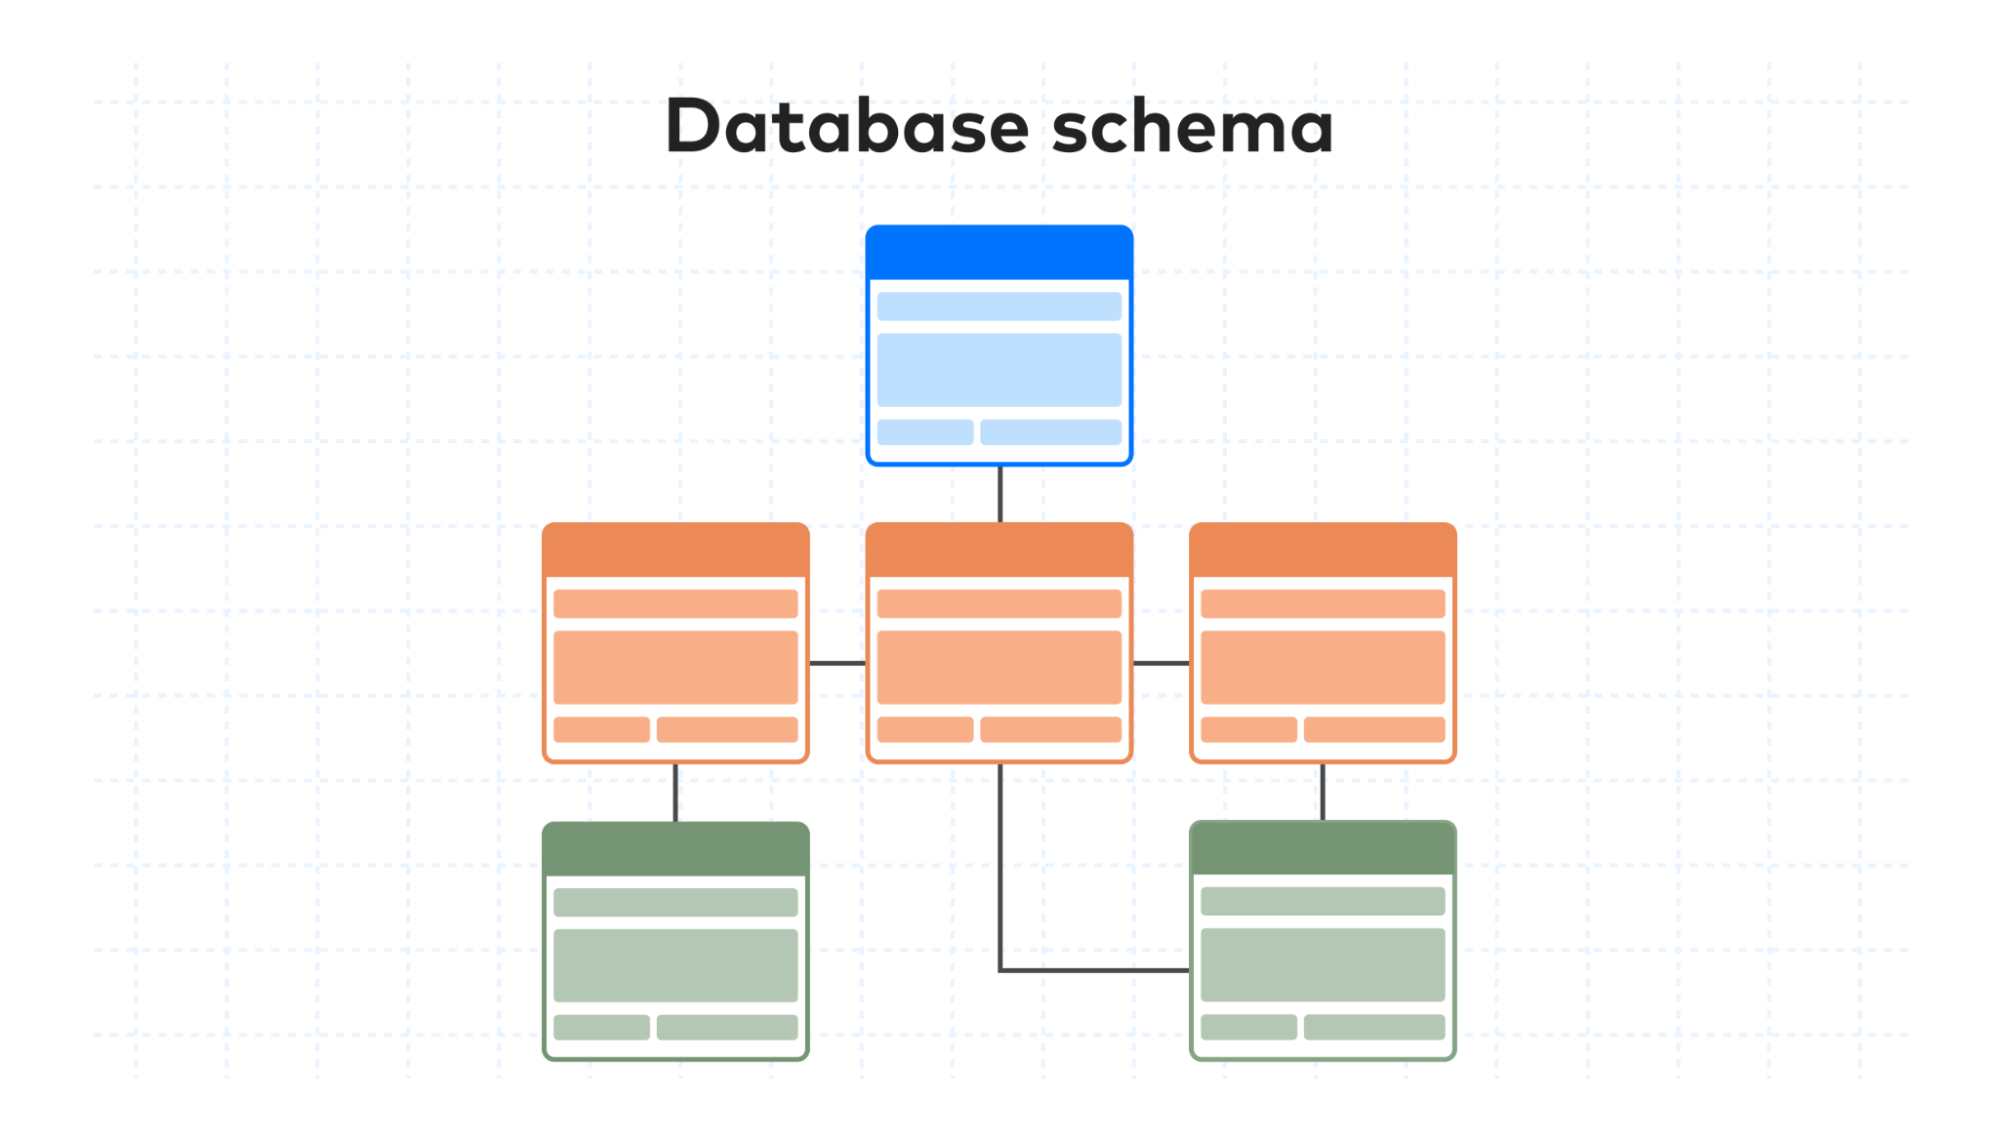
\includegraphics[width=0.9\textwidth]{img/database-schema.png}
    \end{figure}

\end{frame}


\begin{frame}{Schéma flexible}

    Donner example de schéma flexible

\end{frame}


\begin{frame}{Focus sur MongoDB}

\end{frame}

\begin{frame}{Étude de cas}

    Uber et MongoDB (gestion des trajets en temps réel).

    Problématique.
    Solution NoSQL choisie.
    Architecture mise en place.
    Résultats (performances, coûts).

\end{frame}

\begin{frame}[standout]

    Bases de données orientées colonne

\end{frame}

\begin{frame}{Caractéristiques des bases de données orientées colonne}

    \begin{definitionbox}
        Dans une base de données orientée colonne, les données sont stockées par \textbf{colonnes} plutôt que par lignes.

        Chaque ligne correspond à une clé unique, et les colonnes stockent des paires de \textbf{nom-colonne : valeur}, ce qui permet de regrouper des colonnes similaires pour une meilleure performance des requêtes en lecture.
    \end{definitionbox}

    \begin{noteblock}
        \begin{itemize}
            \item Optimisé pour les lectures massives sur des colonnes spécifiques.
            \item Très scalable et performant pour des requêtes analytiques.
        \end{itemize}
        $\hookrightarrow$ Idéal pour des applications nécessitant des analyses de grandes quantités de données.
    \end{noteblock}
\end{frame}

\begin{frame}{Bases de données orientées colonne}
    \begin{figure}[htb]
        \centering
        \begin{tikzpicture}
            \node[minimum width=3cm, minimum height=2cm] at (0, 0) {\includesvg[height=1.1cm]{img/db/cassandra.svg}};
            \node[minimum width=3cm, minimum height=2cm] at (4, 0) {\includesvg[height=0.9cm]{img/db/hbase.svg}};
            \node[minimum width=3cm, minimum height=2cm] at (0, -2) {\includesvg[height=0.7cm]{img/db/druid.svg}};
            \node[minimum width=3cm, minimum height=2cm] at (4, -2) {
\includegraphics[height=1.5cm]{img/db/scylla-db.png}};
            \node[minimum width=3cm, minimum height=2cm] at (0, -4) {
\includegraphics[height=1cm]{img/db/gcp-bigtable.png}};
            \node[minimum width=3cm, minimum height=2cm] at (4, -4) {
\includegraphics[height=1cm]{img/db/hypertable.png}};
        \end{tikzpicture}
    \end{figure}
\end{frame}

\begin{frame}{Exemple : distribution des données sur Cassandra}

    \begin{figure}
        \centering
        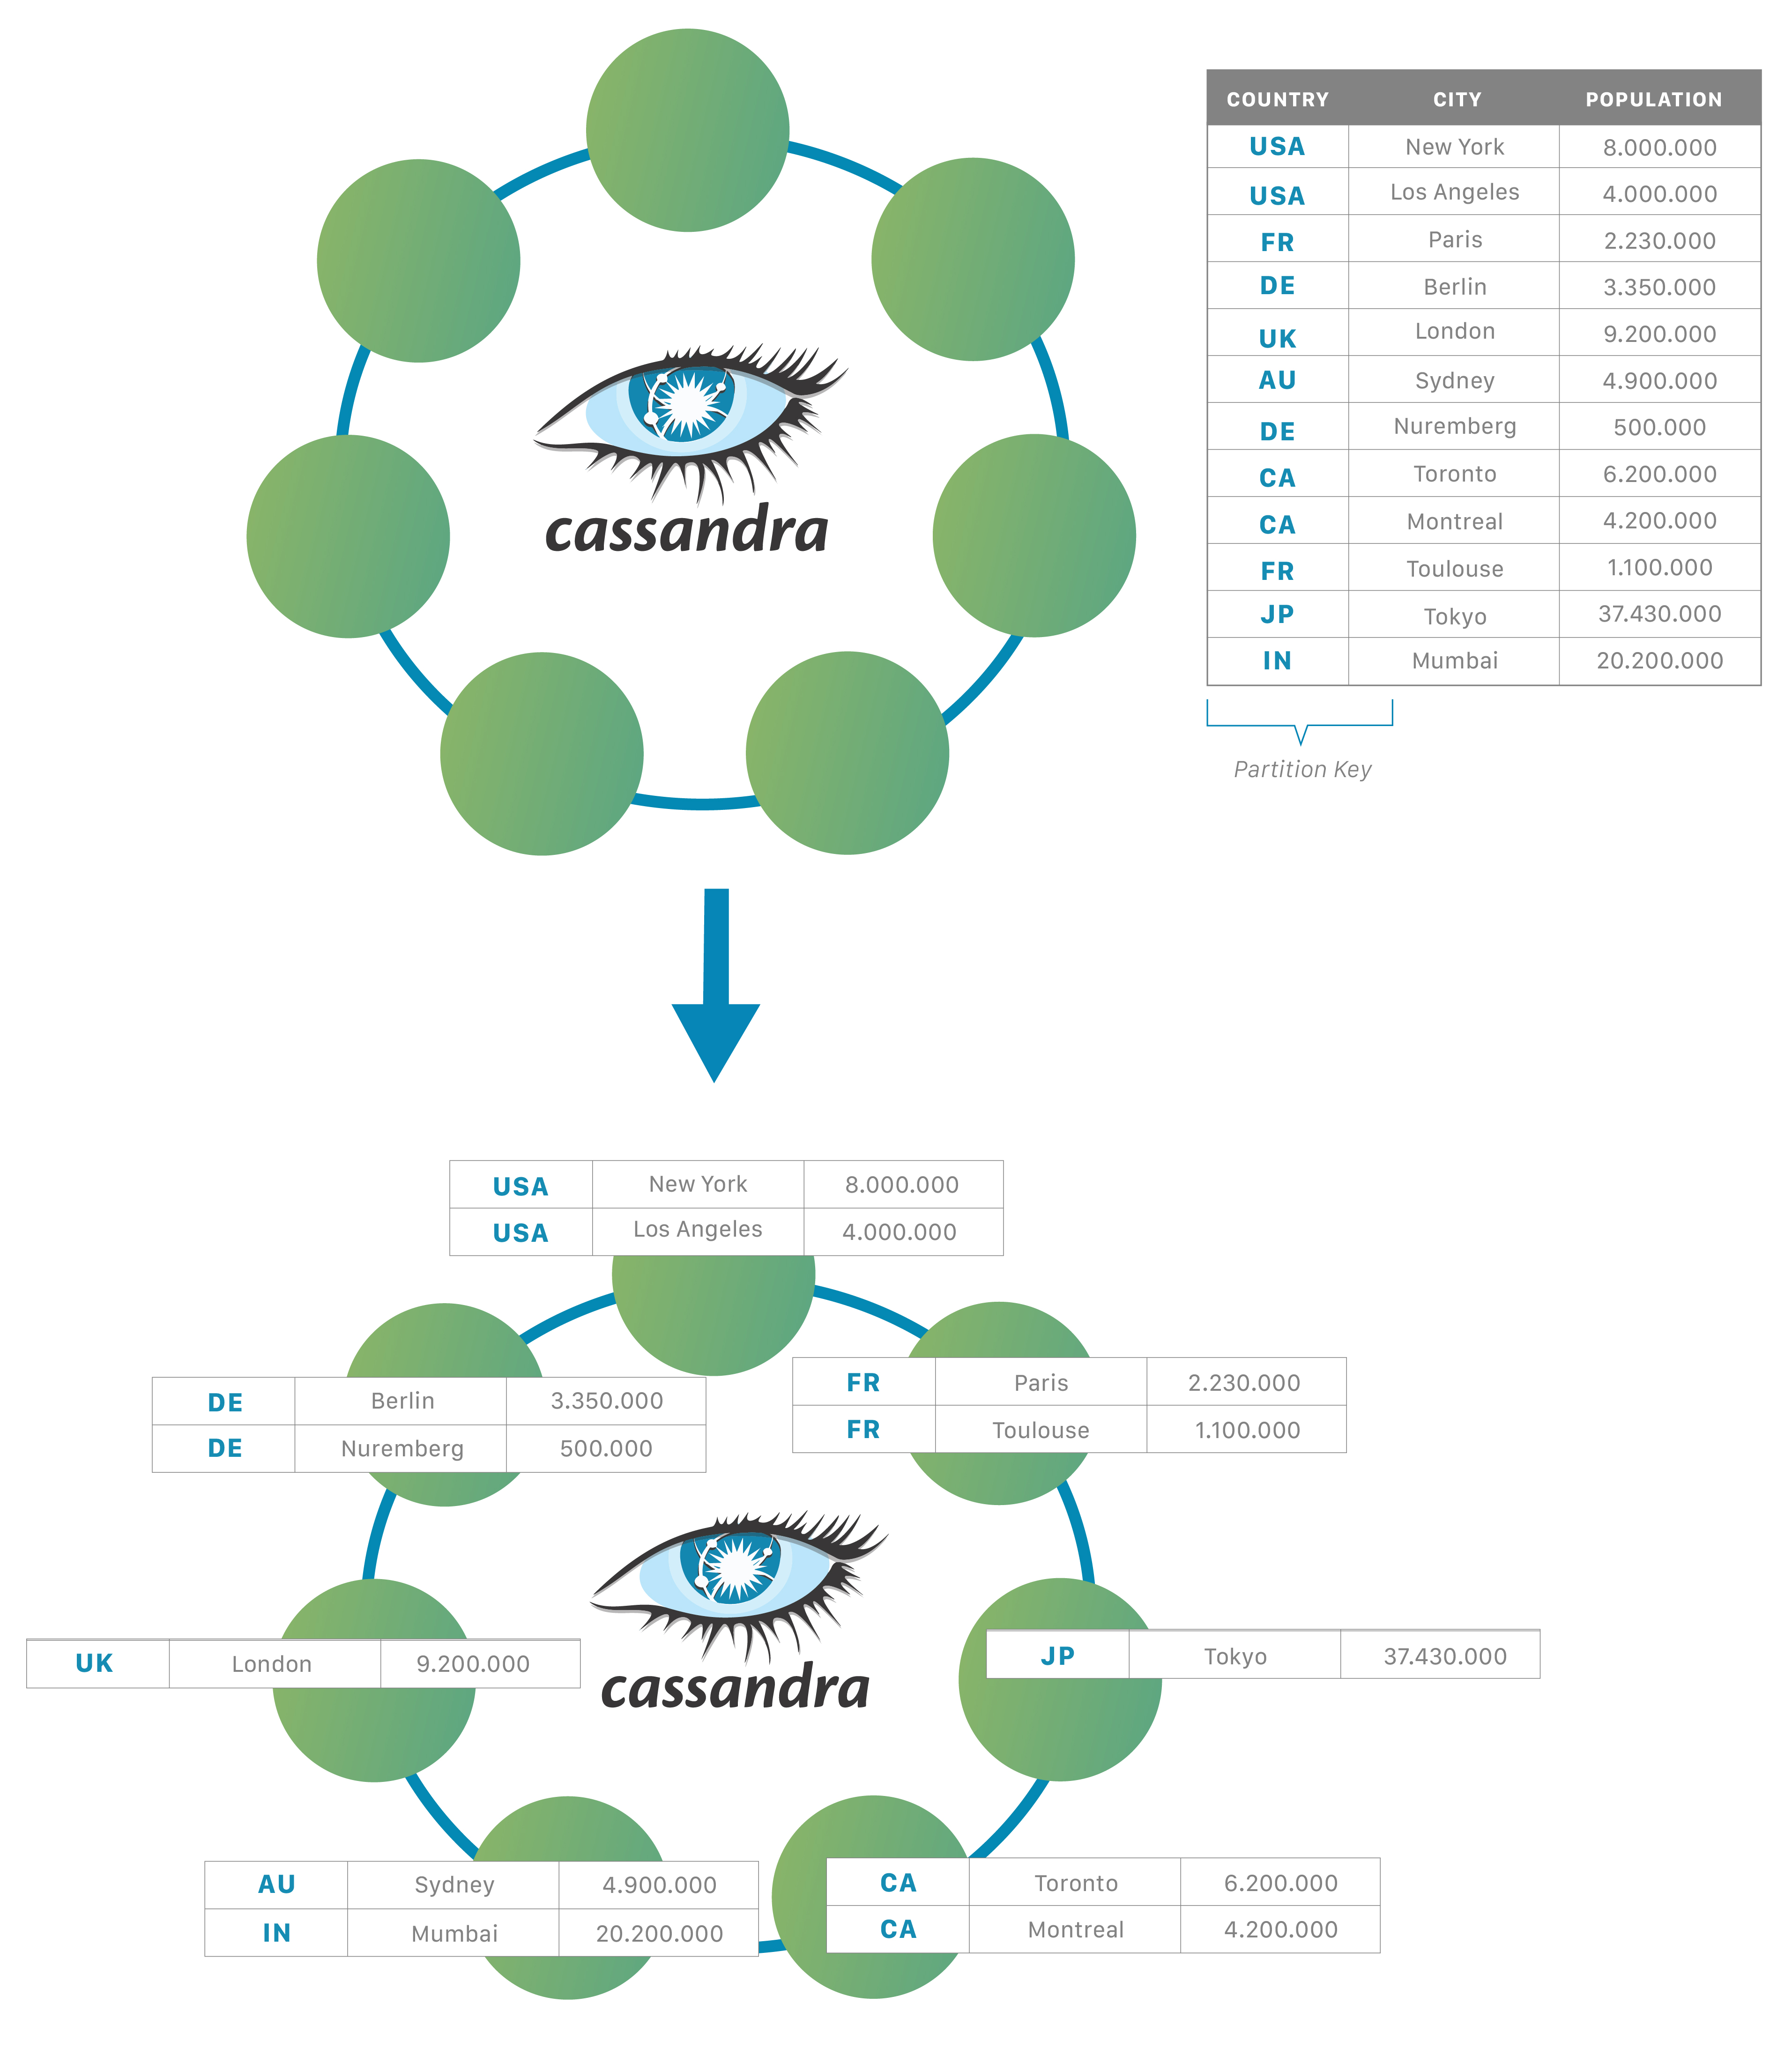
\includegraphics[width=0.8\textheight]{img/apache-cassandra-nodes.jpg}
    \end{figure}

\end{frame}

\begin{frame}{Cas d'usages des bases de données orientées colonne}

\begin{itemize}
    \item \textbf{Systèmes de gestion des données financières}\\
    $\hookrightarrow$ Permet d'extraire rapidement des colonnes spécifiques comme les prix ou les transactions sur de grands ensembles de données.
    \vspace{0.3cm}

    \item \textbf{Outils analytiques et de Big Data}\\
    $\hookrightarrow$ Optimisé pour les requêtes analytiques complexes sur des jeux de données massifs.
    \vspace{0.3cm}

    \item \textbf{Moteurs de recommandation}\\
    $\hookrightarrow$ Stocke des informations sur les utilisateurs et leurs préférences sous forme de colonnes, permettant une extraction rapide pour les recommandations en temps réel.
\end{itemize}
\end{frame}

\begin{frame}{Avantages et inconvénients des bases de données colonne}
\vfill
\prosbox{
    \textbf{Avantages}
    \begin{itemize}
        \item Très performant pour les requêtes en lecture sur des colonnes spécifiques.
        \item Scalabilité horizontale adaptée pour le traitement de données massives.
        \item Idéal pour des applications analytiques ou des systèmes OLAP.
    \end{itemize}
}
\vfill
\pause
\consbox{
    \textbf{Inconvénients}
    \begin{itemize}
        \item Moins efficace pour des écritures fréquentes ou des transactions complexes.
        \item Complexité accrue pour gérer les relations entre colonnes.
    \end{itemize}
}
\vfill
\end{frame}

\begin{frame}{Focus sur Apache Cassandra}

\end{frame}

\begin{frame}{Étude de cas}

    Netflix et Cassandra (scalabilité pour le streaming).

    Problématique.
    Solution NoSQL choisie.
    Architecture mise en place.
    Résultats (performances, coûts).

\end{frame}

\begin{frame}[standout]

    Bases de données orientées graphe

\end{frame}

\begin{frame}{Caractéristiques des bases de données graphe}

    \begin{definitionbox}
        Dans une base de données graphe, les données sont organisées en \textbf{nœuds}, \textbf{liens} et \textbf{propriétés} qui permettent de modéliser des relations complexes et dynamiques entre les entités. Les \textbf{nœuds} représentent les entités, les \textbf{liens} représentent les relations entre ces nœuds, et les \textbf{propriétés} fournissent des informations supplémentaires sur les nœuds et les liens.
    \end{definitionbox}

    \begin{noteblock}
        \begin{itemize}
            \item Représentation des relations complexes entre les données.
            \item Optimisé pour les requêtes de lecture et les opérations relationnelles.
        \end{itemize}
        % $\Longrightarrow$ Idéal pour des applications nécessitant des relations complexes et dynamiques entre les données.
        $\hookrightarrow$ Idéal pour des applications nécessitant des relations complexes et dynamiques entre les données.
    \end{noteblock}
\end{frame}

\begin{frame}{Bases de données graphe}
    \begin{figure}[htb]
        \centering
        \begin{tikzpicture}
            \node[minimum width=3cm, minimum height=2cm] at (0, 0) {\includesvg[height=1cm]{img/db/neo4j.svg}};
            \node[minimum width=3cm, minimum height=2cm] at (4, 0) {\includesvg[height=0.8cm]{img/db/arangodb.svg}};
            \node[minimum width=3cm, minimum height=2cm] at (0, -3) {
\includegraphics[height=1.3cm]{img/db/aws-neptune.png}};
            \node[minimum width=3cm, minimum height=2cm] at (4, -3) {\includesvg[height=1.3cm]{img/db/orientdb.svg}};
        \end{tikzpicture}
    \end{figure}
\end{frame}

\begin{frame}{Comment fonctionnent les bases de données graphe ?}

    \begin{figure}
        \centering
        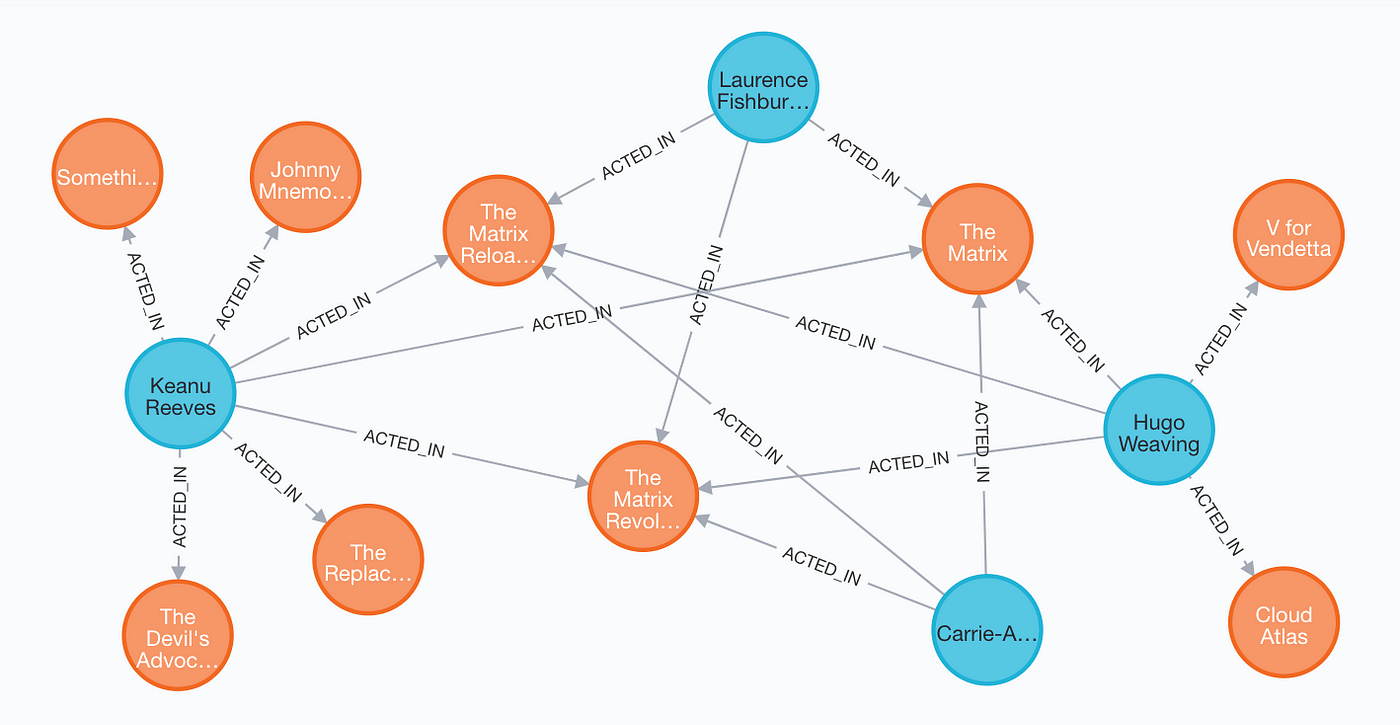
\includegraphics[width=0.8\textwidth]{img/neo4j-graph.png}
    \end{figure}

\end{frame}

\begin{frame}{Cas d'usages des bases de données graphe}

    \begin{itemize}
        \item \textbf{Réseaux sociaux}\\
        $\hookrightarrow$ Modélisation des relations entre utilisateurs, amis, groupes, et interactions pour des recommandations et des analyses sociales.
        \vspace{0.3cm}

        \item \textbf{Détection de fraude}\\
        $\hookrightarrow$ Analyse des connexions entre transactions et entités pour identifier des schémas de fraude ou des comportements suspects.
        \vspace{0.3cm}

        \item \textbf{Systèmes de recommandation}\\
        $\hookrightarrow$ Analyse des préférences des utilisateurs et des relations entre produits pour fournir des recommandations personnalisées.
        \vspace{0.3cm}

        \item \textbf{Gestion des réseaux de télécommunications}\\
        $\hookrightarrow$ Modélisation des réseaux de télécommunications et des relations entre équipements pour optimiser les performances et la maintenance.
    \end{itemize}
\end{frame}

\begin{frame}{Avantages et inconvénients des bases de données graphe}
    \vfill
    \prosbox{
        \textbf{Avantages}
        \begin{itemize}
            \item Excellente performance pour les requêtes impliquant des relations complexes.
            \item Flexibilité pour modéliser des structures de données dynamiques.
        \end{itemize}
    }
    \vfill
    \pause
    \consbox{
        \textbf{Inconvénients}
        \begin{itemize}
            \item Moins efficace pour les opérations non liées aux relations.
            \item Complexité accrue pour les utilisateurs non familiers avec la modélisation en graphe.
        \end{itemize}
    }
    \vfill
\end{frame}


\begin{frame}{Focus sur Neo4j}

\end{frame}

\begin{frame}{Étude de cas}

    LinkedIn et Neo4j (recommandations de connexions).

    Problématique.
    Solution NoSQL choisie.
    Architecture mise en place.
    Résultats (performances, coûts).

\end{frame}


% ------------------------------------------------------------------------------------------------------------------------------------------------------------------------

\begin{frame}{Retour sur le théorème CAP}

    Faire graphe et placer les différents systèmes (RDBMS, NoSQL, etc.)

\end{frame}

\begin{frame}{Retour sur le théorème CAP}

    \begin{figure}[htb]
        \resizebox{!}{0.85\textheight}{
        \begin{tikzpicture}
            % Circle 1: Consistency
            \draw[very thick, color=color-consistency, pattern=north east lines, pattern color=color-consistency] (0,0) circle (3cm);
            \node[fill=color-consistency, text=white, font=\bfseries, rounded corners] at (0,0.5) {Consistency};

            % Circle 2: Availability
            \draw[very thick, color=color-availability] (-2.1,-3.25) circle (3cm);
            \node[fill=color-availability, text=white, font=\bfseries, rounded corners] at (-2.75,-3.5) {Availability};

            % Circle 3: Partition Tolerance
            \draw[very thick, color=color-partition] (2.1,-3.25) circle (3cm);
            \node[fill=color-partition, text=white, font=\bfseries, rounded corners, align=left] at (2.75,-3.5) {Partition \\ tolerance};

            \node[fill=none, font=\bfseries, text=color-ca] (ca) at (-1.4,-1.5) {CA};
            \node[fill=none, font=\bfseries, text=color-cp] (cp) at (1.4,-1.5) {CP};
            \node[fill=none, font=\bfseries, text=color-ap] (ap) at (0,-3.7) {AP};

            % Unicorn
            \node[inner sep=0pt] (unicorn) at (0,-2.25) {
\includegraphics[width=1cm]{img/unicorn.png}};

            % Relationships
            % AP
            \node[yshift=-3.1cm] at (ap.south) {\includesvg[width=3cm]{img/db/cassandra.svg}};
            % CP
            \node[xshift=3.25cm, yshift=2.5cm] at (cp.east) {\includesvg[width=3cm]{img/db/mongodb.svg}};
            \node[xshift=4cm, yshift=1.2cm] at (cp.east) {\includesvg[width=3cm]{img/db/redis.svg}};
            % CA
            \node[xshift=-1.8cm, yshift=4.5cm] at (ca.west) {RDBMS};
            \node[xshift=-1.8cm, yshift=4.2cm] at (ca.west) {\includesvg[width=2cm]{img/db/postgresql.svg}};
            \node[xshift=-2.8cm, yshift=2.4cm] at (ca.west) {\includesvg[width=2cm]{img/db/mysql.svg}};
            \node[xshift=-3.5cm, yshift=1cm] at (ca.west) {\includesvg[width=2cm]{img/db/neo4j.svg}};
        \end{tikzpicture}
        }
    \end{figure}
\end{frame}

\begin{frame}{Performance}

    Faire un tableau comparatif des performances des différents types de bases de données NoSQL avec un exemple.

    Exemple : Quel est le revenu moyen des utilisateurs par pays ?

    SQLite (RDBMS) vs MongoDB (Document) vs Cassandra (Column) vs Neo4j (Graph)

\end{frame}

% Quiz

\begin{frame}[standout]

    Avez-vous été attentifs ?

    À vous de jouer !

\end{frame}

{
\setbeamercovered{transparent}

\begin{frame}{Q1}

    \textbf{Quels sont les quatre principaux types de bases de données NoSQL ?}

    \begin{itemize}
        \item \uncover<1>{\textcolor{kh-red}{Colonne, Clé-Valeur, XML, Graph}}
        \item \uncover<1>{\textcolor{kh-blue}{JSON, Colonne, Document, Graph}}
        \item \uncover<1>{\textcolor{kh-green}{Clé-Valeur, Table, Document, SQL}}
        \item \textbf<2>{\textcolor{kh-yellow}{Clé-Valeur, Colonne, Document, Graph}}
    \end{itemize}

\end{frame}

\begin{frame}{Q2}

    \textbf{Dans une base de données de type document, sous quelle forme les données sont-elles stockées ?}

    \begin{itemize}
        \item \uncover<1>{\textcolor{kh-red}{Clé-valeur}}
        \item \textbf<2>{\textcolor{kh-blue}{JSON ou BSON}}
        \item \uncover<1>{\textcolor{kh-green}{Table}}
        \item \uncover<1>{\textcolor{kh-yellow}{Colonne}}
    \end{itemize}

\end{frame}

\begin{frame}{Q3}

    \textbf{Quelle base de données NoSQL est conçue pour les requêtes de graphe complexe ?}

    \begin{itemize}
        \item \uncover<1>{\textcolor{kh-red}{Redis}}
        \item \uncover<1>{\textcolor{kh-blue}{Apache Cassandra}}
        \item \textbf<2>{\textcolor{kh-green}{Neo4j}}
        \item \uncover<1>{\textcolor{kh-yellow}{MongoDB}}
    \end{itemize}

\end{frame}

\begin{frame}{Q4}

    \textbf{Quelle base de données est plus adaptée pour un jeu vidéo ?}

    En tant que membre d'une équipe de développeurs de jeux, vous avez été chargé de concevoir un moyen de suivre les possessions des joueurs (achetées dans un catalogue, échangées entre joueurs ou via des récompenses). Les possessions sont classées en vêtements, outils, livres et pièces de monnaie. Les joueurs peuvent avoir un nombre illimité de possessions de n'importe quel type. Les joueurs peuvent rechercher d'autres joueurs possédant des types de possessions particuliers pour des échanges. Le concepteur du jeu informe qu'il y aura probablement de nouveaux types de possessions et de nouvelles façons de les acquérir à l'avenir. Quel type de base de données recommanderiez-vous d'utiliser ?

    \begin{itemize}
        \item \uncover<1>{\textcolor{kh-red}{Base de données transactionnelle}}
        \item \uncover<1>{\textcolor{kh-blue}{Base de données orientée colonne}}
        \item \textbf<2>{\textcolor{kh-green}{Base de données orientée document}}
        \item \uncover<1>{\textcolor{kh-yellow}{Base de données analytique}}
    \end{itemize}

\end{frame}

\begin{frame}{Q5}

    \textbf{Quelle base de données est plus adaptée pour un logiciel ?}

    Un développeur de logiciels vous demande conseil sur le stockage des données. Il dispose de centaines de milliers d'objets JSON de 1 Ko qui doivent être accessibles en moins d'une milliseconde si possible. Tous les objets sont référencés par une clé. Il n'est pas nécessaire de rechercher des valeurs dans le contenu de la structure JSON. Quel type de base de données NoSQL recommanderiez-vous ?

    \begin{itemize}
        \item \uncover<1>{\textcolor{kh-red}{Base de données orientée graphe}}
        \item \uncover<1>{\textcolor{kh-blue}{Base de données analytique}}
        \item \uncover<1>{\textcolor{kh-green}{Base de données orientée colonne}}
        \item \textbf<2>{\textcolor{kh-yellow}{Base de données clé-valeur}}
    \end{itemize}

\end{frame}

\begin{frame}{Q6}

    \textbf{Quelle base de données est plus adaptée pour un logiciel ?}

    Une développeuse de logiciels vous demande conseil sur le stockage de données. Il a des centaines de milliers d'objets JSON de 10 Ko qui doivent pouvoir être recherchés par la plupart des attributs de la structure JSON. Quel type de base de données NoSQL recommanderiez-vous ?

    \begin{itemize}
        \item \textbf<2>{\textcolor{kh-red}{Base de données orientée document}}
        \item \uncover<1>{\textcolor{kh-blue}{Base de données orientée colonne}}
        \item \uncover<1>{\textcolor{kh-green}{Base de données analytique}}
        \item \uncover<1>{\textcolor{kh-yellow}{Base de données clé-valeur}}
    \end{itemize}

\end{frame}

%\begin{frame}{Q7}
%
%    \textbf{Une programmeuse conçoit une base de données pour prendre en charge les requêtes ad hoc. Quel type de schéma de données est-il susceptible d'utiliser ?}
%
%    \textit{Une requête ad hoc est une requête qui est créée pour répondre à un besoin d'information spécifique, souvent de manière ponctuelle, et qui n'est pas prévue ou récurrente dans les opérations normales de la base de données.}
%
%    \begin{itemize}
%        \item \uncover<1>{\textcolor{kh-red}{Online Transaction Processing (OLTP)}}
%        \item \textbf<2>{\textcolor{kh-blue}{Online Analytical Processing (OLAP)}}
%        \item \uncover<1>{\textcolor{kh-green}{Schéma normalisé}}
%        \item \uncover<1>{\textcolor{kh-yellow}{Schéma Dénormalisé}}
%        \item \uncover<1>{\textcolor{kh-teal}{Graphe de connaissances}}
%    \end{itemize}
%
%\end{frame}

%\begin{frame}{Q8}
%
%    \textbf{}
%
%    \begin{itemize}
%        \item \uncover<1>{\textcolor{kh-red}{}}
%        \item \uncover<1>{\textcolor{kh-blue}{}}
%        \item \textbf<2>{\textcolor{kh-green}{}}
%        \item \uncover<1>{\textcolor{kh-yellow}{}}
%    \end{itemize}
%
%\end{frame}
%
%\begin{frame}{Q9}
%
%    \textbf{}
%
%    \begin{itemize}
%        \item \uncover<1>{\textcolor{kh-red}{}}
%        \item \uncover<1>{\textcolor{kh-blue}{}}
%        \item \textbf<2>{\textcolor{kh-green}{}}
%        \item \uncover<1>{\textcolor{kh-yellow}{}}
%    \end{itemize}
%
%\end{frame}
%
%\begin{frame}{Q10}
%
%    \textbf{}
%
%    \begin{itemize}
%        \item \uncover<1>{\textcolor{kh-red}{}}
%        \item \uncover<1>{\textcolor{kh-blue}{}}
%        \item \textbf<2>{\textcolor{kh-green}{}}
%        \item \uncover<1>{\textcolor{kh-yellow}{}}
%    \end{itemize}
%
%\end{frame}

}


\begin{frame}{Pour la prochaine séance}

    \textbf{(1) NoSQL} : réaliser les TP de prérequis

    \begin{itemize}
        \item Introduction à git
        \item Utilisation d'un terminal
        \item Conteneurisation avec Docker
    \end{itemize}

    \vspace{1cm}

    \textbf{(2) SAÉ migration de données vers ou depuis un environnement NoSQL}

    Pour la prochaine séance, constituer des binômes pour la SAÉ (un trinôme si groupe impair).

\end{frame}


\end{document}
